% Capitolul 4: Selecția modelului și managementul riscului
% Statistica Piețelor Financiare
% Program de licență, Academia de Studii Economice din București

\documentclass[9pt, aspectratio=169, t]{beamer}

% Asigură încadrarea conținutului pe diapozitive
\setbeamersize{text margin left=8mm, text margin right=8mm}

%=============================================================================
% CONFIGURARE TEMĂ ȘI STIL
%=============================================================================
\usetheme{default}
% Utilizăm tema implicită pentru control curat al antetului/subsolului

% Paletă de Culori (potrivită cu PDF-ul Redispatch)
\definecolor{MainBlue}{RGB}{26, 58, 110}
\definecolor{AccentBlue}{RGB}{26, 58, 110}
\definecolor{IDAred}{RGB}{205, 0, 0}
\definecolor{DarkGray}{RGB}{51, 51, 51}
\definecolor{MediumGray}{RGB}{128, 128, 128}
\definecolor{LightGray}{RGB}{248, 248, 248}
\definecolor{VeryLightGray}{RGB}{235, 235, 235}
\definecolor{KeynoteGray}{RGB}{218, 218, 218}
\definecolor{SectionGray}{RGB}{120, 120, 120}
\definecolor{FooterGray}{RGB}{100, 100, 100}
\definecolor{Crimson}{RGB}{220, 53, 69}
\definecolor{Forest}{RGB}{46, 125, 50}
\definecolor{Amber}{RGB}{181, 133, 63}
\definecolor{Orange}{RGB}{230, 126, 34}
\definecolor{Purple}{RGB}{142, 68, 173}

% Fundal gradient (gradient Keynote exact 315°: alb la RGB 218,218,218)
\setbeamertemplate{background}{%
    \begin{tikzpicture}[remember picture, overlay]
        \shade[shading=axis, shading angle=315,
        top color=white, bottom color=KeynoteGray]
        (current page.south west) rectangle (current page.north east);
    \end{tikzpicture}%
}
% Culoare solidă de rezervă pentru compatibilitate
\setbeamercolor{background canvas}{bg=}

\setbeamercolor{palette primary}{bg=MainBlue, fg=white}
\setbeamercolor{palette secondary}{bg=MainBlue!85, fg=white}
\setbeamercolor{palette tertiary}{bg=MainBlue!70, fg=white}
\setbeamercolor{structure}{fg=MainBlue}
\setbeamercolor{title}{fg=IDAred}
\setbeamercolor{frametitle}{fg=IDAred, bg=}
\setbeamercolor{block title}{bg=MainBlue, fg=white}
\setbeamercolor{block body}{bg=VeryLightGray, fg=DarkGray}
\setbeamercolor{block title alerted}{bg=Crimson, fg=white}
\setbeamercolor{block body alerted}{bg=Crimson!8, fg=DarkGray}
\setbeamercolor{block title example}{bg=Forest, fg=white}
\setbeamercolor{block body example}{bg=Forest!8, fg=DarkGray}
\setbeamercolor{item}{fg=MainBlue}

% Culori subsol (suprascriu albastrul temei Madrid)
\setbeamercolor{author in head/foot}{fg=FooterGray, bg=}
\setbeamercolor{title in head/foot}{fg=FooterGray, bg=}
\setbeamercolor{date in head/foot}{fg=FooterGray, bg=}
\setbeamercolor{section in head/foot}{fg=FooterGray, bg=}
\setbeamercolor{subsection in head/foot}{fg=FooterGray, bg=}

% Stiluri marcatori (se aplică peste tot inclusiv în blocuri)
\setbeamertemplate{itemize item}{\color{MainBlue}$\boxdot$}
\setbeamertemplate{itemize subitem}{\color{MainBlue}$\blacktriangleright$}
\setbeamertemplate{itemize subsubitem}{\color{MainBlue}\tiny$\bullet$}
\setbeamertemplate{itemize/enumerate body begin}{\normalsize}
\setbeamertemplate{itemize/enumerate subbody begin}{\normalsize}

% Item spacing - compact style
\setlength{\leftmargini}{10pt}       % Level 1: minimal indent
\setlength{\leftmarginii}{10pt}      % Level 2: minimal additional indent
% Compact list spacing (zero extra space before/after lists in blocks)
\makeatletter
\def\@listi{\leftmargin\leftmargini \topsep 0pt \parsep 0pt \itemsep 0pt}
\def\@listii{\leftmargin\leftmarginii \topsep 0pt \parsep 0pt \itemsep 0pt}
\makeatother

\setbeamertemplate{navigation symbols}{}

%=============================================================================
% ANTET PERSONALIZAT
%=============================================================================
\setbeamertemplate{headline}{%
    \vskip10pt%
    \hbox to \paperwidth{%
        \hskip0.5cm%
        {\small\color{FooterGray}\thesection.\ \renewcommand{\hyperlink}[2]{##2}\insertsectionhead}%
        \hfill%
        \showlevel\hspace{4pt}%
        \textcolor{FooterGray}{\small\insertframenumber}%
        \hskip0.5cm%
    }%
    \vskip4pt%
    {\color{\currentlevelcolor}\hrule height 1.5pt}%
    \global\slidelevelnum=0%
    \gdef\currentlevelcolor{FooterGray}%
}

%=============================================================================
% SUBSOL PERSONALIZAT
%=============================================================================
\usepackage{fontawesome5}

\setbeamertemplate{footline}{%
    {\color{FooterGray}\hrule height 0.4pt}%
    \vskip4pt%
    \hbox to \paperwidth{%
        \hskip0.5cm%
        \textcolor{FooterGray}{\small Statistica Piețelor Financiare}%
        \hfill%
        \raisebox{-0.1em}{%
            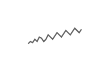
\begin{tikzpicture}[x=0.08em, y=0.08em, line width=0.4pt]
                \draw[FooterGray] (0,3) -- (1,4) -- (2,3.5) -- (3,5) -- (4,4) -- (5,6) -- (6,5.5) -- (7,4) -- (8,5) -- (9,7) -- (10,6) -- (11,5) -- (12,6.5) -- (13,8) -- (14,7) -- (15,6) -- (16,7.5) -- (17,9) -- (18,8) -- (19,7) -- (20,8.5) -- (21,10) -- (22,9) -- (23,8) -- (24,9.5);
            \end{tikzpicture}%
        }%
        \hskip0.5cm%
    }%
    \vskip6pt%
}

%=============================================================================
% PACHETE
%=============================================================================
\usepackage[utf8]{inputenc}
\usepackage[T1]{fontenc}
\usepackage{amsmath, amssymb, amsthm}
\usepackage{mathtools}
\usepackage{bm}
\usepackage{tikz}
\usetikzlibrary{arrows.meta, positioning, shapes, calc, decorations.pathreplacing, shadings}
\usepackage{booktabs}
\usepackage{multirow}
\usepackage{array}
\usepackage{graphicx}
\usepackage{hyperref}
\usepackage{colortbl}
\usepackage{pifont}
\hypersetup{colorlinks=true, linkcolor=MainBlue, urlcolor=MainBlue}
\graphicspath{{../../logos/}{../../charts/}{../../photos/}}
\hfuzz=2pt  % Suppress tiny overfull warnings (<2pt)
\vfuzz=2pt  % Suppress tiny vertical overfull warnings (<2pt)

%=============================================================================
% COMANDA QUANTLET
%=============================================================================
\newcommand{\quantlet}[2]{%
    \vspace{-0.25cm}%
    \hfill\href{#2}{%
        \raisebox{-0.15em}{
\includegraphics[height=0.7em]{ql_logo.png}}%
        \textcolor{MainBlue}{\tiny\ #1}%
    }\par%
}

%=============================================================================
% PAGINĂ TITLU PERSONALIZATĂ
%=============================================================================
\defbeamertemplate*{title page}{hybrid}[1][]
{
    \vspace{0.2cm}
    % Rând logo-uri - antet superior (cu linkuri clickabile)
    \begin{center}
        \href{https://www.ase.ro}{
\includegraphics[height=1.0cm]{ase_logo.png}}\hspace{0.3cm}%
        \href{https://theida.net}{
\includegraphics[height=1.0cm]{ida_logo.png}}\hspace{0.3cm}%
        \href{https://blockchain-research-center.com}{
\includegraphics[height=1.0cm]{brc_logo.png}}\hspace{0.3cm}%
        \href{https://www.ai4efin.ase.ro}{
\includegraphics[height=1.0cm]{ai4efin_logo.png}}\hspace{0.3cm}%
        \href{https://ipe.ro/new}{
\includegraphics[height=1.0cm]{acad_logo.png}}\hspace{0.3cm}%
        \href{https://www.digital-finance-msca.com}{
\includegraphics[height=1.0cm]{msca_logo.png}}%
    \end{center}

    \vspace{0.6cm}

    % Titlu principal cu logo-uri Q pe părți (cu linkuri clickabile)
    \begin{center}
        \begin{minipage}{0.1\textwidth}
            \centering
            \href{https://quantlet.com}{
\includegraphics[height=1.1cm]{ql_logo.png}}
        \end{minipage}%
        \begin{minipage}{0.78\textwidth}
            \centering
            {\LARGE\bfseries\usebeamercolor[fg]{title}\inserttitle}

            \vspace{0.3cm}

            {\usebeamerfont{subtitle}\usebeamercolor[fg]{title}\insertsubtitle}
        \end{minipage}%
        \begin{minipage}{0.1\textwidth}
            \centering
            \href{https://quantinar.com}{
\includegraphics[height=1.1cm]{qr_logo.png}}
        \end{minipage}
    \end{center}

    \vspace{0.6cm}

    % Autori (aliniere la stânga)
    \hspace{0.5cm}\begin{minipage}[t]{0.9\textwidth}
        \usebeamerfont{author}\insertauthor
    \end{minipage}

    \vspace{0.3cm}

    % Institut/Afilieri (aliniere la stânga)
    \hspace{0.5cm}\begin{minipage}[t]{0.9\textwidth}
        \raggedright\small\insertinstitute
    \end{minipage}
}

%=============================================================================
% MEDII PENTRU TEOREME
%=============================================================================
\theoremstyle{definition}
\setbeamertemplate{theorems}[numbered]
\newtheorem{defn}{Definiție}
\newtheorem{thm}{Teoremă}
\newtheorem{prop}{Propoziție}
\newtheorem{rmk}{Observație}

%=============================================================================
% CENTRED MINIPAGE
%=============================================================================
\newenvironment{cminipage}[1]{%
    \par\noindent\hfill\begin{minipage}{#1}\ignorespaces
}{%
    \end{minipage}\hfill\null\par
}

%=============================================================================
% COMENZI PERSONALIZATE
%=============================================================================
\newcommand{\E}{\mathbb{E}}
\newcommand{\Var}{\text{Var}}
\newcommand{\Cov}{\text{Cov}}
\newcommand{\Corr}{\text{Corr}}
\newcommand{\R}{\mathbb{R}}
\newcommand{\N}{\mathbb{N}}
\newcommand{\Z}{\mathbb{Z}}
\newcommand{\B}{\mathbf{B}}
\newcommand{\imark}{\textcolor{MainBlue}{\textbullet}}
\newcommand{\RMSE}{\text{RMSE}}
\newcommand{\MAE}{\text{MAE}}
\newcommand{\MAPE}{\text{MAPE}}

% Indicatoare nivel academic pe slide-uri  (numeric \ifnum — bulletproof in beamer templates)
\newcount\slidelevelnum
\global\slidelevelnum=0
\makeatletter
\newcommand{\slidelevel}[1]{%
    \global\slidelevelnum=0%
    \def\tmp@SL{#1}\def\tmp@SLy{Y3}\def\tmp@SLm{MSc}\def\tmp@SLp{PhD}%
    \ifx\tmp@SL\tmp@SLy \global\slidelevelnum=1\fi%
    \ifx\tmp@SL\tmp@SLm \global\slidelevelnum=2\fi%
    \ifx\tmp@SL\tmp@SLp \global\slidelevelnum=3\fi%
}
\makeatother
\gdef\currentlevelcolor{FooterGray}
\newcommand{\showlevel}{%
    \ifnum\slidelevelnum=1%
        \colorbox{Forest}{\strut\textcolor{white}{\sffamily\bfseries\fontsize{8}{9}\selectfont Y3}}%
        \gdef\currentlevelcolor{Forest}%
    \fi%
    \ifnum\slidelevelnum=2%
        \colorbox{MainBlue}{\strut\textcolor{white}{\sffamily\bfseries\fontsize{8}{9}\selectfont MSc}}%
        \gdef\currentlevelcolor{MainBlue}%
    \fi%
    \ifnum\slidelevelnum=3%
        \colorbox{Crimson}{\strut\textcolor{white}{\sffamily\bfseries\fontsize{8}{9}\selectfont PhD}}%
        \gdef\currentlevelcolor{Crimson}%
    \fi%
    \ifnum\slidelevelnum=0%
        \gdef\currentlevelcolor{FooterGray}%
    \fi%
}


%=============================================================================
% INFORMATII TITLU
%=============================================================================
\title[Statistica Piețelor Financiare]{Statistica Piețelor Financiare}
\subtitle{Capitolul 4: Selecția modelului și managementul riscului}
\author[D.T. Pele, A. Amza]{\texorpdfstring{\begin{tabular}[t]{@{}l@{}}Daniel Traian PELE \\ Antoaneta Amza\end{tabular}}{Daniel Traian PELE, Antoaneta Amza}}
\institute{Academia de Studii Economice din București\\
IDA Institute Digital Assets\\
Blockchain Research Center\\
AI4EFin Artificial Intelligence for Energy Finance\\
Academia Română, Institutul de Prognoză Economică\\
MSCA Digital Finance}
\date{}

\begin{document}

% Pagina de titlu (fara antet/subsol)
{
\setbeamertemplate{headline}{}
\setbeamertemplate{footline}{}
\begin{frame}
    \titlepage
\end{frame}
}

%=============================================================================
% OBIECTIVE DE INVATARE
%=============================================================================
\begin{frame}{Obiective de învățare}
    \begin{block}{La sfârșitul acestui curs, veți fi capabili să:}
    \begin{enumerate}
        \item[\textcolor{MainBlue}{\textbf{1.}}] \textbf{Comparați} distribuțiile folosind criterii AIC, BIC, QQ și teste formale
        \item[\textcolor{MainBlue}{\textbf{2.}}] \textbf{Explicați} rolul copulelor în modelarea dependenței de coadă (\textit{tail dependence})
        \item[\textcolor{MainBlue}{\textbf{3.}}] \textbf{Calculați} VaR și Expected Shortfall sub diferite ipoteze distribuționale
        \item[\textcolor{MainBlue}{\textbf{4.}}] \textbf{Efectuați} backtesting VaR (Kupiec, Christoffersen)
        \item[\textcolor{MainBlue}{\textbf{5.}}] \textbf{Evaluați} modele GARCH cu inovații non-Gaussiene
    \end{enumerate}
    \end{block}
\end{frame}

%=============================================================================
% CUPRINS
%=============================================================================
{
\setbeamertemplate{headline}{%
    \vskip10pt%
    \hbox to \paperwidth{\hskip0.5cm\hfill\hskip0.5cm}%
    \vskip4pt%
    {\color{FooterGray}\hrule height 0.4pt}%
}
\begin{frame}{}
    {\color{FooterGray}\hrule height 0.4pt}
    \vspace{0.1cm}
    {\Large\textcolor{IDAred}{\textbf{Cuprins}}}
    \vspace{0.2cm}
    {\small
    \begin{itemize}
        \item Compararea distribuțiilor și selecția modelului
        \item Copule și dependența de coadă (\textit{tail dependence})
        \item Implicații pentru managementul riscului
        \item Extensii moderne
        \item Rezumat
    \end{itemize}
    }
\end{frame}
}

\section{Compararea distribuțiilor și selecția modelului}

%--- Y3 Slide 1 ---
\slidelevel{Y3}
\begin{frame}{Comparație vizuală a distribuțiilor}
\begin{center}
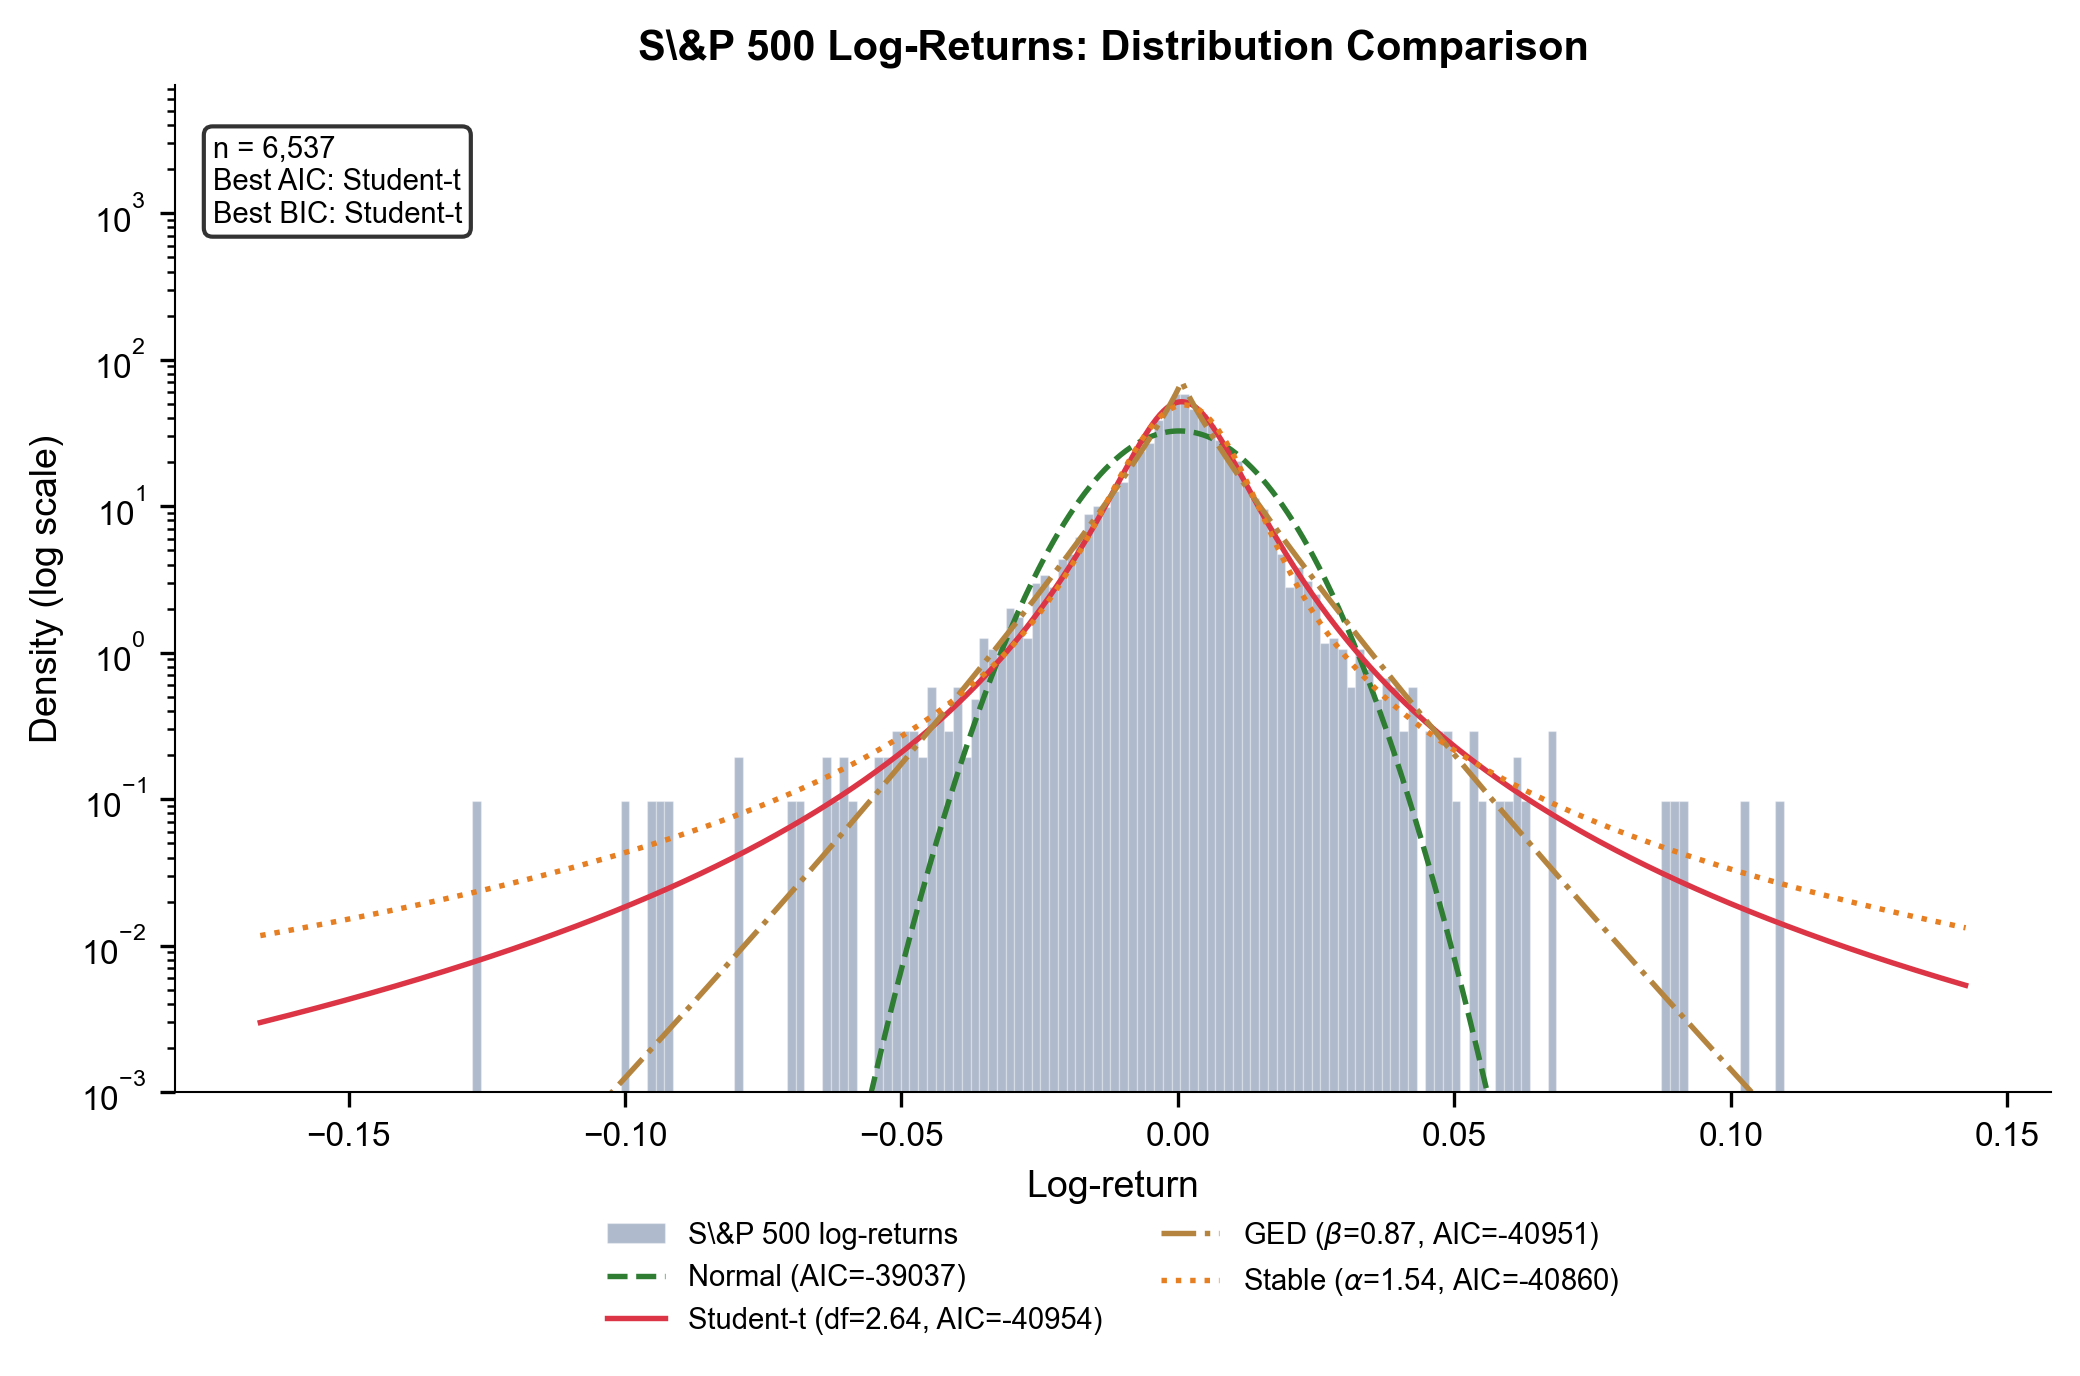
\includegraphics[width=0.5\textwidth]{ch2_dist_comparison_overlay.png}
\end{center}
\quantlet{SFM\_ch2\_dist\_comparison}{https://github.com/QuantLet/Stat_fin_markets/tree/master/Ch_02/SFM_ch2_distribution_comparison}
\begin{itemize}
\item Histogramă cu suprapuneri ajustate: Normală, Student-$t$, Stabilă
\item Care distribuție surprinde cel mai bine centrul, umerii și cozile?
\end{itemize}
\end{frame}

%--- Y3 Slide 2 ---
\slidelevel{Y3}
\begin{frame}{Grafice QQ}
\begin{columns}[T]
\begin{column}{0.48\textwidth}
\begin{center}
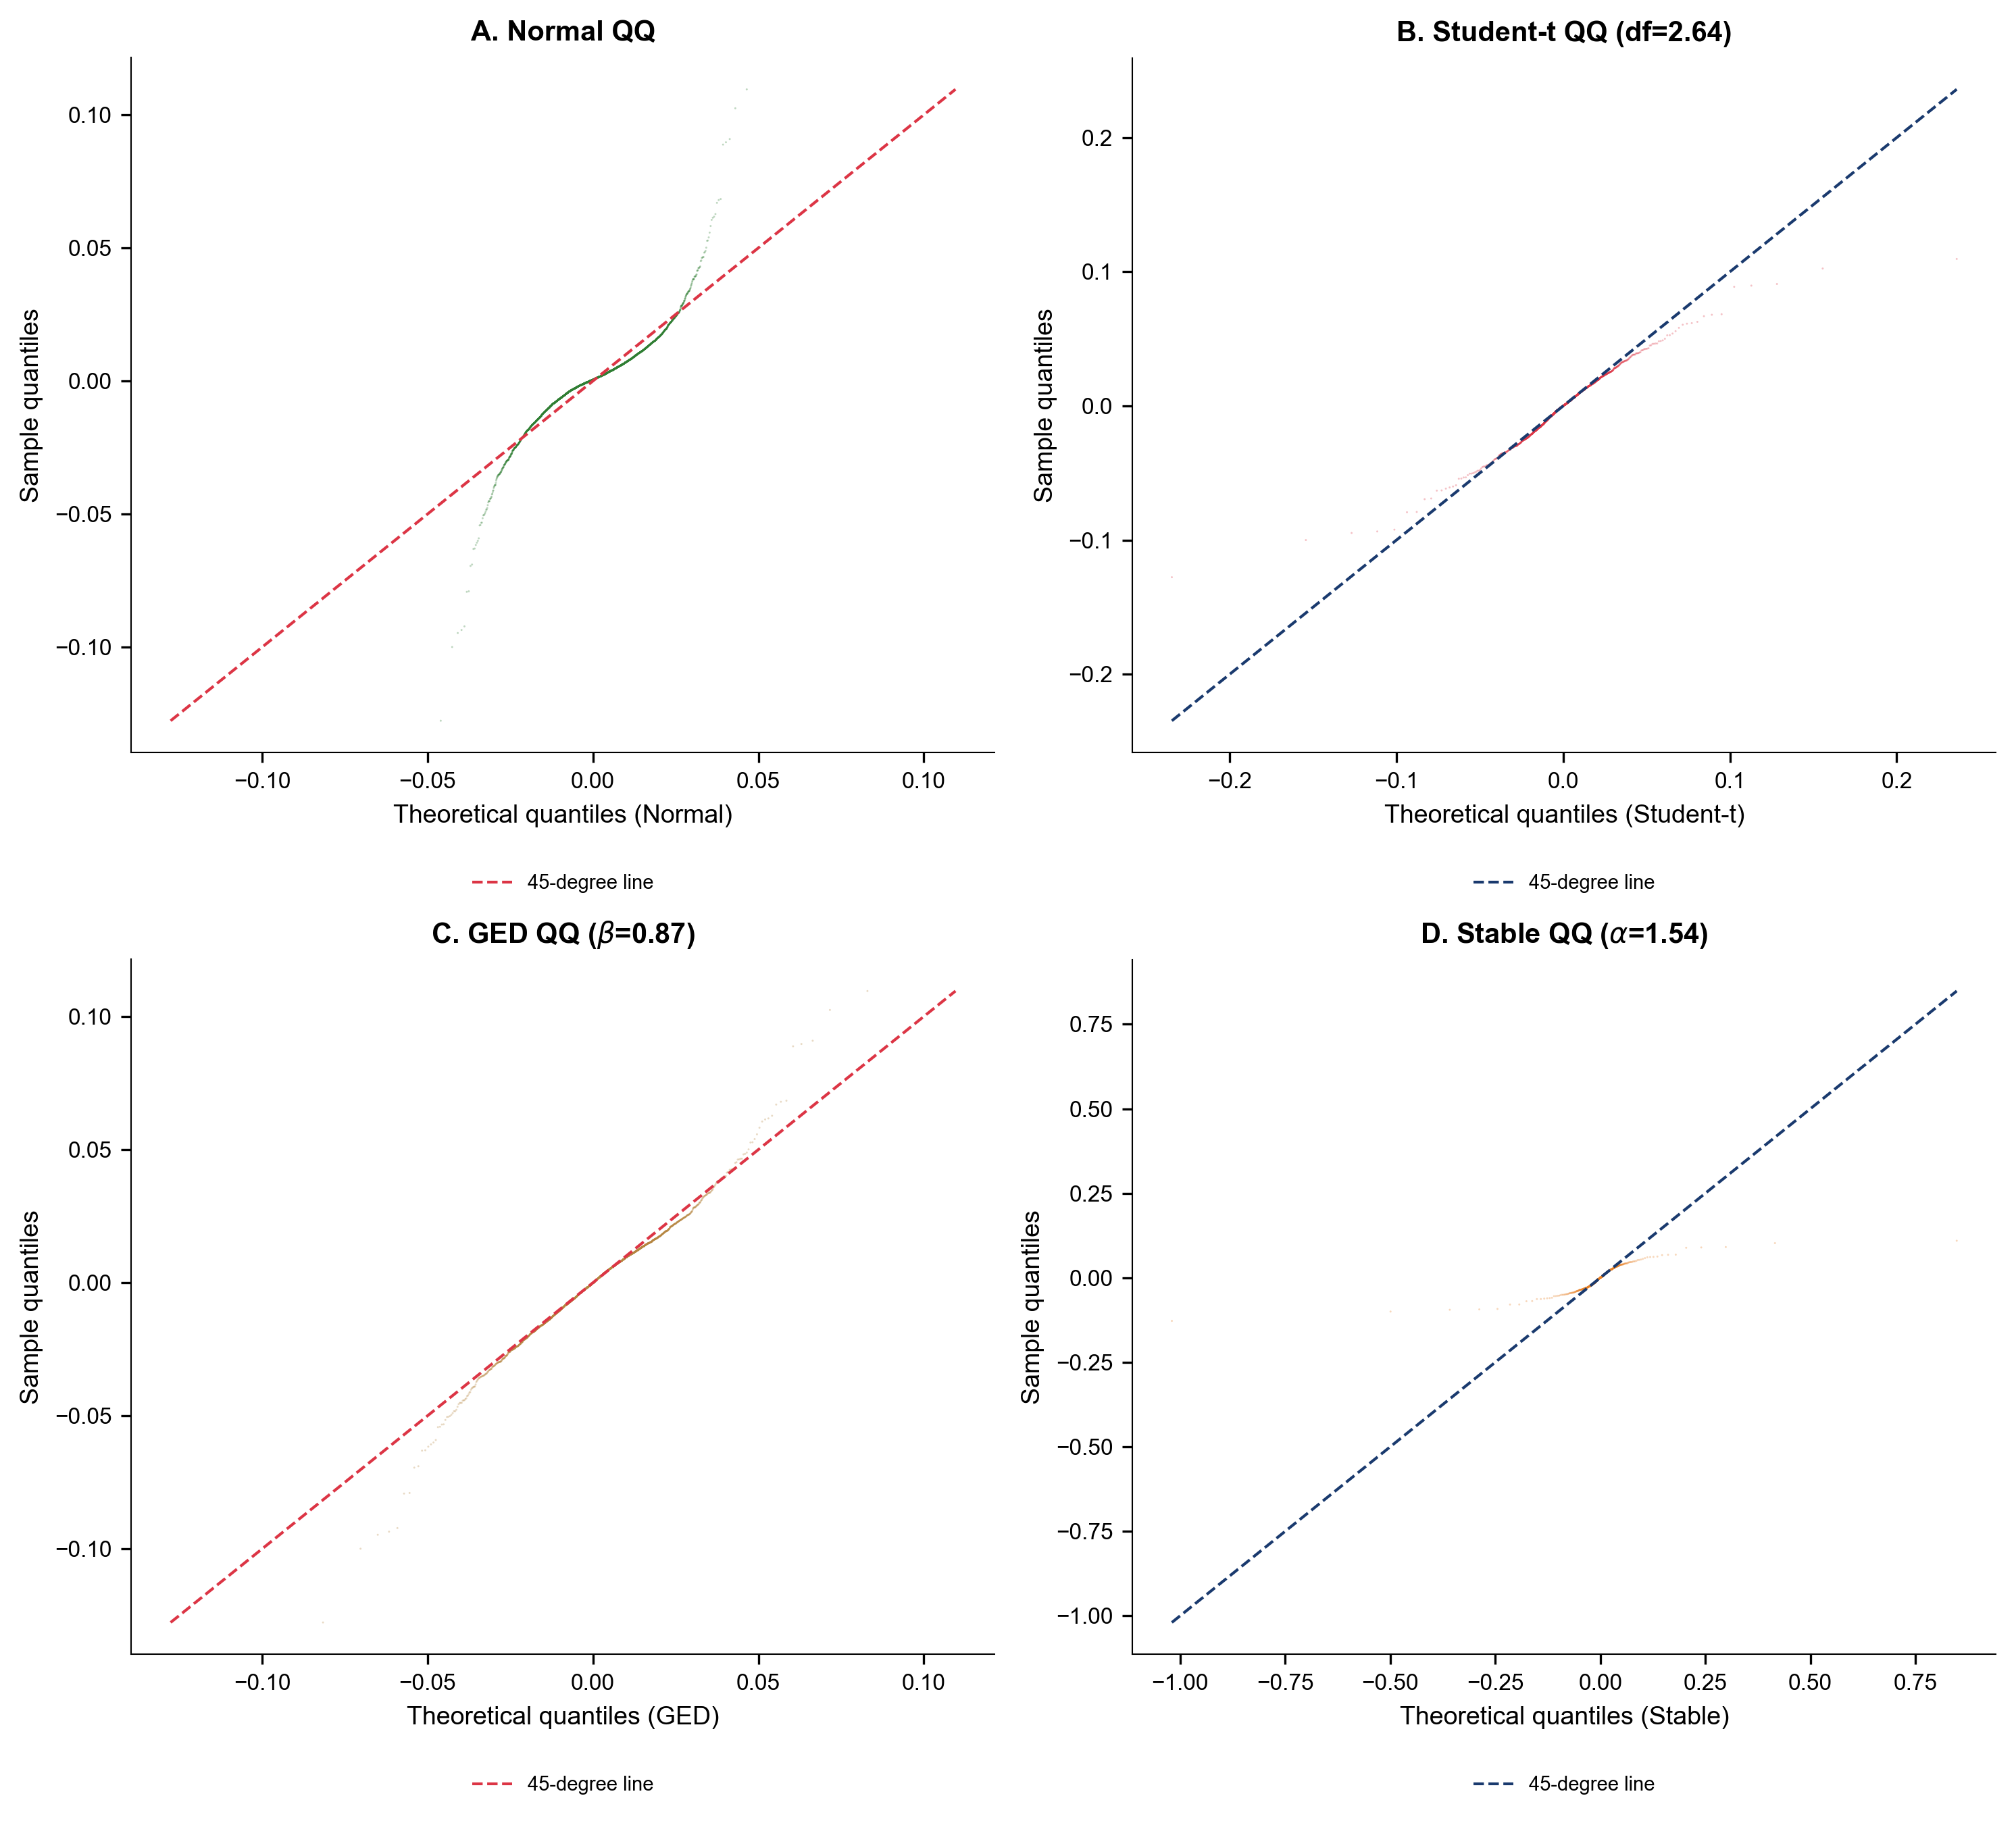
\includegraphics[width=0.85\textwidth]{ch2_dist_comparison_qq.png}
\end{center}
\quantlet{SFM\_ch2\_qq}{https://github.com/QuantLet/Stat_fin_markets/tree/master/Ch_02/SFM_ch2_distribution_comparison}
\end{column}
\begin{column}{0.48\textwidth}
\begin{itemize}
\item \textbf{Grafic QQ}: cuantile date vs.\ distribuție teoretică
\item Ajustare perfectă $\Rightarrow$ pe linia de 45$^\circ$; \textbf{formă de S}: cozi mai groase
\item QQ sub distribuția normală: abateri sistematice; Student-$t$: mai aproape de 45$^\circ$
\end{itemize}
\end{column}
\end{columns}
\end{frame}

%--- Y3 Slide 2b ---
\slidelevel{Y3}
\begin{frame}{Checklist: Fapt stilizat $\to$ Distribuție}
\begin{center}
\renewcommand{\arraystretch}{1.2}
\footnotesize
\begin{tabular}{l c c c c c}
\toprule
\textbf{Fapt stilizat} & \textbf{Normal} & \textbf{Student-$t$} & \textbf{Skew-$t$} & \textbf{Stabilă} & \textbf{EVT} \\
\midrule
Cozi groase & \textcolor{Crimson}{\ding{55}} & \textcolor{Forest}{\checkmark} & \textcolor{Forest}{\checkmark} & \textcolor{Forest}{\checkmark} & \textcolor{Forest}{\checkmark} \\
Asimetrie & \textcolor{Crimson}{\ding{55}} & \textcolor{Crimson}{\ding{55}} & \textcolor{Forest}{\checkmark} & \textcolor{Forest}{\checkmark} & \textcolor{Crimson}{\ding{55}} \\
Clusterizare vol. & \textcolor{Crimson}{\ding{55}} & \textcolor{Crimson}{\ding{55}} & \textcolor{Crimson}{\ding{55}} & \textcolor{Crimson}{\ding{55}} & \textcolor{Crimson}{\ding{55}} \\
Kurtosis $> 3$ & \textcolor{Crimson}{\ding{55}} & \textcolor{Forest}{\checkmark} & \textcolor{Forest}{\checkmark} & \textcolor{Forest}{\checkmark} & --- \\
Varianță infinită & \textcolor{Crimson}{\ding{55}} & $\ast$ & \textcolor{Crimson}{\ding{55}} & \textcolor{Forest}{\checkmark} & --- \\
\bottomrule
\end{tabular}
\end{center}

\begin{itemize}
\item $\ast$ Student-$t$: varianță infinită (\textit{infinite variance}) doar dacă $\nu \leq 2$ (rar în practică)
\item \textbf{Nicio distribuție statică} nu captează clusterizarea volatilității (\textit{volatility clustering}) $\Rightarrow$ necesită modele dinamice (GARCH)
\item Tabelul ghidează selecția: dacă datele prezintă asimetrie, eliminăm distribuția normală și Student-$t$ simetrică
\end{itemize}
\end{frame}

%--- Y3 Slide 3 ---
\slidelevel{Y3}
\begin{frame}{Graficul log-log al cozilor}
\begin{center}
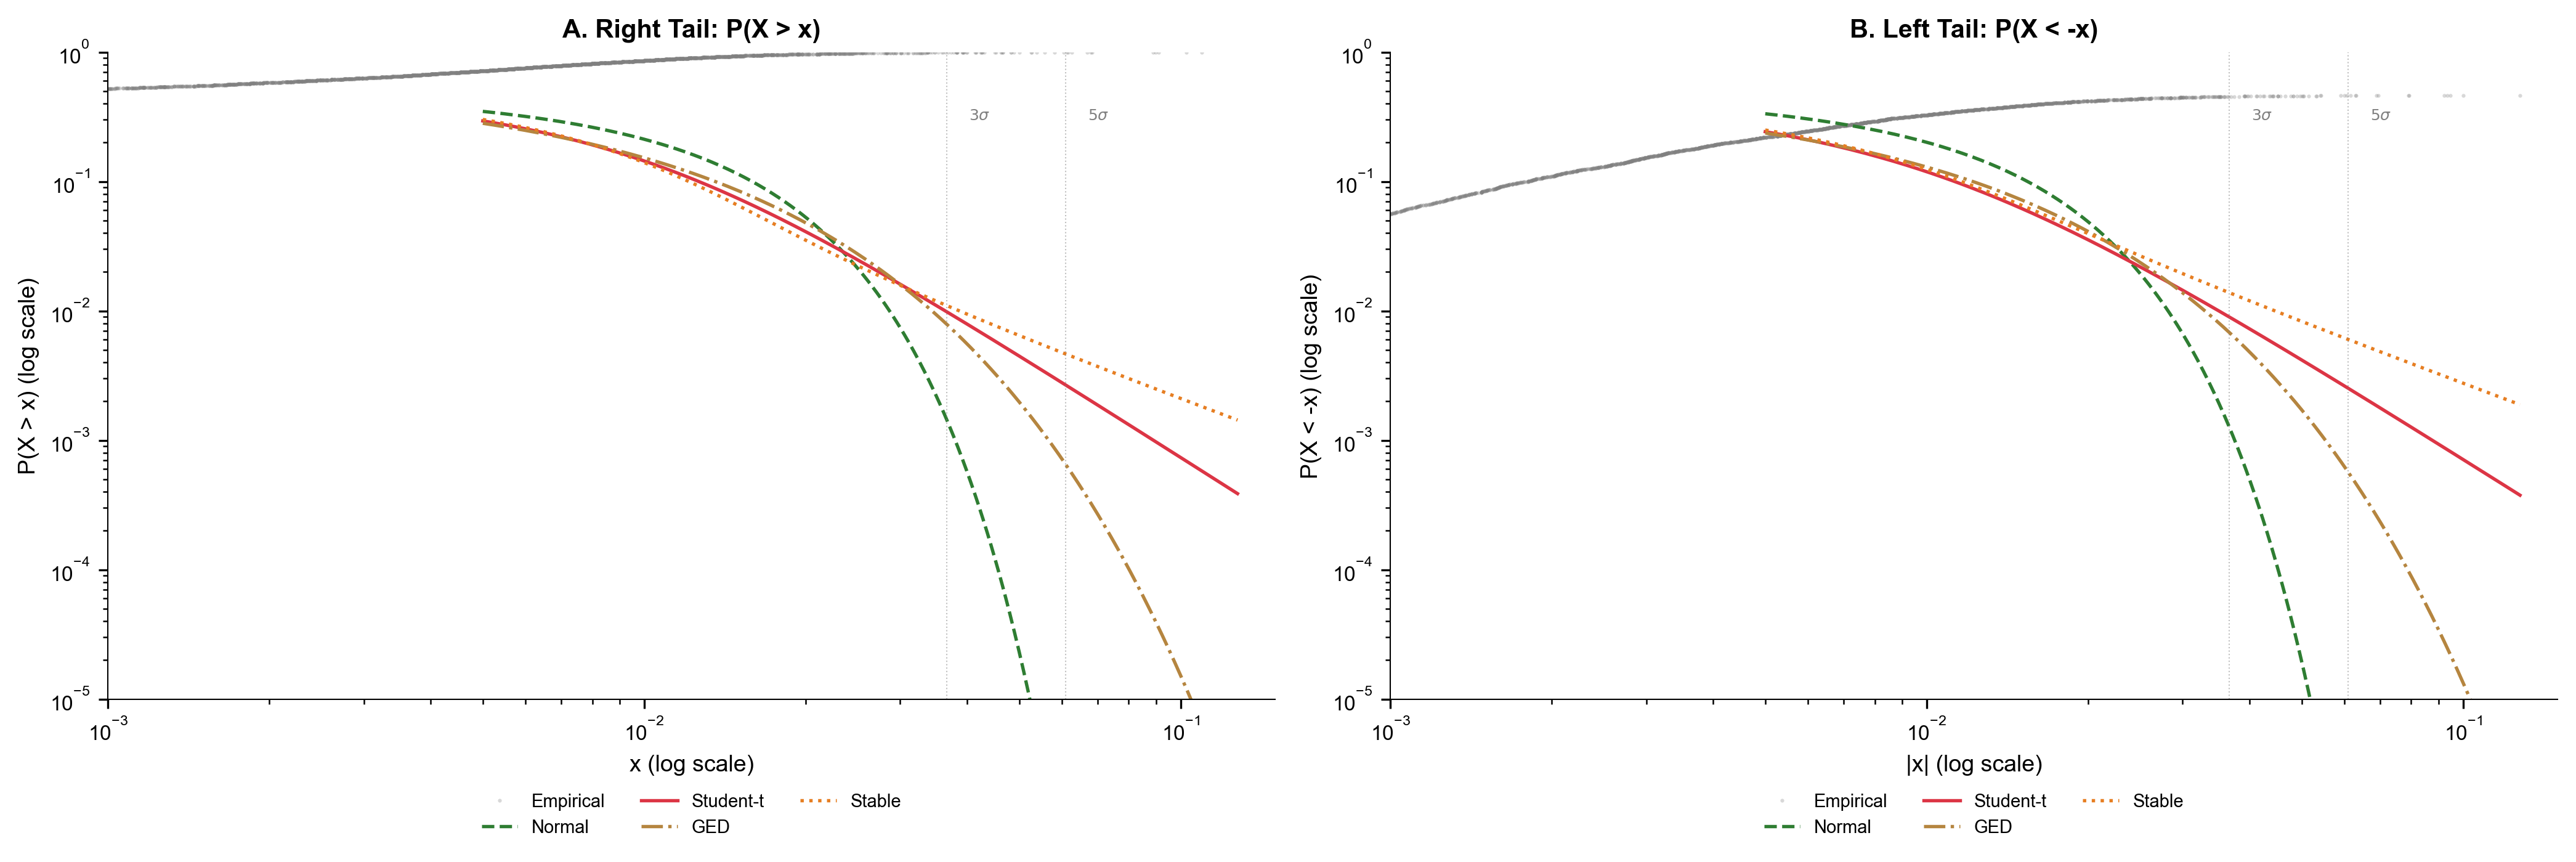
\includegraphics[width=0.65\textwidth]{ch2_dist_comparison_tails.png}
\end{center}
\quantlet{SFM\_ch2\_log\_tails}{https://github.com/QuantLet/Stat_fin_markets/tree/master/Ch_02/SFM_ch2_distribution_comparison}
\begin{itemize}
\item Reprezentăm $\ln P(|X| > x)$ vs.\ $\ln x$
\item Coadă tip lege putere (\textit{power law}): dreaptă cu panta $-\alpha$
\item Normală: se curbează în jos (descreștere exponențială)
\item Student-$t$ și Stabilă: aproximativ liniare (descreștere tip lege putere)
\end{itemize}
\end{frame}

%--- MSc Slide 4 ---
\slidelevel{MSc}
\begin{frame}{Criterii informaționale}
\begin{block}{Formulele AIC și BIC}
\[
\text{AIC} = -2\ell(\hat{\theta}) + 2k, \qquad \text{BIC} = -2\ell(\hat{\theta}) + k\ln n
\]
\vspace{-0.2cm}
{\small $\ell(\hat{\theta})$ = log-verosimilitatea maximizată;\; $k$ = nr.\ parametri;\; $n$ = dimensiune eșantion}
\end{block}
\vspace{0.2cm}
\begin{center}
\renewcommand{\arraystretch}{1.5}
\large
\begin{tabular}{lccc}
\toprule
\textbf{Distribuție} & \textbf{$k$} & \textbf{AIC} & \textbf{BIC} \\
\midrule
Normală & 2 & Cel mai mare & Cel mai mare \\
Student-$t$ & 3 & Mai mic & Mai mic \\
Student-$t$ asim. & 4 & \textcolor{Forest}{\textbf{Cel mai mic}} & \textcolor{Forest}{\textbf{Cel mai mic}} \\
Stabilă & 4 & Comparabil & Comparabil \\
\bottomrule
\end{tabular}
\end{center}
\end{frame}

%--- MSc Slide 4b ---
\slidelevel{MSc}
\begin{frame}{Teste formale de adecvare și raportul de verosimilitate}
\begin{block}{Teste de adecvare (GoF)}
\begin{itemize}\setlength{\itemsep}{2pt}
\item \textbf{KS}: $H_0\!: F = F_\theta$ vs.\ $H_1\!: F \neq F_\theta$;\quad $D_n = \sup_x |F_n(x) - F_\theta(x)|$
\item \textbf{AD}: aceeași ipoteză, dar ponderat pe cozi:\\ $A^2 = -n - \frac{1}{n}\sum (2i\!-\!1)\bigl[\ln F_\theta(x_{(i)}) + \ln(1\!-\!F_\theta(x_{(n+1-i)}))\bigr]$
\end{itemize}
\end{block}
\vspace{0.15cm}
\begin{block}{Test raport de verosimilitate (LR) --- modele imbricate}
$H_0$: modelul restrâns (ex.\ Normală) \quad vs.\ $H_1$: modelul general (ex.\ Student-$t$)
\[
\boxed{\;LR = -2\bigl[\ell(\hat{\theta}_0) - \ell(\hat{\theta}_1)\bigr] \;\sim\; \chi^2(k_1 - k_0)\;}
\]
{\small Respingem $H_0$ dacă $LR > \chi^2_{k_1-k_0;\,1-\alpha}$. Ex.: Normal ($k_0\!=\!2$) vs.\ $t$ ($k_1\!=\!3$): $\chi^2(1)$.}
\end{block}
\end{frame}

%--- MSc Slide 5 ---
\slidelevel{MSc}
\begin{frame}{Comparație cuprinzătoare a modelelor}
\begin{center}
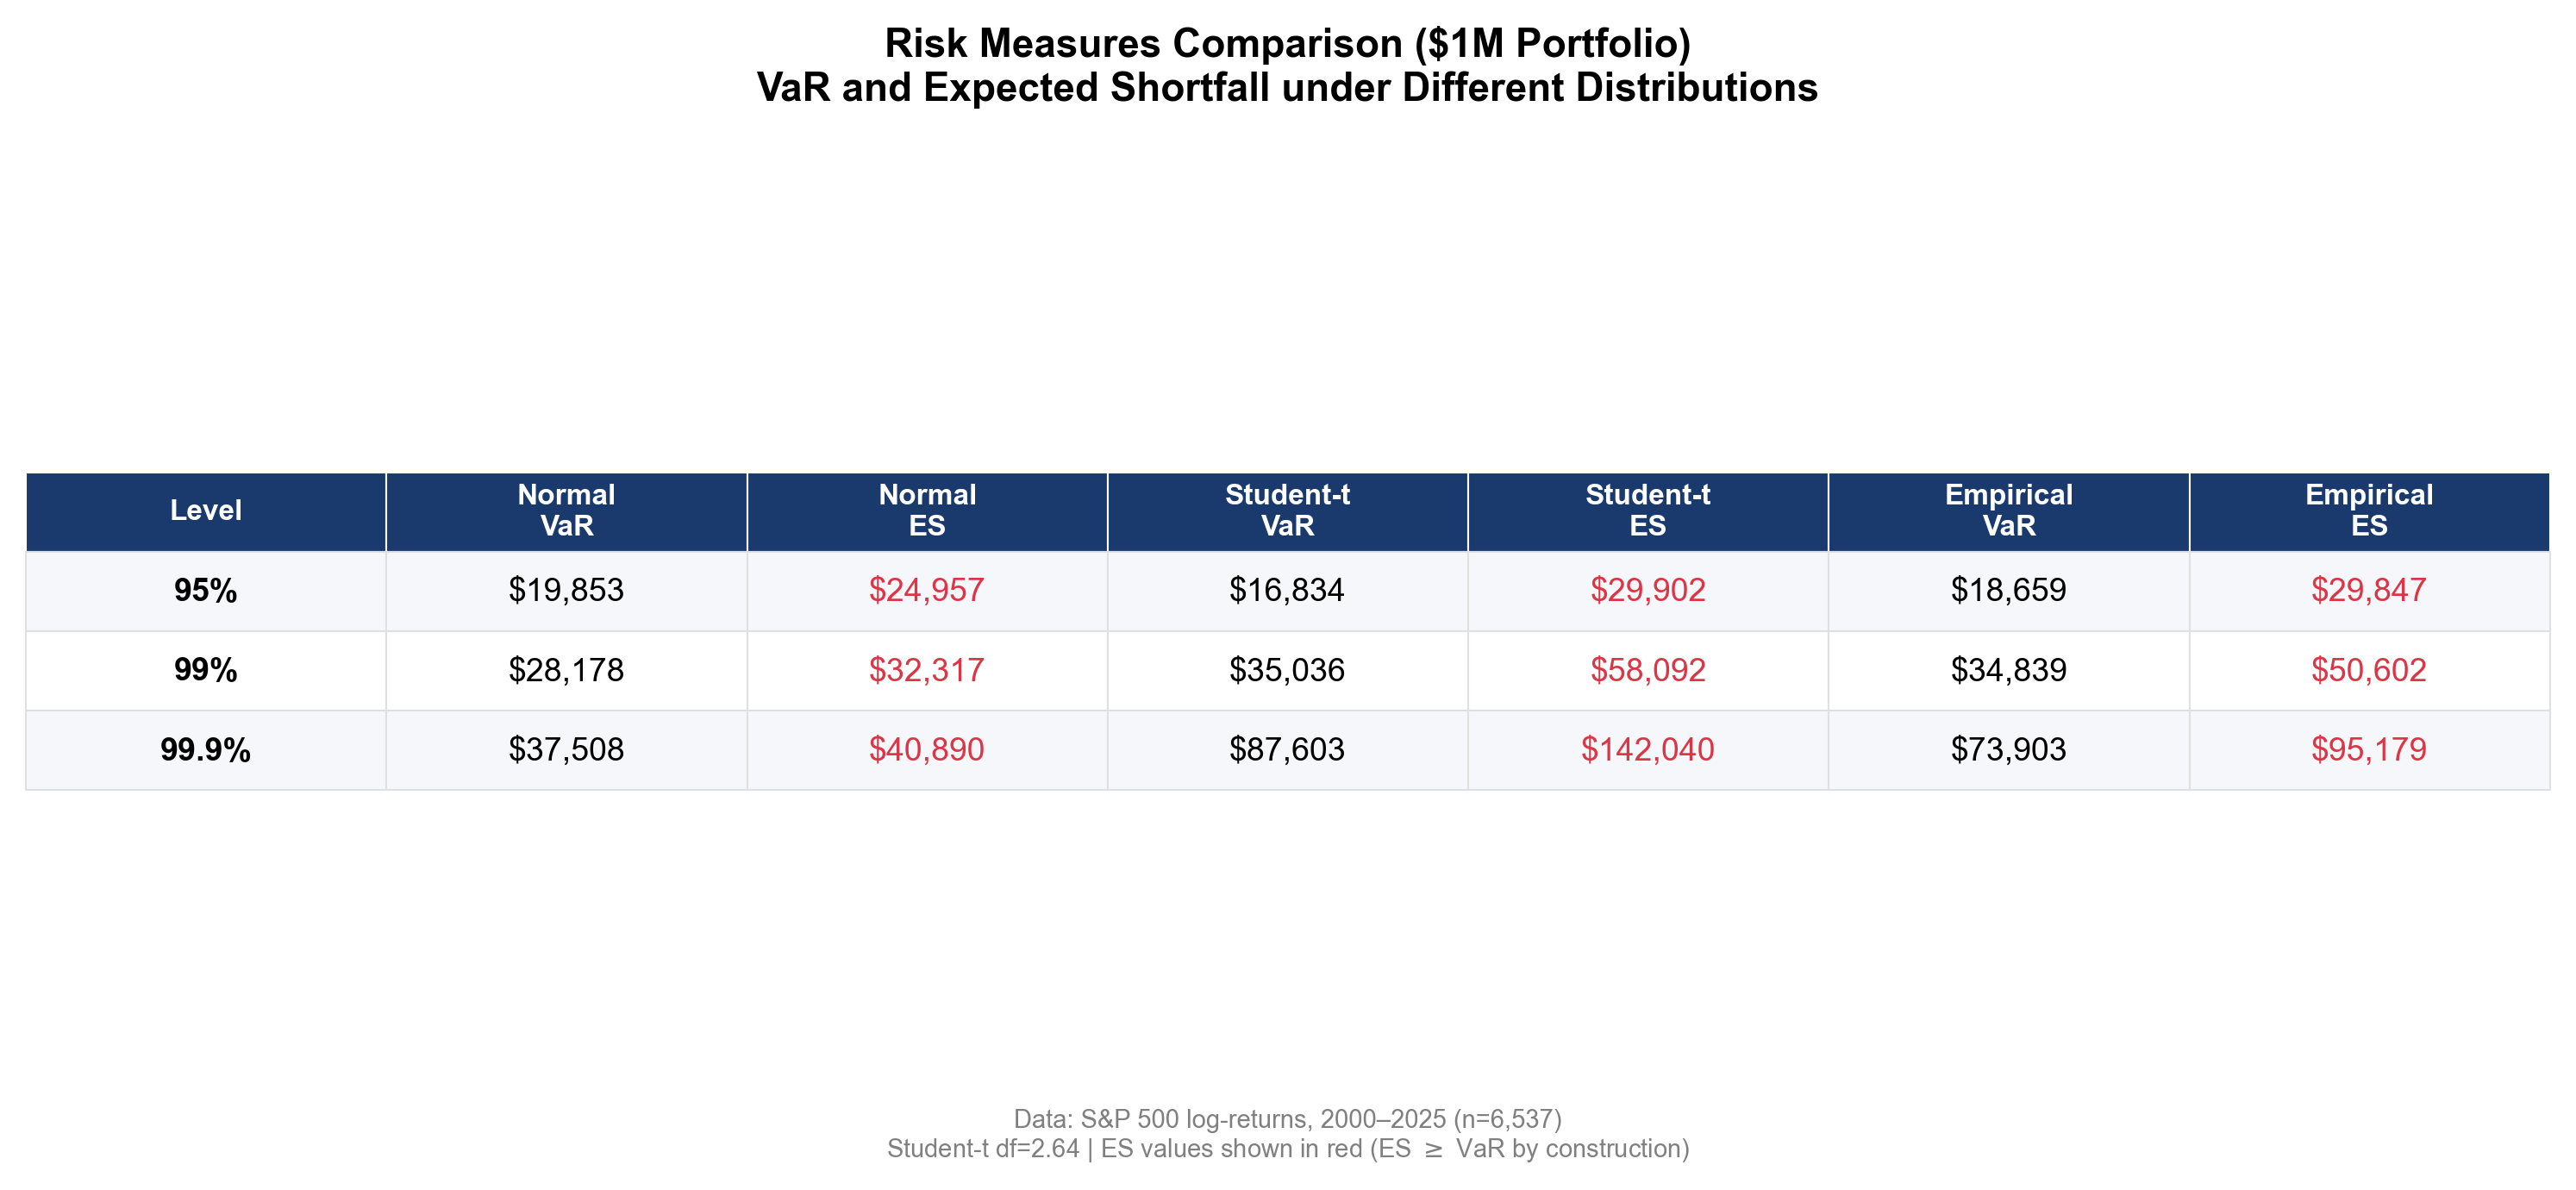
\includegraphics[width=0.72\textwidth]{ch2_risk_comparison_table.png}
\end{center}
\vspace{-0.4cm}
\quantlet{SFM\_ch2\_risk\_comparison}{https://github.com/QuantLet/Stat_fin_markets/tree/master/Ch_02/SFM_ch2_risk_management}
{\footnotesize
\begin{itemize}\setlength{\itemsep}{0pt}
\item Nicio distribuție nu domină pe toate criteriile; Student-$t$: cel mai bun echilibru ajustare/parsimonie
\item EVT: cea mai bună pentru cuantile extreme, dar agnostică față de centru
\end{itemize}}
\end{frame}

%--- PhD Slide 6 ---
\slidelevel{PhD}
\begin{frame}{Testul Vuong și reguli de scor}
\begin{itemize}
\item \textbf{Testul Vuong (1989)}: compararea modelelor neimbricate (\textit{non-nested} --- modele care nu sunt subcazuri unul altuia)
\[
V = \frac{\sum_{i=1}^n m_i}{\sqrt{n}\,\hat{\sigma}_m}, \quad m_i = \ln\frac{f_1(x_i;\hat{\theta}_1)}{f_2(x_i;\hat{\theta}_2)}
\]
$V \sim N(0,1)$ sub $H_0$: modelele sunt echivalente
\item \textbf{CRPS} (Continuous Ranked Probability Score):
\[
\text{CRPS}(F, x) = \int_{-\infty}^{\infty} (F(y) - \mathbf{1}_{y \geq x})^2\,dy
\]
\item Regulă de scor proprie: încurajează previziuni probabilistice oneste
\end{itemize}
\end{frame}

%--- PhD Slide 7 ---
\slidelevel{PhD}
\begin{frame}{Evaluarea densităților predictive}
\begin{itemize}
\item \textbf{Testul Diebold--Mariano (1995)}:
$H_0$: aceeași capacitate predictivă;\quad $H_1$: un model este superior
\[
DM = \frac{\bar{d}}{\sqrt{\widehat{\text{Var}}(\bar{d})/n}} \;\xrightarrow{d}\; N(0,1), \quad d_t = L(e_{1t}) - L(e_{2t})
\]
{\small $L(\cdot)$ = funcție de pierdere (ex.\ pătratică); $e_{it}$ = eroarea de previziune a modelului $i$}
\item \textbf{Validare încrucișată}: evaluare $k$-fold a ajustării distribuționale
\item \textbf{Transformata probabilității integrale (PIT)}:
\begin{itemize}
\item Dacă $F$ este CDF-ul adevărat, atunci $U_i = F(X_i) \sim \text{Uniform}(0,1)$
\item Testarea uniformității valorilor PIT $\Rightarrow$ testarea adecvării distribuționale
\item Transformata Rosenblatt (1952) pentru cazul multivariat
\end{itemize}
\item Ajustarea in-sample $\neq$ capacitatea predictivă out-of-sample
\item Risc de supraajustare: modelele complexe (GH, 5 parametri) pot supraajusta in-sample
\end{itemize}
\end{frame}

%--- PhD Slide 7b ---
\slidelevel{PhD}
\begin{frame}{Testul de echivalență a cozilor}
\begin{defn}[Testul Jansen \& de Vries (1991)]
$H_0$: indicele de coadă (\textit{tail index}) este egal pentru două serii financiare: $\alpha_X = \alpha_Y$.

Statistica de test bazată pe estimatorul Hill:
\[
T = \frac{\hat{\alpha}_{H,X} - \hat{\alpha}_{H,Y}}{\sqrt{\hat{\alpha}_{H,X}^2/k_X + \hat{\alpha}_{H,Y}^2/k_Y}} \xrightarrow{d} N(0,1)
\]
unde $k_X, k_Y$ sunt numerele de ordine statistice folosite.
\end{defn}

\begin{exampleblock}{Aplicație: S\&P 500 vs.\ DAX}
\begin{itemize}
\item $\hat{\alpha}_{H,\text{SP}} = 3{,}2$ ($k = 100$); \;$\hat{\alpha}_{H,\text{DAX}} = 2{,}9$ ($k = 100$)
\item $T = \frac{3{,}2 - 2{,}9}{\sqrt{3{,}2^2/100 + 2{,}9^2/100}} = \frac{0{,}3}{0{,}432} = 0{,}69$; \;$|T| < 1{,}96$ $\Rightarrow$ \textbf{nu respingem} $H_0$
\item Cozile S\&P 500 și DAX au indicele de coadă \textbf{statistic echivalent}
\end{itemize}
\end{exampleblock}

\end{frame}

%--- MSc Slide 7b ---
\slidelevel{MSc}
\begin{frame}{Intervale de încredere pentru estimatorii distribuționali}
\begin{rmk}[Instabilitatea estimatorilor]
\begin{itemize}
\item Estimatorii $\hat{\alpha}_{\text{stabil}}$, $\hat{\nu}_t$, $\hat{\xi}_{\text{Hill}}$ sunt sensibili la dimensiunea eșantionului $n$
\item \textbf{Raportați întotdeauna erori standard, nu doar estimări punctuale!}
\end{itemize}
\end{rmk}

\vspace{0.2cm}
\begin{center}
\renewcommand{\arraystretch}{1.1}
\footnotesize
\begin{tabular}{lccc}
\toprule
\textbf{Estimator} & $n = 500$ & $n = 2{.}500$ & $n = 10{.}000$ \\
\midrule
$\hat{\alpha}_{\text{stabil}}$ & $1{,}70 \pm 0{,}12$ & $1{,}70 \pm 0{,}05$ & $1{,}70 \pm 0{,}03$ \\
$\hat{\nu}_t$ & $5{,}0 \pm 1{,}2$ & $5{,}0 \pm 0{,}5$ & $5{,}0 \pm 0{,}25$ \\
$\hat{\xi}_{\text{Hill}}$ & $0{,}30 \pm 0{,}08$ & $0{,}30 \pm 0{,}04$ & $0{,}30 \pm 0{,}02$ \\
\bottomrule
\end{tabular}
\end{center}

\begin{alertblock}{Implicație practică}
\begin{itemize}
\item Cu $n = 500$, intervalul de încredere pentru $\hat{\nu}_t$ este $[3{,}8;\; 6{,}2]$ --- diferență enormă în VaR!
\item Estimările stabile necesită $n > 2{.}000$ pentru precizie rezonabilă
\end{itemize}
\end{alertblock}
\end{frame}

%--- Y3 Slide 8 ---
\slidelevel{Y3}
\begin{frame}{Exemplu AIC/BIC --- Selecția modelului}
\begin{exampleblock}{Exercițiu}
Ajustăm 4 distribuții pe $n = 2{.}500$ randamente zilnice S\&P~500. Log-verosimilitatea maximă:
\end{exampleblock}

\vspace{0.1cm}
\begin{center}
\renewcommand{\arraystretch}{1.1}
\footnotesize
\begin{tabular}{lcccccc}
\toprule
\textbf{Model} & $k$ & $\hat{\ell}$ & AIC $= -2\hat{\ell} + 2k$ & BIC $= -2\hat{\ell} + k\ln n$ & $\Delta$AIC & $\Delta$BIC \\
\midrule
Normală & 2 & 7{.}420 & $-14{.}836$ & $-14{.}824$ & 294 & 281 \\
Student-$t$ & 3 & 7{.}555 & $-15{.}104$ & $-15{.}086$ & 26 & 19 \\
Student-$t$ asim. & 4 & 7{.}569 & $\mathbf{-15{.}130}$ & $\mathbf{-15{.}105}$ & \textbf{0} & \textbf{0} \\
Stabilă & 4 & 7{.}563 & $-15{.}118$ & $-15{.}093$ & 12 & 12 \\
\bottomrule
\end{tabular}
\end{center}

\begin{block}{Interpretare}
\begin{itemize}
\item $\Delta\text{AIC} > 10$: dovadă puternică \textit{contra} modelului (Burnham \& Anderson)
\item Normală: $\Delta = 294$ (respinsă masiv); Student-$t$ sim.: $\Delta = 26$ (respinsă)
\item \textbf{Student-$t$ asimetrică câștigă} pe AIC și BIC; Stabilă aproape echivalentă ($\Delta = 12$)
\end{itemize}
\end{block}
\end{frame}

%=============================================================================
% SECȚIUNEA 9b: COPULE ȘI DEPENDENȚA DE COADĂ
%=============================================================================
\section{Copule și dependența de coadă}

%--- Y3 Slide 1 ---
\slidelevel{Y3}
\begin{frame}{De la marginale la dependență}
\begin{itemize}
\item Până acum am modelat distribuția \textbf{unui singur activ} (marginală)
\item Riscul de portofoliu depinde de \textbf{cum se mișcă activele împreună} --- structura de dependență
\item Corelația Pearson surprinde doar dependența \textbf{liniară}
\item \textbf{Dependența de coadă}: activele tind să se prăbușească \textit{simultan} în crize
\begin{itemize}
\item În 2008: toate clasele de active au scăzut concomitent
\item Corelația crește exact când diversificarea este cea mai necesară
\end{itemize}
\end{itemize}

\vspace{0.2cm}
\begin{alertblock}{Marginale corecte + copulă greșită = portofoliu greșit}
Două active cu aceleași marginale și aceeași corelație pot avea structuri de dependență extremală \textbf{complet diferite}. Alegerea copulei afectează decisiv estimarea riscului de portofoliu.\\[4pt]
\textbf{Capitolul~4} va trata copulele în detaliu: estimare, selecție, vine copulas și aplicații.
\end{alertblock}
\end{frame}

%--- Y3 Slide 2 ---
\slidelevel{Y3}
\begin{frame}{Teorema lui Sklar --- Intuiție}
\begin{defn}[Copulă --- Intuitiv]
O \textbf{copulă} $C(u,v)$ este o funcție care leagă distribuțiile marginale de distribuția comună. Separă structura de dependență de comportamentul individual al fiecărui activ.
\end{defn}

\begin{thm}[Sklar, 1959]
Orice distribuție bivariată $F(x,y)$ poate fi scrisă ca:
\[
F(x,y) = C\bigl(F_X(x),\; F_Y(y)\bigr)
\]
unde $F_X$, $F_Y$ sunt marginalele, iar $C$ este copula (unică dacă marginalele sunt continue).
\end{thm}

\begin{itemize}
\item \textbf{Pas 1}: Modelăm fiecare activ separat (marginalele --- capitolul actual)
\item \textbf{Pas 2}: Modelăm dependența prin copulă (\textbf{Capitolul~4})
\item Aceasta permite combinații flexibile: marginale Student-$t$ + copulă Clayton
\end{itemize}
\end{frame}

%--- MSc Slide 3 ---
\slidelevel{MSc}
\begin{frame}{Familii de copule și dependența de coadă}
\begin{center}
\renewcommand{\arraystretch}{1.2}
\footnotesize
\begin{tabular}{lcccl}
\toprule
\textbf{Copulă} & \textbf{Param.} & $\lambda_L$ (coadă inf.) & $\lambda_U$ (coadă sup.) & \textbf{Utilizare} \\
\midrule
Gaussiană & $\rho$ & 0 & 0 & Benchmark \\
Student-$t$ & $\rho, \nu$ & $>0$ & $>0$ & Riscul de coadă simetric \\
Clayton & $\theta$ & $>0$ & 0 & Prăbușiri comune \\
Gumbel & $\theta$ & 0 & $>0$ & Co-mișcări pozitive \\
Frank & $\theta$ & 0 & 0 & Dependență simetrică \\
\bottomrule
\end{tabular}
\end{center}

\begin{itemize}
\item \textbf{Coeficientul de dependență de coadă (\textit{tail dependence})}: $\lambda_L = \lim_{u\to 0} P(U \leq u \mid V \leq u)$
\item Copulă Gaussiană: $\lambda_L = \lambda_U = 0$ chiar dacă $\rho = 0{,}9$ --- \textbf{subestimează} riscul de prăbușire comună
\item Copulă Student-$t$: $\lambda_L = \lambda_U = 2\,t_{\nu+1}\!\left(-\sqrt{(\nu+1)(1-\rho)/(1+\rho)}\right) > 0$
\item \textbf{Lecție}: Corelația mare $\neq$ dependență de coadă puternică
\end{itemize}
\end{frame}

%--- PhD Slide 4 ---
\slidelevel{PhD}
\begin{frame}{Implicații pentru managementul riscului de portofoliu}
\begin{itemize}
\item \textbf{VaR de portofoliu sub diferite copule}:
\begin{itemize}
\item Copulă Gaussiană $\Rightarrow$ VaR de portofoliu mai mic (subestimează riscul comun)
\item Copulă Student-$t$ $\Rightarrow$ VaR mai mare (captează prăbușiri simultane)
\item Diferența crește dramatic pentru cuantile extreme ($< 0{,}1\%$)
\end{itemize}
\item \textbf{Basel III}: cere modele de dependență de coadă pentru portofolii de tranzacționare
\item \textbf{Estimare}: pseudo-MLE (Joe, 1997); inversiunea rangurilor $\hat{u}_i = R_i/(n+1)$
\item \textbf{Selecția copulei}: AIC/BIC pe funcția de verosimilitate a copulei
\item \textbf{Vine copulae} (Aas et al., 2009): extensie la dimensiuni mari prin descompunere pair-copula
\end{itemize}

\begin{rmk}
\begin{itemize}
\item Capitolul 4 va trata copulele în detaliu. Aici reținem: \textbf{marginale corecte + copulă greșită = risc de portofoliu greșit}
\end{itemize}
\end{rmk}
\end{frame}


%=============================================================================
% TITLU PARTEA II
%=============================================================================
% SECȚIUNEA 10: IMPLICAȚII PENTRU MANAGEMENTUL RISCULUI
%=============================================================================
\section{Implicații pentru managementul riscului}

%--- Y3 Slide 1 ---
\slidelevel{Y3}
\begin{frame}{Întrebarea de risc}
\begin{itemize}
\item O bancă deține un portofoliu în valoare de \$1.000.000
\item Întrebarea fundamentală: \textit{,,Care este pierderea maximă pe care o putem aștepta într-o zi dată, cu un nivel specificat de încredere?''}
\item \textbf{Intuiția cuantilei}: cuantila de ordin $\alpha$ $q_\alpha$ satisface:
\[
P(r_t \leq q_\alpha) = \alpha
\]
\item Pentru $\alpha = 0{,}01$: $q_{0{,}01}$ este depășit (la scădere) doar 1\% din timp
\item În 100 de zile de tranzacționare, ne așteptăm să pierdem mai mult decât $q_{0{,}01}$ în $\approx 1$ zi
\end{itemize}
\end{frame}

%--- Y3 Slide 2 ---
\slidelevel{Y3}
\begin{frame}{Value-at-Risk --- Convenții de semn și proprietăți}
{\small\textit{Definiția de lucru a fost introdusă în Secțiunea~4. Aici studiem convențiile și limitările.}}
\vspace{0.1cm}
\begin{itemize}
\item Cu probabilitatea $(1-\alpha)$, pierderea zilnică \textbf{nu va depăși} $\text{VaR}_\alpha = -F^{-1}(\alpha)$
\item \textbf{Convenție}: ,,VaR 1\%'' înseamnă $\alpha = 0{,}01$ (pierdere depășită cu probabilitate 1\%)
\item Semnul minus convertește cuantila negativă într-o sumă pozitivă de pierdere
\end{itemize}

\begin{alertblock}{Convenție de semn --- atenție!}
\begin{itemize}
\item \textbf{Secțiunile 2--8}: $\text{VaR}_\alpha = -F^{-1}(\alpha)$ --- cuantila cu semn schimbat (rezultat pozitiv)
\item \textbf{Secțiunea EVT}: $u$ și VaR sunt magnitudini de pierdere (pozitive)
\item Ambele convenții dau \textbf{aceeași valoare numerică}
\end{itemize}
\end{alertblock}
\end{frame}

%--- Y3 Slide 3 ---
\slidelevel{Y3}
\begin{frame}{VaR sub ipoteza normală}
\begin{itemize}
\item Dacă $r_t \sim N(\mu, \sigma^2)$:
\[
\text{VaR}_\alpha = -(\mu + \sigma \cdot z_\alpha), \quad z_\alpha = \Phi^{-1}(\alpha)
\]
\item \textbf{Exemplu}: $\mu = 0$, $\sigma = 0{,}015$, portofoliu = \$1M, $\alpha = 0{,}01$:
\[
\text{VaR}_{0{,}01} = -0{,}015 \times (-2{,}326) \times 1.000.000 = \$34.890
\]
\item În 99 din 100 de zile de tranzacționare, pierderea nu va depăși \$34.890
\end{itemize}

\begin{center}
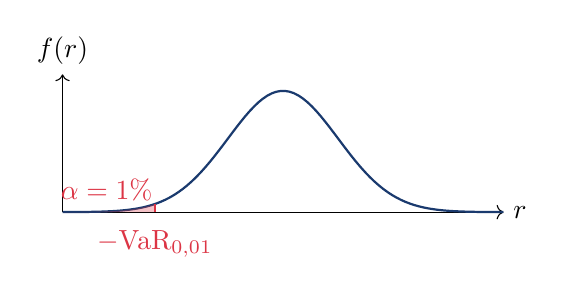
\begin{tikzpicture}[scale=0.7]
\draw[->] (-4,0) -- (4,0) node[right] {$r$};
\draw[->] (-4,0) -- (-4,2.5) node[above] {$f(r)$};
\draw[MainBlue, thick, domain=-4:4, samples=100] plot (\x, {2.2*exp(-\x*\x/2)});
\fill[Crimson, opacity=0.3, domain=-4:-2.326, samples=50] plot (\x, {2.2*exp(-\x*\x/2)}) -- (-2.326,0) -- (-4,0) -- cycle;
\draw[Crimson, thick, dashed] (-2.326,0) -- (-2.326,{2.2*exp(-2.326*2.326/2)});
\node[below, Crimson] at (-2.326,-0.15) {$-\text{VaR}_{0{,}01}$};
\node[Crimson] at (-3.2,0.4) {$\alpha = 1\%$};
\end{tikzpicture}
\end{center}
\end{frame}

%--- Y3 Slide 4 ---
\slidelevel{Y3}
\begin{frame}{De ce contează distribuția pentru VaR}
\begin{center}
\renewcommand{\arraystretch}{1.1}
\footnotesize
\begin{tabular}{l c c c}
\toprule
\textbf{Model} & \textbf{VaR 1\% (\$1M)} & \textbf{VaR 0{,}1\% (\$1M)} & \textbf{Raport față de normală} \\
\midrule
Normală & \$27.000 & \$35.900 & 1{,}0$\times$ \\
Student-$t$ ($\nu=5$) & \$33.700 & \$58.400 & 1{,}6$\times$ \\
Stabilă ($\alpha=1{,}7$) & \$41.000 & \$90.200 & 2{,}5$\times$ \\
\bottomrule
\end{tabular}
\end{center}

\begin{itemize}
\item La 1\%: diferență moderată ($\sim$25\%); la 0{,}1\%: \textbf{dramatică} (1{,}6--2{,}5$\times$)
\item \textbf{Concluzie}: Alegerea distribuției afectează direct capitalul necesar
\item Distribuția stabilă necesită capital de $2{,}5\times$ mai mare decât cea normală la cuantila 0{,}1\%
\end{itemize}
\end{frame}

%--- Y3 Slide 4b ---
\slidelevel{Y3}
\begin{frame}{VaR sub diferite distribuții --- Vizualizare}
\begin{center}
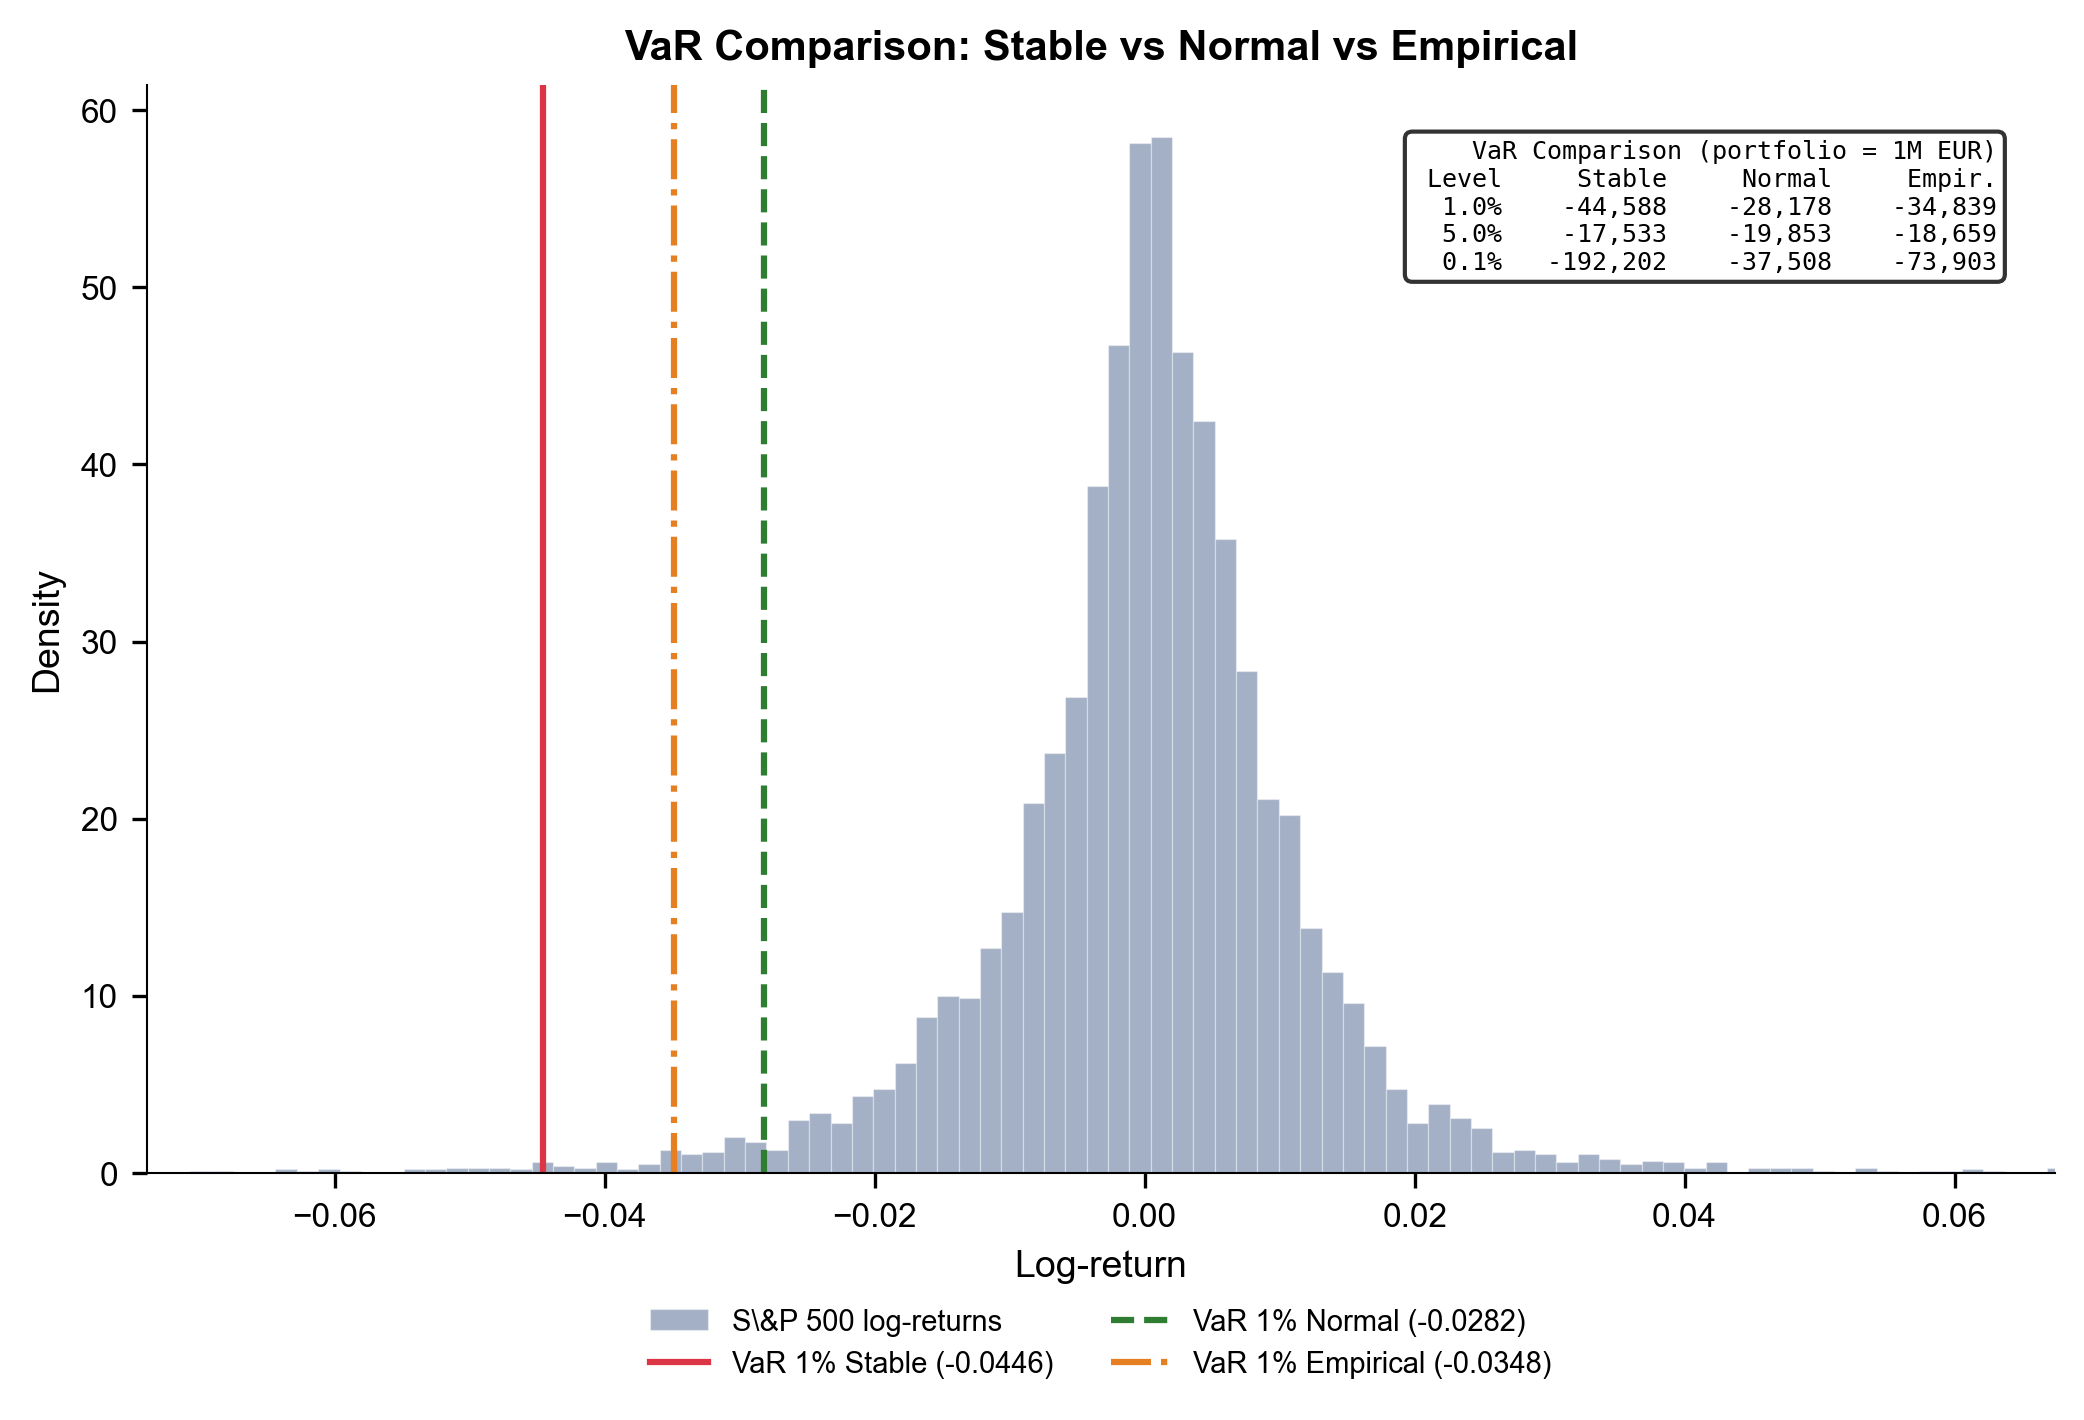
\includegraphics[width=0.5\textwidth]{ch2_var_comparison.png}
\end{center}
\quantlet{SFM\_ch2\_var\_comparison}{https://github.com/QuantLet/Stat_fin_markets/tree/master/Ch_02/SFM_ch2_risk_management}
\vspace{-0.2cm}
\begin{itemize}
\item Divergența cozilor crește dramatic cu nivelul de încredere
\item La 0{,}1\%, distribuția normală subestimează riscul cu \textbf{peste 60\%} (Student-$t$) și \textbf{150\%} (stabilă)
\item Cerințele de capital Basel depind critic de ipoteza distribuțională
\end{itemize}
\end{frame}

%--- Y3 Slide 5 ---
\slidelevel{Y3}
\begin{frame}{Limitările VaR}
\begin{itemize}
\item VaR ne spune \textit{pragul} celei mai rele fracțiuni $\alpha$ din zile
\item Dar \textbf{nu} cât de rău devine lucrurile \textit{dincolo} de acel prag
\item VaR nu distinge între ,,pierderea de \$35k'' și ,,pierderea de \$200k'' --- ambele sunt ,,depășiri VaR''
\item O măsură mai bună (\textbf{Expected Shortfall}) rezolvă această limitare
\end{itemize}

\vspace{0.3cm}
\begin{alertblock}{VaR nu este subaditivă}
\begin{itemize}
\item Diversificarea poate \textit{crește} VaR: $\text{VaR}(X+Y) > \text{VaR}(X) + \text{VaR}(Y)$ este posibil
\item Acest lucru contrazice principiul că diversificarea reduce riscul
\end{itemize}
\end{alertblock}
\end{frame}

%--- Y3 Slide 5b ---
\slidelevel{Y3}
\begin{frame}{VaR vs.\ ES --- Subaditivitate vizuală}
\begin{center}
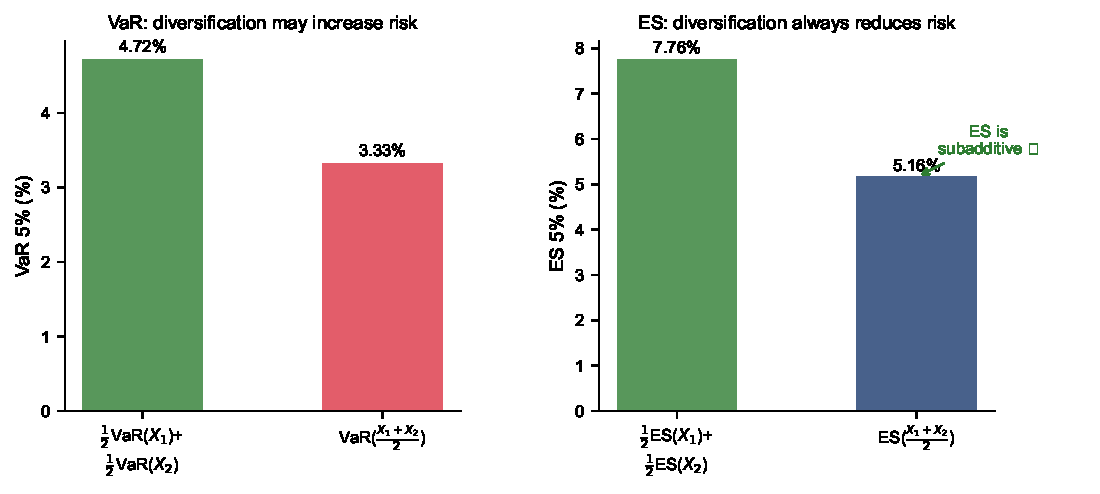
\includegraphics[width=0.75\textwidth]{ch2_var_subadditivity.pdf}
\end{center}
\quantlet{SFM\_ch2\_var\_subadditivity}{https://github.com/QuantLet/Stat_fin_markets/tree/master/Ch_02/SFM_ch2_risk_management}
\vspace{-0.2cm}
\begin{itemize}
\item Stânga: VaR a portofoliului poate depăși suma VaR-urilor individuale (non-subaditivă)
\item Dreapta: ES a portofoliului este \textbf{întotdeauna} $\leq$ suma ES-urilor (subaditivă, coerentă)
\end{itemize}
\end{frame}

%--- MSc Slide 6 ---
\slidelevel{MSc}
\begin{frame}{Expected Shortfall}
\begin{defn}[Expected Shortfall]
\textbf{Expected Shortfall} (CVaR) la nivelul $\alpha$:
\[
\text{ES}_\alpha = -\frac{1}{\alpha}\int_0^\alpha F^{-1}(p)\,dp \stackrel{F \text{ cont.}}{=} \E[-X \mid X \leq -\text{VaR}_\alpha].
\]
Egalitatea cu așteptarea condiționată vale pentru distribuții \textbf{continue}.
\end{defn}

\begin{itemize}
\item \textbf{Interpretare}: pierderea medie dat fiind că suntem în cele mai rele $\alpha\%$ din zile
\item Sub normalitate: $\text{ES}_\alpha = -\mu + \sigma\frac{\phi(\Phi^{-1}(\alpha))}{\alpha}$
\item ES este o măsură \textbf{coerentă} de risc (subaditivă):
\[
\text{ES}(X+Y) \leq \text{ES}(X) + \text{ES}(Y)
\]
\item Diversificarea reduce întotdeauna ES (spre deosebire de VaR)
\end{itemize}
\end{frame}

%--- MSc Slide 6b ---
\slidelevel{MSc}
\begin{frame}{Axiomele coerență --- Artzner et al.\ (1999)}
\begin{defn}[Măsură coerentă de risc]
O funcțională $\rho: \mathcal{X} \to \R$ este o \textbf{măsură coerentă de risc (\textit{coherent risk measure})} dacă satisface:
\end{defn}
\begin{enumerate}
\item[\textcolor{MainBlue}{\textbf{A1.}}] \textbf{Monotonie}: $X \leq Y \Rightarrow \rho(X) \geq \rho(Y)$
\begin{itemize}
\item Pierderi mai mari $\Rightarrow$ risc mai mare
\end{itemize}
\item[\textcolor{MainBlue}{\textbf{A2.}}] \textbf{Subaditivitate}: $\rho(X+Y) \leq \rho(X) + \rho(Y)$
\begin{itemize}
\item Diversificarea nu crește riscul
\end{itemize}
\item[\textcolor{MainBlue}{\textbf{A3.}}] \textbf{Omogenitate pozitivă}: $\rho(\lambda X) = \lambda\rho(X)$, $\lambda > 0$
\begin{itemize}
\item Dublarea poziției dublează riscul
\end{itemize}
\item[\textcolor{MainBlue}{\textbf{A4.}}] \textbf{Invarianță la translație}: $\rho(X + c) = \rho(X) - c$
\begin{itemize}
\item Adăugarea de numerar reduce riscul cu aceeași sumă
\end{itemize}
\end{enumerate}
\vspace{0.2cm}
\begin{alertblock}{Rezultat cheie}
\begin{itemize}
\item \textbf{ES este coerentă} (satisface A1--A4); \textbf{VaR nu este} (eșuează la A2)
\end{itemize}
\end{alertblock}
\end{frame}

%--- MSc Slide 7 ---
\slidelevel{MSc}
\begin{frame}{Backtesting VaR --- Testele Kupiec și Christoffersen}
\begin{block}{Testul Kupiec (1995) --- acoperire necondiționată}
$H_0$: rata depășirilor $= \alpha$ \quad vs.\ $H_1$: rata depășirilor $\neq \alpha$
\[
LR_{uc} = -2\ln\frac{\alpha^x(1-\alpha)^{n-x}}{\hat{p}^{\,x}(1-\hat{p})^{n-x}} \;\sim\; \chi^2(1), \quad \hat{p} = x/n
\]
\end{block}
\vspace{-0.1cm}
\begin{block}{Testul Christoffersen (1998) --- independența depășirilor}
$H_0$: depășirile sunt independente \quad vs.\ $H_1$: depășirile se clusterizează
\[
LR_{ind} = -2\ln\frac{\hat{p}^{\,n_1}(1-\hat{p})^{n_0}}{\hat{p}_{01}^{n_{01}}(1-\hat{p}_{01})^{n_{00}}\hat{p}_{11}^{n_{11}}(1-\hat{p}_{11})^{n_{10}}} \;\sim\; \chi^2(1)
\]
{\small $n_{ij}$ = tranzițiile de la starea $i$ la $j$;\; $\hat{p}_{ij} = n_{ij}/(n_{i0}+n_{i1})$}
\end{block}
\vspace{-0.1cm}
{\small \textbf{Test combinat}: $LR_{cc} = LR_{uc} + LR_{ind} \sim \chi^2(2)$.\quad \textbf{Basel III/IV}: de la VaR 1\% (10 zile) la ES 2{,}5\%.}
\end{frame}

%--- MSc Slide 7b ---
\slidelevel{MSc}
\begin{frame}{Backtesting --- Vizualizare}
\begin{center}
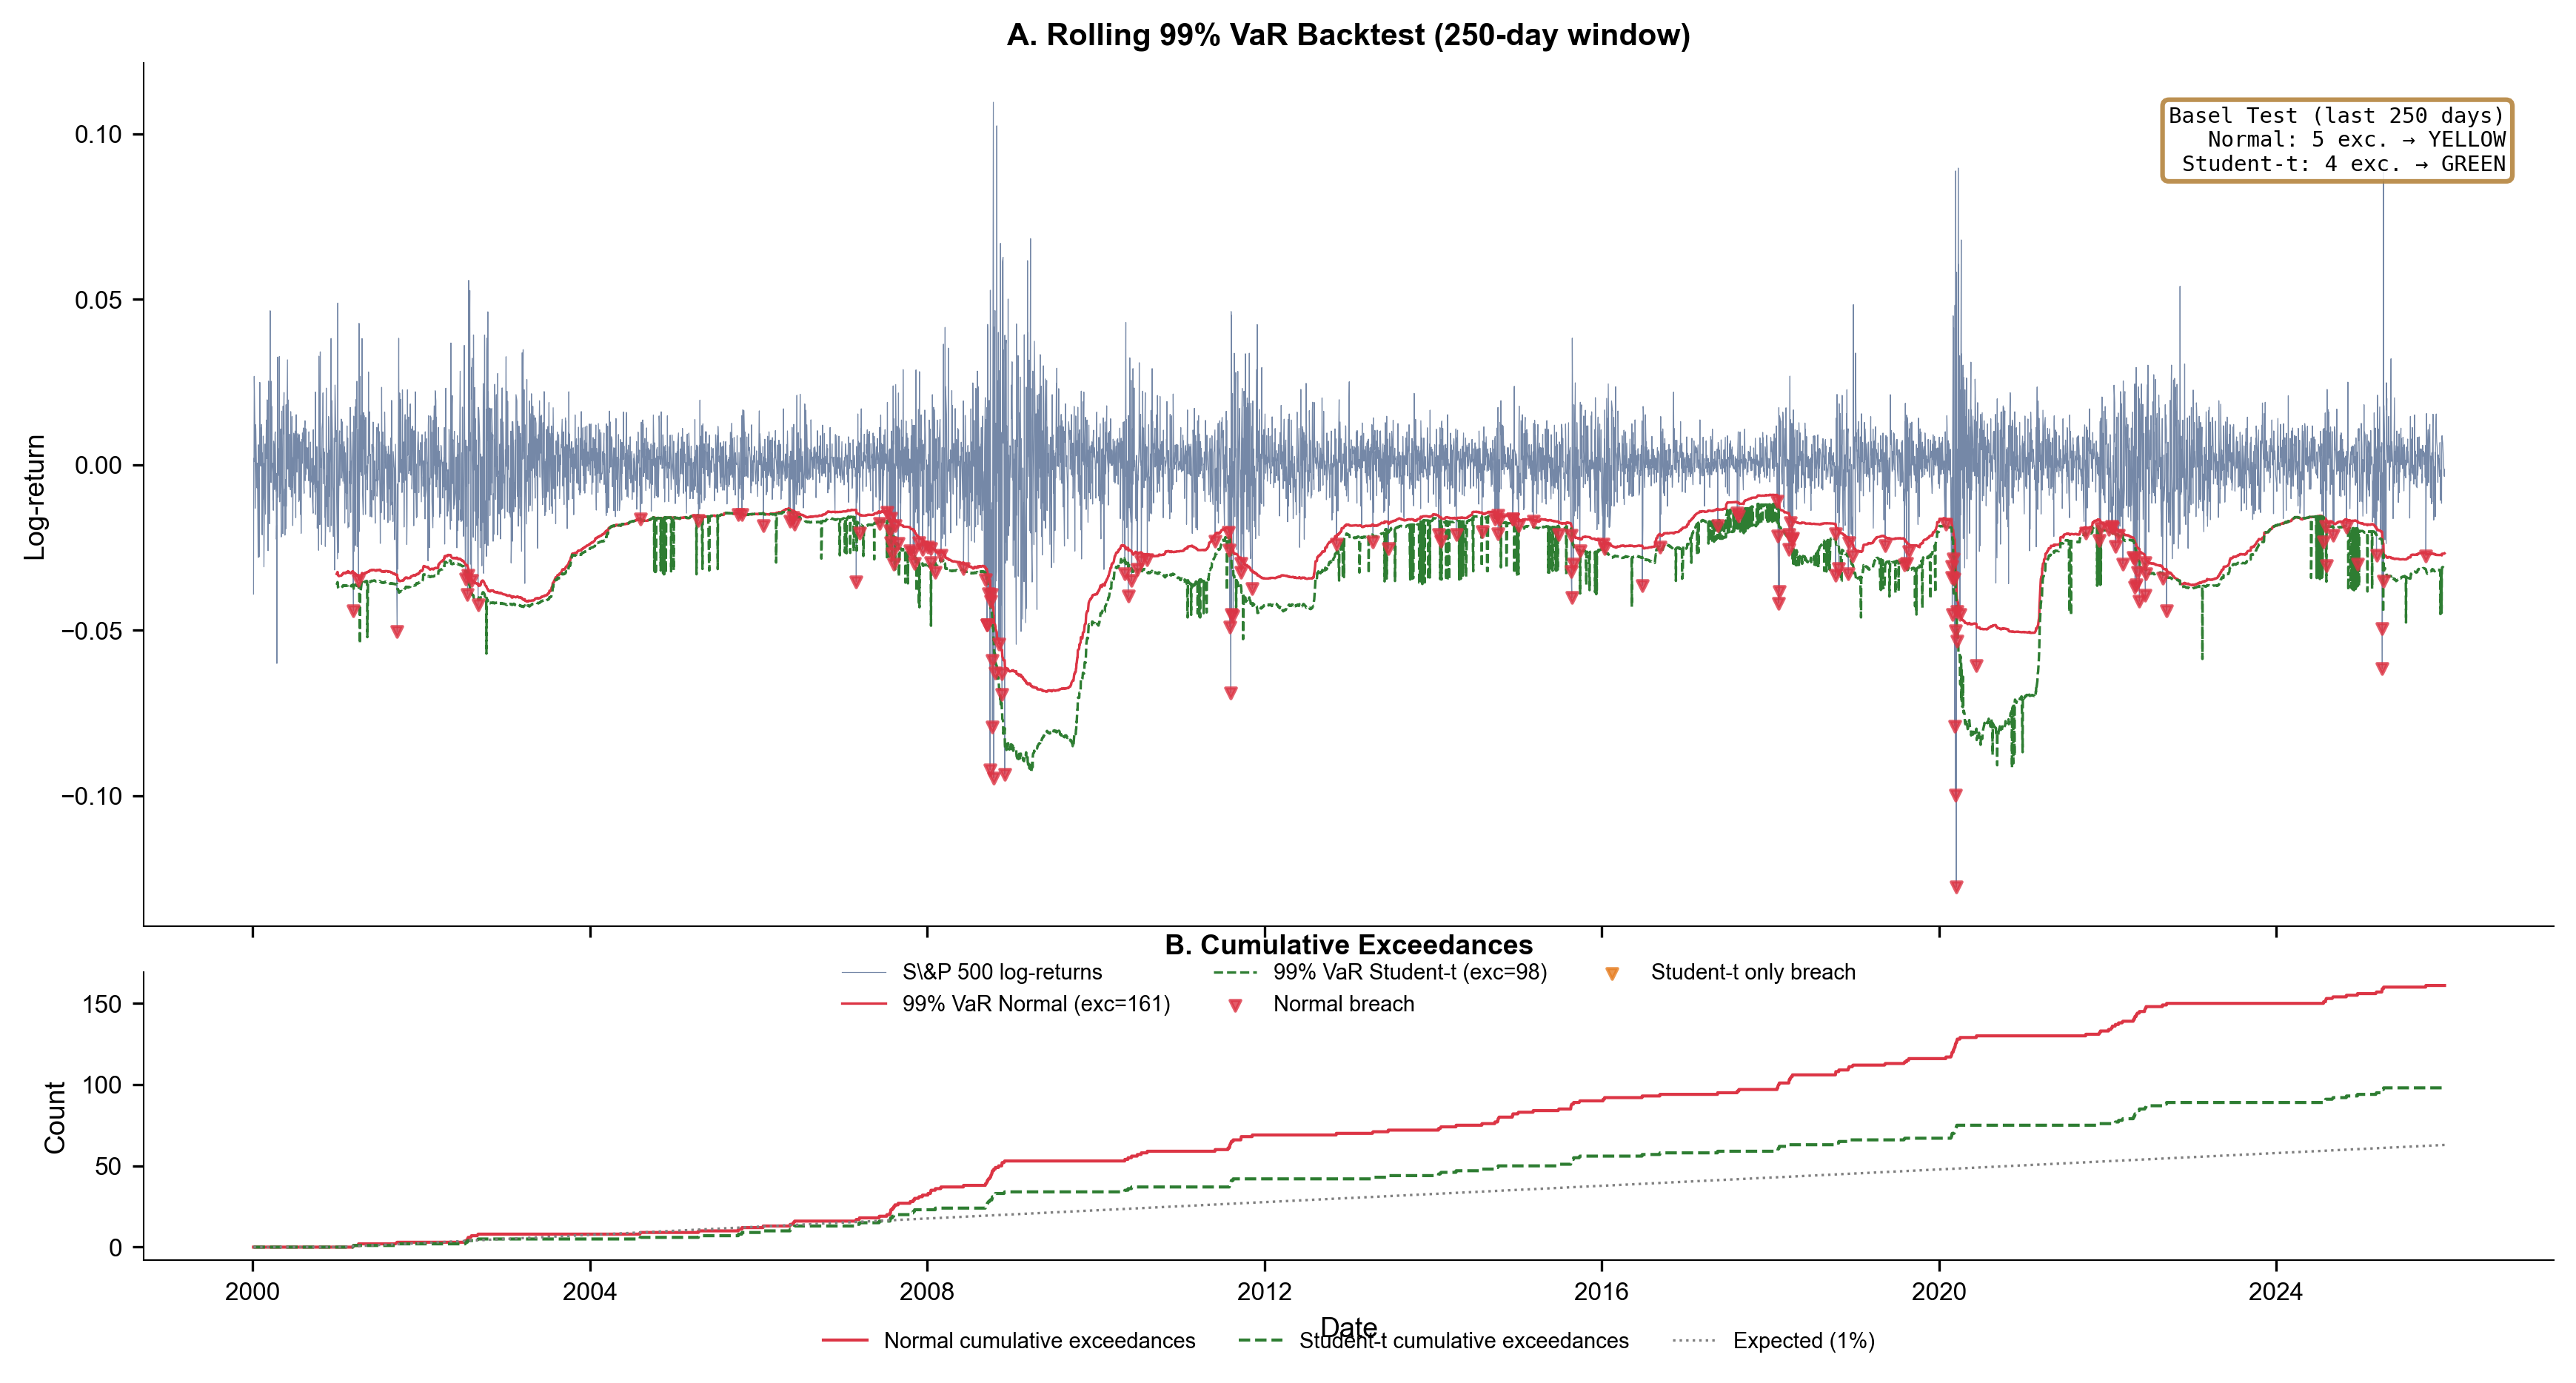
\includegraphics[width=0.52\textwidth]{ch2_var_backtest.png}
\end{center}
\quantlet{SFM\_ch2\_backtest}{https://github.com/QuantLet/Stat_fin_markets/tree/master/Ch_02/SFM_ch2_risk_management}
\vspace{-0.2cm}
\begin{itemize}
\item Semafor Basel: Verde (0--4 depășiri), Galben (5--9), Roșu (10+) per 250 zile
\item Normală: prea multe depășiri $\Rightarrow$ respinsă de Kupiec
\end{itemize}
\end{frame}

%--- MSc Slide 8 ---
\slidelevel{MSc}
\begin{frame}{Rezultate backtest VaR}
\begin{center}
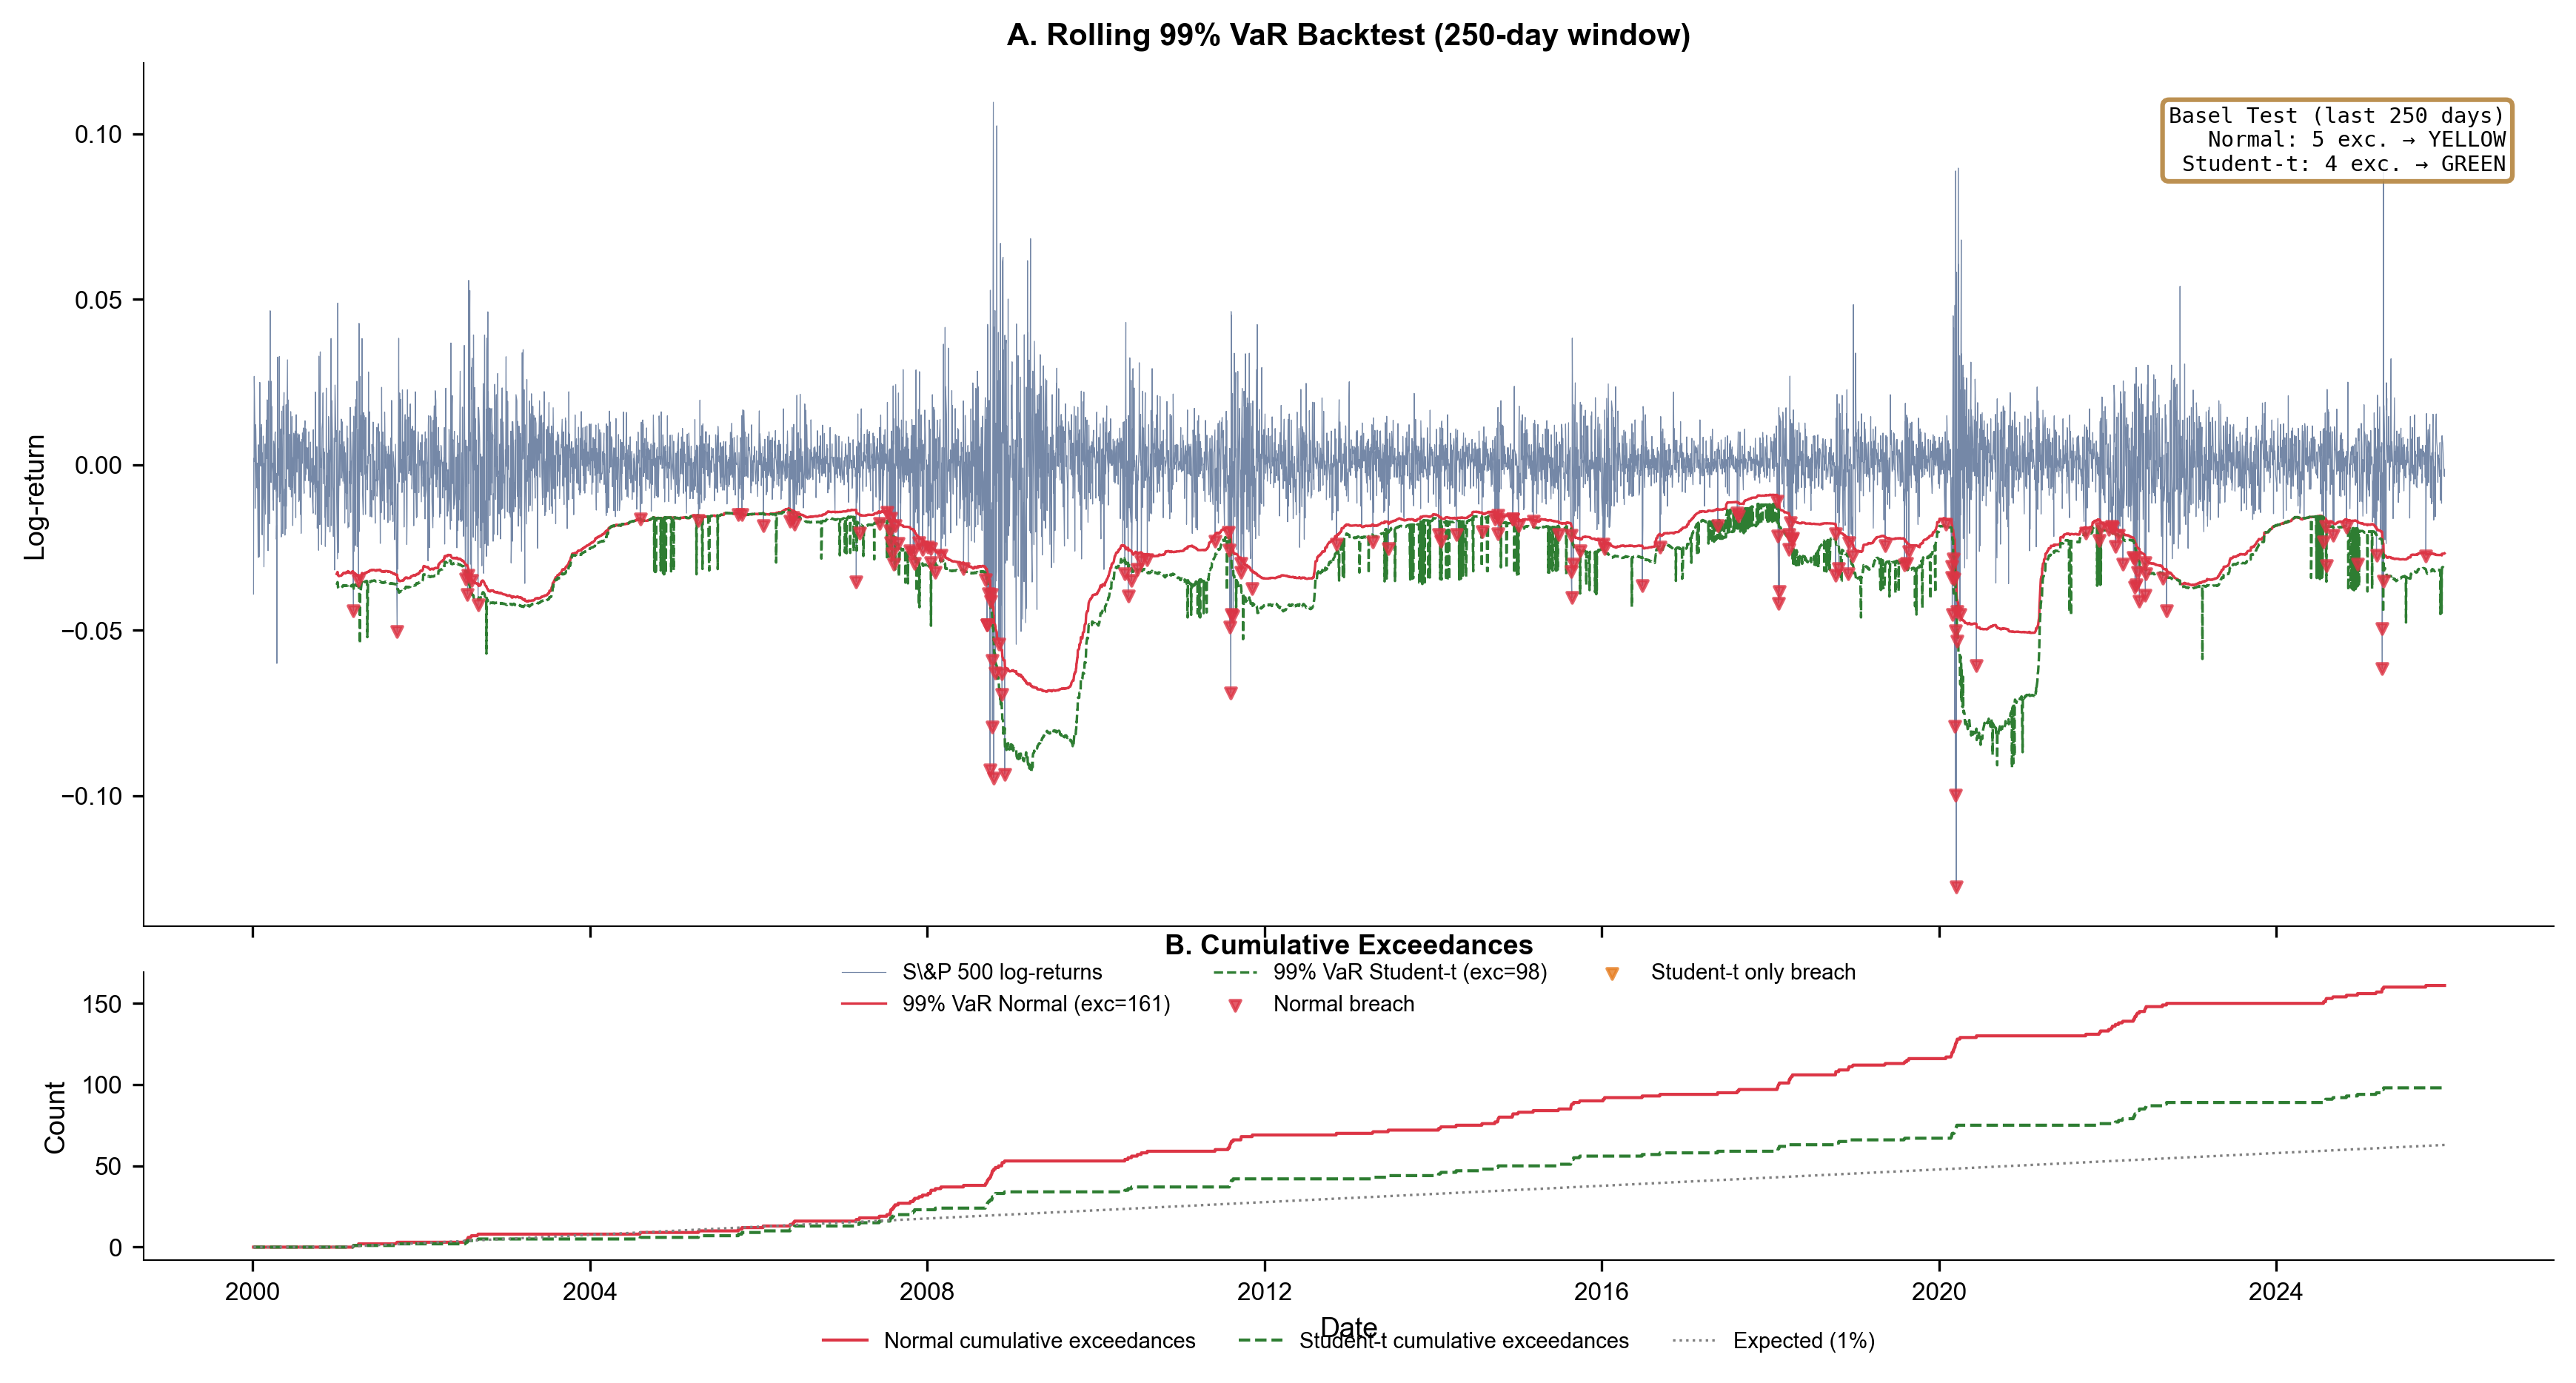
\includegraphics[width=0.58\textwidth]{ch2_var_backtest.png}
\end{center}
\vspace{-0.3cm}
\quantlet{SFM\_ch2\_backtest\_results}{https://github.com/QuantLet/Stat_fin_markets/tree/master/Ch_02/SFM_ch2_risk_management}
{\small
\begin{itemize}\setlength{\itemsep}{0pt}
\item Normală: prea multe depășiri VaR $\Rightarrow$ respinsă de Kupiec
\item Student-$t$: depășiri aproape de rata așteptată; EVT: conservator dar robust
\item \textbf{Riscul de model}: rezervele de capital depind de modelul ales
\end{itemize}}
\end{frame}

%--- PhD Slide 9 ---
\slidelevel{PhD}
\begin{frame}{Măsuri spectrale de risc și elicitabilitate}
\begin{itemize}
\item \textbf{Măsuri spectrale de risc}:
\[
\rho_\phi(X) = -\int_0^1 \phi(p)\,F^{-1}(p)\,dp
\]
cu spectrul de risc $\phi(p) \geq 0$, $\int_0^1 \phi(p)\,dp = 1$, $\phi$ nedescrescătoare
\item VaR: $\phi(p) = \delta(p - \alpha)$; \quad ES: $\phi(p) = \frac{1}{\alpha}\mathbf{1}_{p \leq \alpha}$
\item \textbf{Elicitabilitate} (Gneiting, 2011):
\begin{itemize}
\item VaR este elicitabilă: optimală sub pierderea cuantilică $\rho(x,q) = (\alpha - \mathbf{1}_{x<q})(x-q)$
\item ES \textbf{nu} este elicitabilă singură
\item (VaR, ES) este elicitabilă conjunct (Fissler \& Ziegel, 2016)
\end{itemize}
\end{itemize}
\end{frame}

%--- PhD Slide 9b ---
\slidelevel{PhD}
\begin{frame}{Funcțiile spectrale de risc --- Vizualizare}
\begin{center}
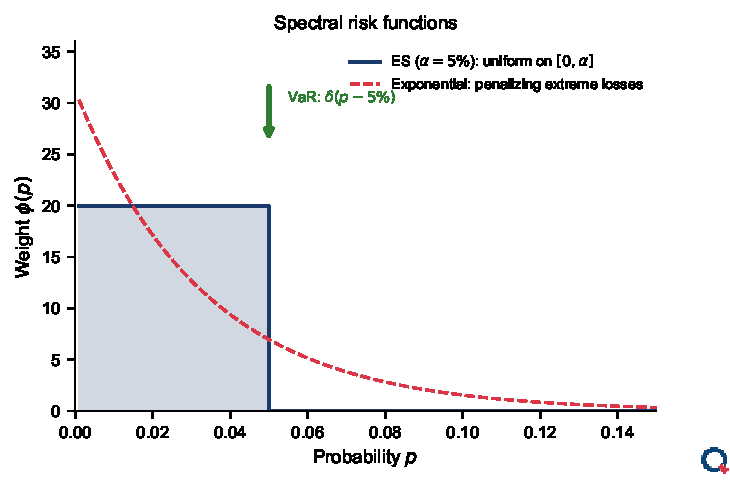
\includegraphics[width=0.5\textwidth]{ch2_spectral_weights.pdf}
\end{center}
\quantlet{SFM\_ch2\_spectral}{https://github.com/QuantLet/Stat_fin_markets/tree/master/Ch_02/SFM_ch2_risk_management}
\begin{itemize}
\item VaR: pondere concentrată într-un singur punct ($\delta$ la $p = \alpha$) --- ignoră ce se întâmplă dincolo
\item ES: pondere uniformă pe $[0, \alpha]$ --- media tuturor pierderilor din coada de $\alpha\%$
\item Spectrul exponențial: penalizează mai mult pierderile cele mai extreme
\end{itemize}
\end{frame}

%--- PhD Slide 10 ---
\slidelevel{PhD}
\begin{frame}{Alocarea capitalului și riscul de model}
\begin{itemize}
\item \textbf{Alocarea Euler}: alocăm ES-ul portofoliului pe pozițiile individuale:
\[
\text{ES}_i = \E[-X_i \mid X_{\text{total}} \leq -\text{VaR}_\alpha]
\]
\item Ipotezele distribuționale afectează direct capitalul alocat per departament
\item \textbf{Distribuții stabile și riscul extrem}: ES sub distribuții stabile diverge pe măsură ce $\alpha \to 0$ mai rapid decât sub Student-$t$
\item \textbf{Cuantificarea riscului de model}: calculăm VaR/ES sub mai multe modele; intervalul cuantifică incertitudinea modelului
\item Răspunsul reglementator: VaR stresat, suplimente de risc de model
\end{itemize}
\end{frame}

%--- MSc Slide 10a ---
\slidelevel{MSc}
\begin{frame}{VaR cu fereastră mobilă (\textit{rolling window})}
\begin{defn}[Rolling VaR]
La momentul $t$, estimăm parametrii $\hat{\theta}_t$ pe fereastra $\{r_{t-W+1}, \ldots, r_t\}$ de lungime $W$ (tipic $W = 250$ zile $\approx$ 1 an). VaR-ul \emph{out-of-sample} pentru ziua $t+1$:
\[
\widehat{\text{VaR}}_{\alpha,t+1} = -F^{-1}(\alpha;\, \hat{\theta}_t)
\]
\end{defn}

\begin{itemize}
\item \textbf{Procedura}: La fiecare zi $t$, fereastra alunecă cu o observație; parametrii se re-estimează
\item \textbf{VaR parametric} (Normal, Student-$t$): $\hat{\theta}_t = (\hat{\mu}_t, \hat{\sigma}_t, [\hat{\nu}_t])$
\item \textbf{VaR istoric} (neparametric): $\widehat{\text{VaR}}_{\alpha,t+1} = -r_{(\lceil \alpha W \rceil)}$ --- cuantila empirică a ferestrei
\item \textbf{Backtest}: comparăm $r_{t+1}$ cu $-\widehat{\text{VaR}}_{\alpha,t+1}$; dacă $r_{t+1} < -\widehat{\text{VaR}}$, avem o depășire (\textit{exceedance})
\item Proporția depășirilor $\hat{p} = x/n$ ar trebui să fie $\approx \alpha$; testăm cu Kupiec/Christoffersen
\end{itemize}
\end{frame}

%--- MSc Slide 10b ---
\slidelevel{MSc}
\begin{frame}{Backtest out-of-sample --- Compararea modelelor}
\begin{exampleblock}{Exercițiu: Fereastră mobilă 250 zile, VaR 1\%, S\&P 500 (2010--2025)}
\begin{center}
\renewcommand{\arraystretch}{1.1}
\footnotesize
\begin{tabular}{lccc}
\toprule
\textbf{Model} & \textbf{Depășiri așteptate} & \textbf{Depășiri reale} & \textbf{$p$-value Kupiec} \\
\midrule
Normal & 37 & 58 & 0{,}001 \\
Student-$t$ ($\nu = 5$) & 37 & 41 & 0{,}42 \\
Stabilă ($\alpha = 1{,}7$) & 37 & 34 & 0{,}55 \\
EVT-GPD & 37 & 30 & 0{,}18 \\
\bottomrule
\end{tabular}
\end{center}
\end{exampleblock}

\begin{alertblock}{Interpretare}
\begin{itemize}
\item Distribuția normală: respinsă ($p < 0{,}05$); Student-$t$ și stabilă: acceptate
\item EVT: conservator (mai puține depășiri) --- \textbf{nu} neapărat cel mai bun
\item Calibrare $\neq$ discriminare: modelul cu cele mai puține depășiri poate supraestima riscul
\end{itemize}
\end{alertblock}
\end{frame}

%--- Y3 Slide 11 ---
\slidelevel{Y3}
\begin{frame}{Exemplu ES --- Calcul pas cu pas sub ipoteza normală}
\begin{exampleblock}{Exercițiu}
Portofoliu \texteuro 500.000, randamente zilnice $r_t \sim N(0{,}0002,\; 0{,}02^2)$. Calculați $\text{ES}_{5\%}$.
\end{exampleblock}

\begin{block}{Rezolvare}
Formula: $\text{ES}_\alpha = -\mu + \sigma\,\phi(z_\alpha)/\alpha$. \quad $z_{0{,}05} = -1{,}645$, \; $\phi(-1{,}645) = 0{,}1031$
\[
\text{ES}_{0{,}05} = -0{,}0002 + 0{,}02 \times \frac{0{,}1031}{0{,}05} = -0{,}0002 + 0{,}04124 = 4{,}10\% \quad\Rightarrow\quad \text{\texteuro}500\text{K} \times 4{,}1\% = \text{\texteuro}20.520
\]
\end{block}

\begin{alertblock}{Comparație VaR vs.\ ES}
\begin{itemize}
\item $\text{VaR}_{5\%} = 3{,}27\%$ (\texteuro 16.350) \quad vs.\ \quad $\text{ES}_{5\%} = 4{,}10\%$ (\texteuro 20.520) --- cu \textbf{25{,}5\%} mai mare
\item ES ne spune cât de rău este \textit{în medie} când depășim VaR
\end{itemize}
\end{alertblock}
\end{frame}

%=============================================================================
% STUDIU DE CAZ: CRIZELE 2008 ȘI 2020
%=============================================================================

%--- Y3 Slide 12 ---
\slidelevel{Y3}
\begin{frame}{Studiu de caz: Crizele 2008 și 2020 --- Ce spun modelele?}
\begin{center}
\renewcommand{\arraystretch}{1.1}
\footnotesize
\begin{tabular}{l c c c c}
\toprule
& \multicolumn{2}{c}{\textbf{15 sept.\ 2008 (Lehman)}} & \multicolumn{2}{c}{\textbf{16 mar.\ 2020 (Covid)}} \\
\cmidrule(lr){2-3}\cmidrule(lr){4-5}
& $r_t$ & Echivalent $\sigma$ & $r_t$ & Echivalent $\sigma$ \\
\midrule
S\&P 500 & $-4{,}71\%$ & $4{,}7\sigma$ & $-11{,}98\%$ & $12\sigma$ \\
\bottomrule
\end{tabular}
\end{center}

\begin{center}
\renewcommand{\arraystretch}{1.1}
\footnotesize
\begin{tabular}{lccc}
\toprule
\textbf{Model} & $P(r < -4{,}71\%)$ & $P(r < -11{,}98\%)$ & \textbf{Verdict} \\
\midrule
Normală ($\sigma = 1\%$) & $2{,}6 \times 10^{-6}$ & $\approx 0$ & Imposibil \\
Student-$t$ ($\nu = 5$) & $6{,}8 \times 10^{-4}$ & $4{,}1 \times 10^{-6}$ & Rar, dar posibil \\
Stabilă ($\alpha = 1{,}7$) & $2{,}1 \times 10^{-3}$ & $3{,}0 \times 10^{-4}$ & Previzibil \\
EVT-GPD ($\xi = 0{,}3$) & $1{,}5 \times 10^{-3}$ & $1{,}8 \times 10^{-4}$ & Previzibil \\
\bottomrule
\end{tabular}
\end{center}

\begin{alertblock}{Concluzia}
\begin{itemize}
\item Doar modelele cu cozi groase (\textit{heavy tails}) (Student-$t$, stabilă, EVT) atribuie probabilități rezonabile evenimentelor extreme observate
\end{itemize}
\end{alertblock}
\end{frame}

%--- MSc Slide 13 ---
\slidelevel{MSc}
\begin{frame}{Studiu de caz: Backtest VaR în jurul crizelor}
\begin{columns}[T]
\begin{column}{0.48\textwidth}
\begin{alertblock}{Lehman (sept.--oct.\ 2008)}
\begin{itemize}
\item 23 zile de tranzacționare
\item VaR 1\% (normală) depășit: \textbf{9 zile} (39\%!)
\item VaR 1\% (Student-$t$) depășit: \textbf{5 zile} (22\%)
\item VaR 1\% (EVT) depășit: \textbf{3 zile} (13\%)
\end{itemize}
\end{alertblock}
\end{column}
\begin{column}{0.48\textwidth}
\begin{alertblock}{Covid (mar.\ 2020)}
\begin{itemize}
\item 22 zile de tranzacționare
\item VaR 1\% (normală) depășit: \textbf{11 zile} (50\%!)
\item VaR 1\% (Student-$t$) depășit: \textbf{7 zile} (32\%)
\item VaR 1\% (EVT) depășit: \textbf{4 zile} (18\%)
\end{itemize}
\end{alertblock}
\end{column}
\end{columns}

\vspace{0.1cm}
\begin{block}{Lecții pentru practică}
\begin{itemize}
\item Niciun model static nu funcționează perfect în criză (clusterizarea volatilității!)
\item Modelele cu cozi groase \textbf{eșuează mai puțin grav}
\item Soluție: GARCH cu inovații Student-$t$ + recalibrare frecventă (fereastră mobilă (\textit{rolling window}))
\item Basel III impune VaR \textbf{stresat} calibrat pe cea mai rea perioadă din ultimul an
\end{itemize}
\end{block}
\end{frame}

%=============================================================================
% CHEAT-SHEET VaR/ES SUB TOATE DISTRIBUȚIILE
%=============================================================================

%--- Y3 Slide 14 ---
\slidelevel{Y3}
\begin{frame}{Formularul VaR / ES --- Toate distribuțiile}
\vspace{-0.3cm}
\begin{center}
\renewcommand{\arraystretch}{1.2}
\scriptsize
\resizebox{\textwidth}{!}{%
\begin{tabular}{l l l}
\toprule
\textbf{Model} & \textbf{VaR}$_\alpha$ & \textbf{ES}$_\alpha$ \\
\midrule
\textbf{Normală} $(\mu, \sigma)$
& $-\mu - \sigma\,\Phi^{-1}(\alpha)$
& $-\mu + \sigma\,\frac{\phi(\Phi^{-1}(\alpha))}{\alpha}$ \\[4pt]
\textbf{Student-$t$} $(\mu, \sigma, \nu)$
& $-\mu - \sigma\sqrt{\frac{\nu-2}{\nu}}\,t_\nu^{-1}(\alpha)$
& $-\mu + \sigma\sqrt{\frac{\nu-2}{\nu}}\,\frac{f_\nu(t_\nu^{-1}(\alpha))}{\alpha}\,\frac{\nu + (t_\nu^{-1}(\alpha))^2}{\nu - 1}$ \\[4pt]
\textbf{Stabilă} $(\alpha_s, \beta, \gamma, \delta)$
& $-\delta - \gamma\,S_{\alpha_s,\beta}^{-1}(\alpha)$ {\tiny(num.)}
& $-\delta + \gamma\,\frac{1}{\alpha}\int_0^\alpha S_{\alpha_s,\beta}^{-1}(p)\,dp$ {\tiny(num.)} \\[4pt]
\textbf{EVT-GPD} $(u, \xi, \sigma)$
& $u + \frac{\sigma}{\xi}\!\left[\left(\frac{n\alpha}{N_u}\right)^{-\xi}\!\!- 1\right]$
& $\frac{\text{VaR}_\alpha}{1-\xi} + \frac{\sigma - \xi u}{1-\xi}$ \\
\bottomrule
\end{tabular}%
}
\end{center}
\vspace{-0.2cm}
{\scriptsize \textbf{Notații}: $\Phi, \phi$ = CDF/PDF normală; $t_\nu^{-1}, f_\nu$ = cuantila/PDF Student-$t$; $S^{-1}$ = cuantila stabilă; $N_u$ = nr.\ depășiri, $n$ = obs.\ totale.}
\end{frame}

%=============================================================================
% SECȚIUNEA 11: EXTENSII MODERNE
%=============================================================================
\section{Extensii moderne}

%--- Y3 Slide 1 ---
\slidelevel{Y3}
\begin{frame}{GARCH --- Intuiție}
\begin{itemize}
\item Randamentele sunt necorelate dar \textbf{nu independente}: volatilitatea se schimbă în timp
\item \textbf{GARCH(1,1)}: varianța depinde de șocurile trecute și varianța trecută:
\[
\sigma_t^2 = \omega + \alpha\epsilon_{t-1}^2 + \beta\sigma_{t-1}^2
\]
\item $\alpha$: reacția la șocuri; $\beta$: persistență; $\alpha + \beta < 1$: staționaritate
\item După filtrarea GARCH, reziduurile standardizate (\textit{standardized residuals}) $z_t = \epsilon_t/\sigma_t$ sunt aproximativ i.i.d.
\item Dar $z_t$ arată încă \textbf{exces de kurtosis (\textit{excess kurtosis})} $\Rightarrow$ se folosesc inovații Student-$t$ sau Student-$t$ asimetrică
\end{itemize}
\end{frame}

%--- MSc Slide 2 ---
\slidelevel{MSc}
\begin{frame}{GARCH cu inovații non-Gaussiene}
\begin{itemize}
\item \textbf{GARCH-$t$}: $r_t = \mu + \sigma_t z_t$, \quad $z_t \sim t_\nu$
\item Surprinde simultan clusterizarea volatilității și cozile groase
\item \textbf{GARCH asimetric}:
\begin{itemize}
\item GJR-GARCH: $\sigma_t^2 = \omega + (\alpha + \gamma\,\mathbf{1}_{\epsilon_{t-1}<0})\epsilon_{t-1}^2 + \beta\sigma_{t-1}^2$
\item EGARCH: $\ln\sigma_t^2 = \omega + \alpha|z_{t-1}| + \gamma z_{t-1} + \beta\ln\sigma_{t-1}^2$
\end{itemize}
\item $\gamma > 0$ în GJR sau $\gamma < 0$ în EGARCH surprinde \textbf{efectul de levier (\textit{leverage effect})}
\end{itemize}

\begin{center}
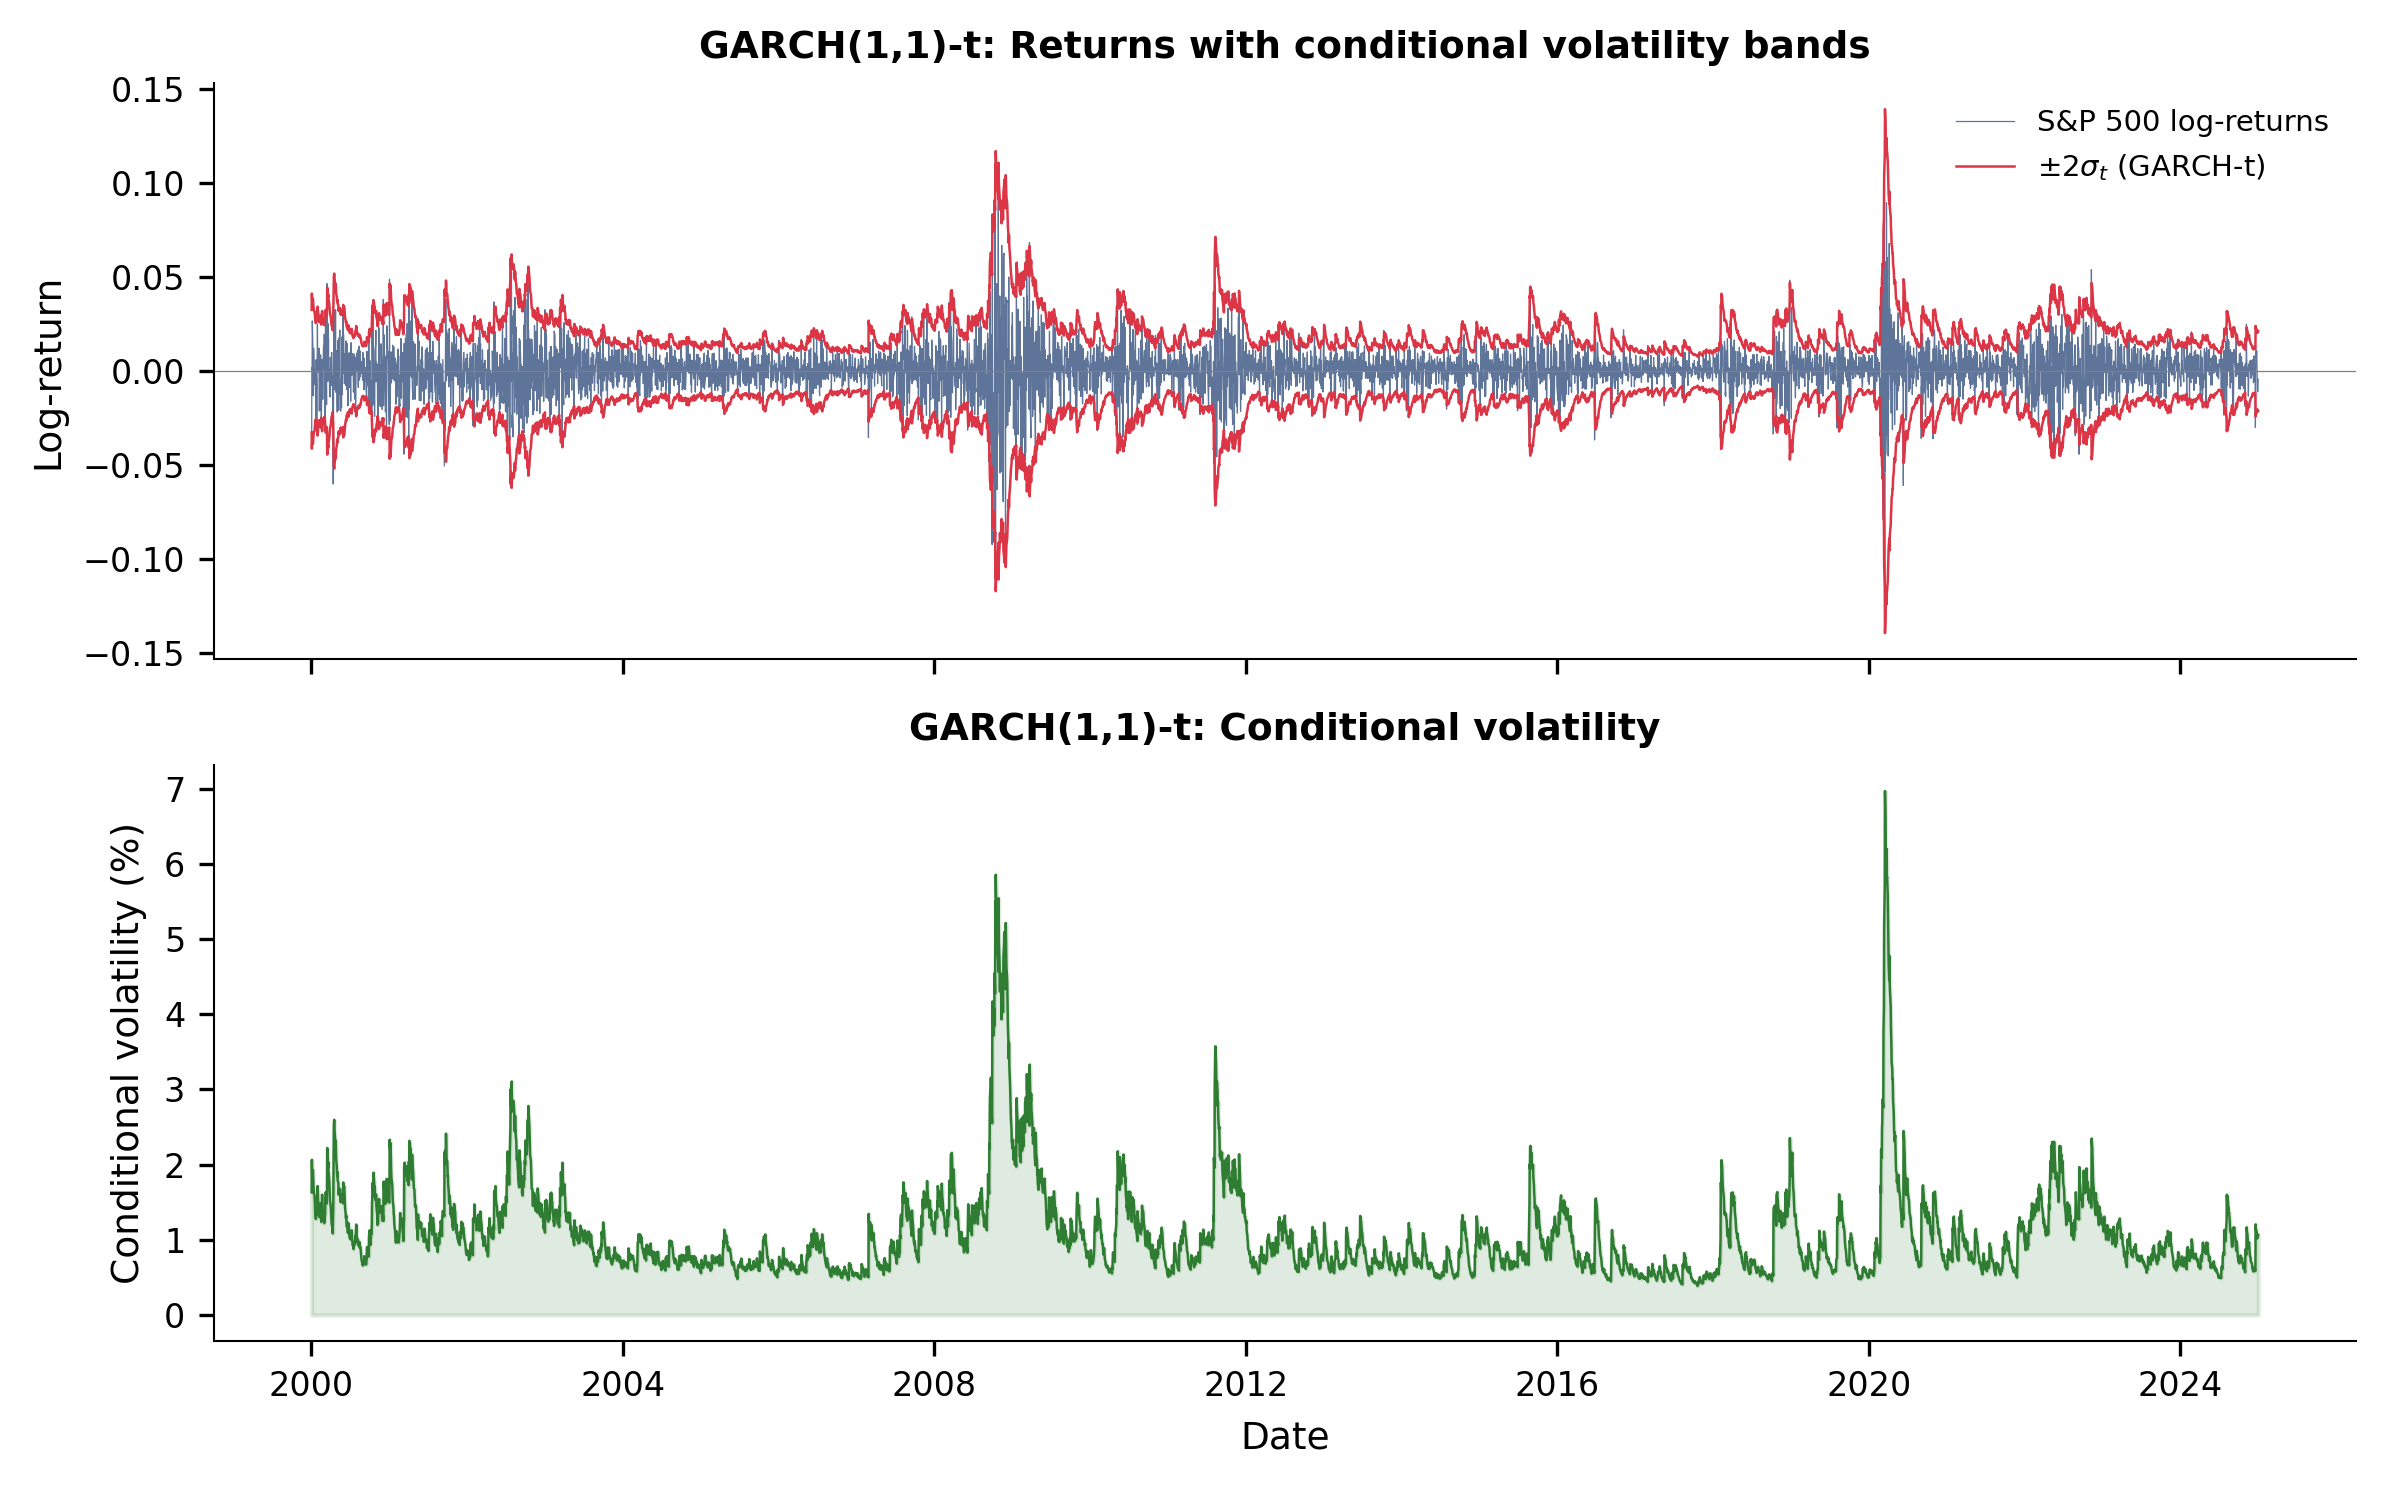
\includegraphics[width=0.38\textwidth]{ch2_garch_t_fit.png}
\end{center}
\quantlet{SFM\_ch2\_garch\_t}{https://github.com/QuantLet/Stat_fin_markets/tree/master/Ch_02/SFM_ch2_modern_extensions}
\end{frame}

%--- MSc Slide 3 ---
\slidelevel{MSc}
\begin{frame}{Mixturi Gaussiene și schimbarea de regim}
\vspace{-0.15cm}
\begin{columns}[T]
\begin{column}{0.55\textwidth}
\begin{block}{Mixturi Gaussiene}
\vspace{-0.3cm}
\[
f(x) = \sum_{k=1}^K \pi_k\,\phi(x;\mu_k, \sigma_k^2)
\]
\vspace{-0.3cm}
\begin{itemize}
\item $K=2$: regim calm ($\sigma_1$ mic) + criză ($\sigma_2$ mare); EM
\end{itemize}
\end{block}
\begin{block}{Schimbarea de regim Hamilton (1989)}
\begin{itemize}
\item Lanț Markov latent $s_t \in \{1,2\}$; \quad $r_t \mid s_t \sim N(\mu_{s_t}, \sigma_{s_t}^2)$
\item Probabilitățile de tranziție estimate prin MLE
\end{itemize}
\end{block}
\end{column}
\begin{column}{0.43\textwidth}
\begin{center}
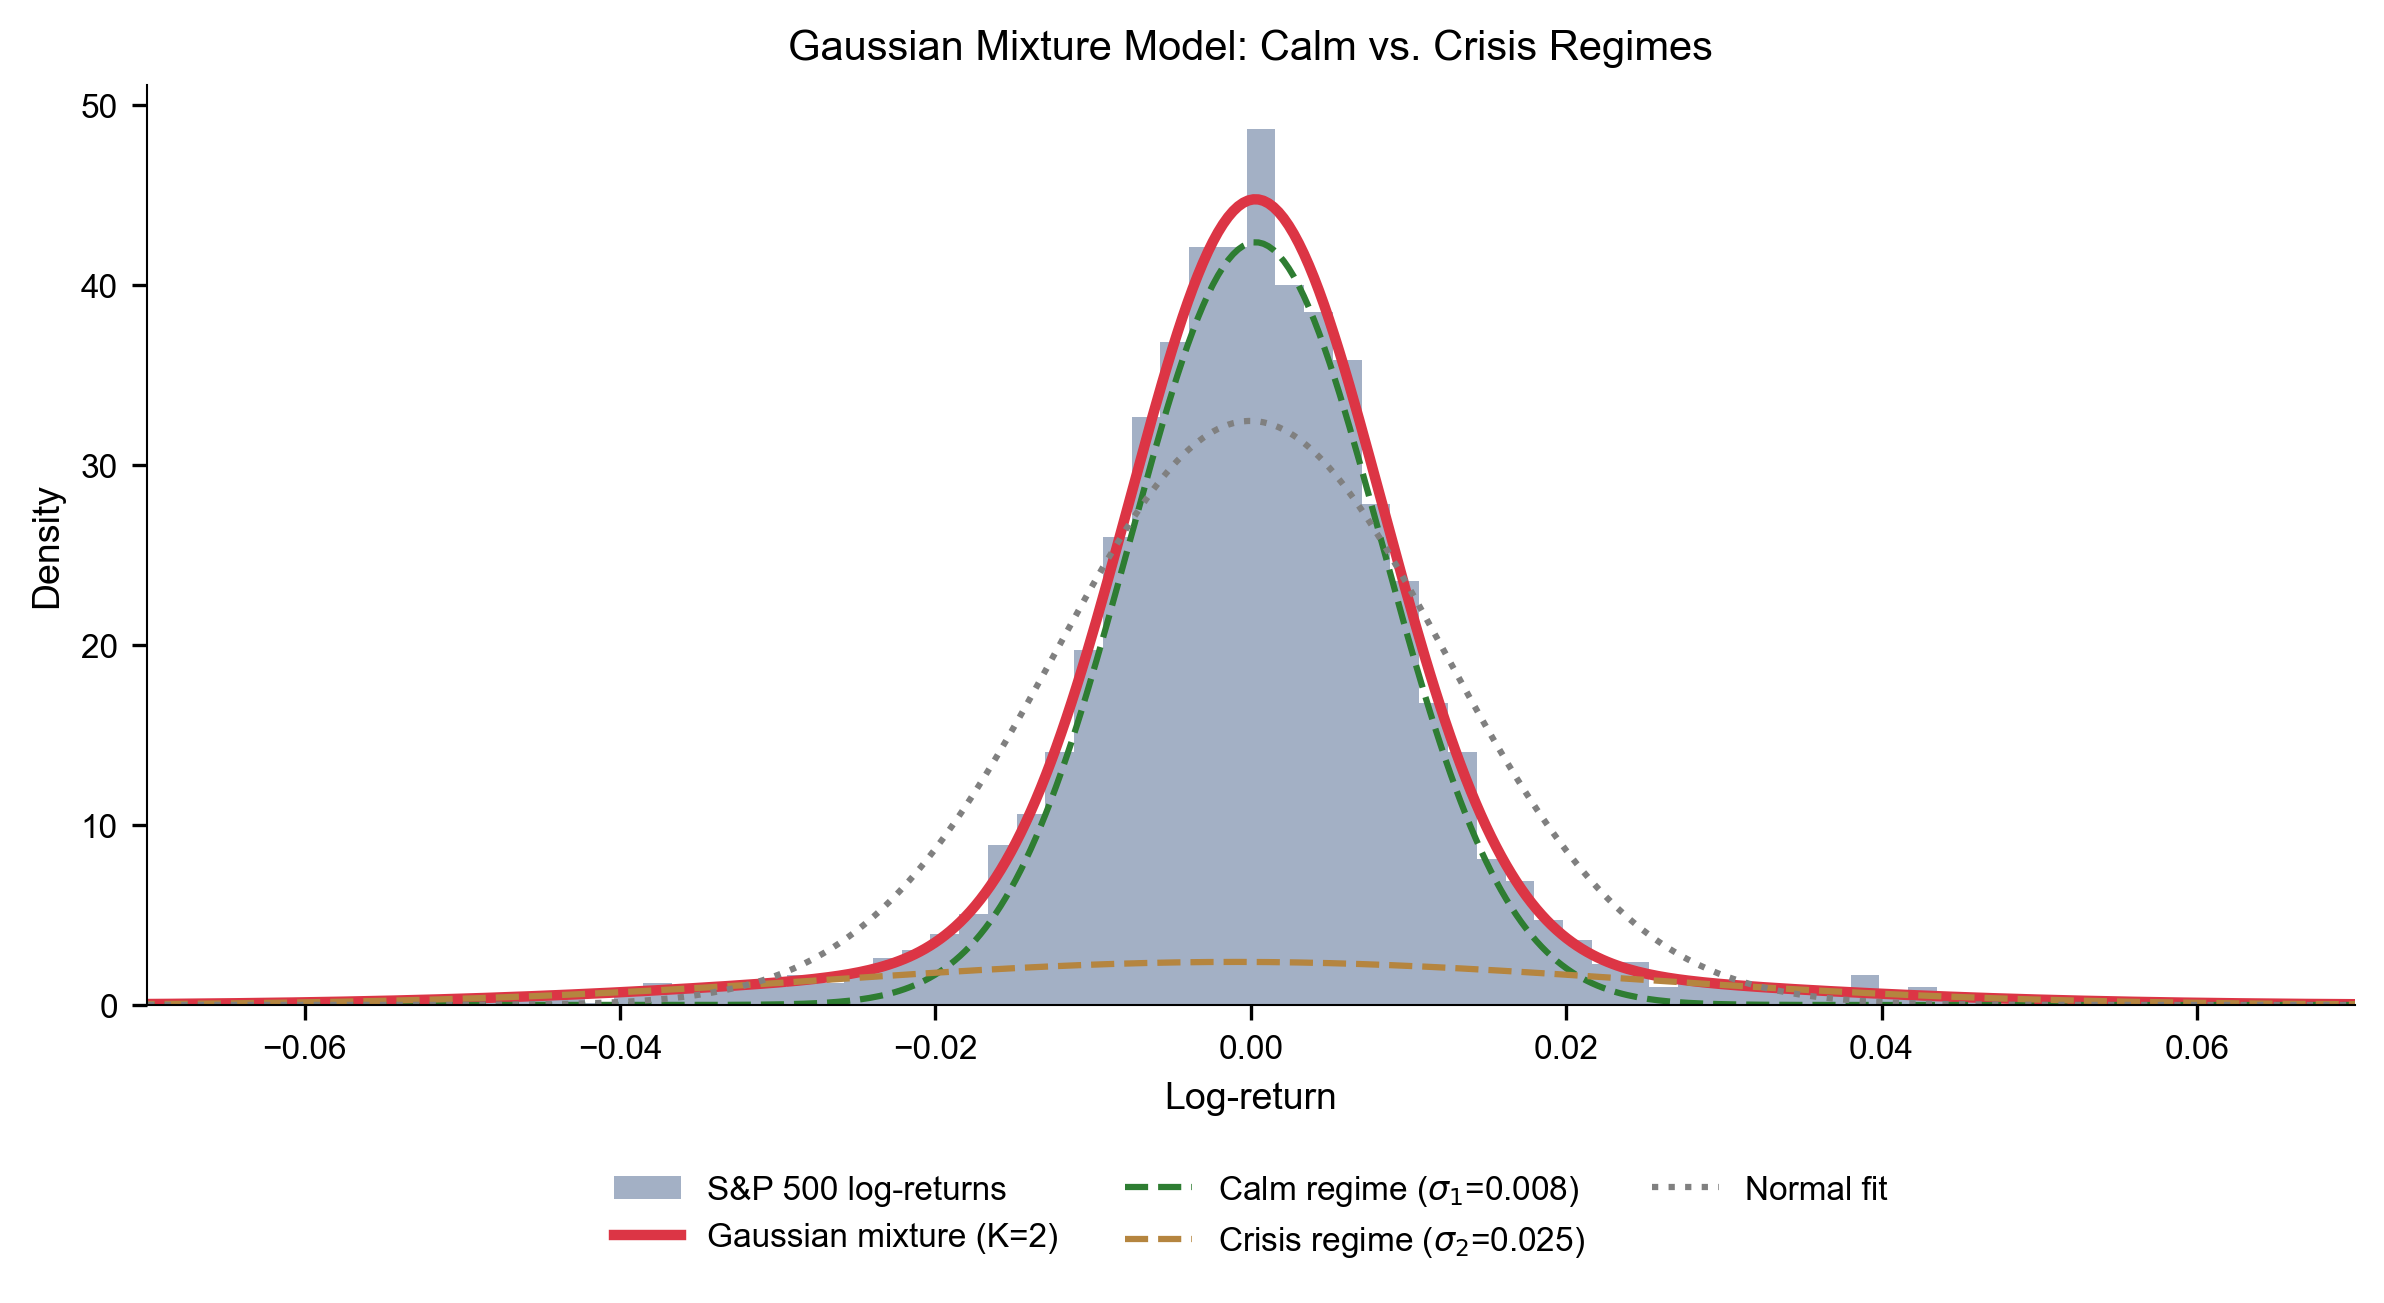
\includegraphics[width=0.85\textwidth]{ch2_gaussian_mixture.png}
\end{center}
\quantlet{SFM\_ch2\_mixture}{https://github.com/QuantLet/Stat_fin_markets/tree/master/Ch_02/SFM_ch2_modern_extensions}
\end{column}
\end{columns}
\end{frame}

%--- MSc Slide 4 ---
\slidelevel{MSc}
\begin{frame}{Clasificarea regimurilor}
\begin{center}
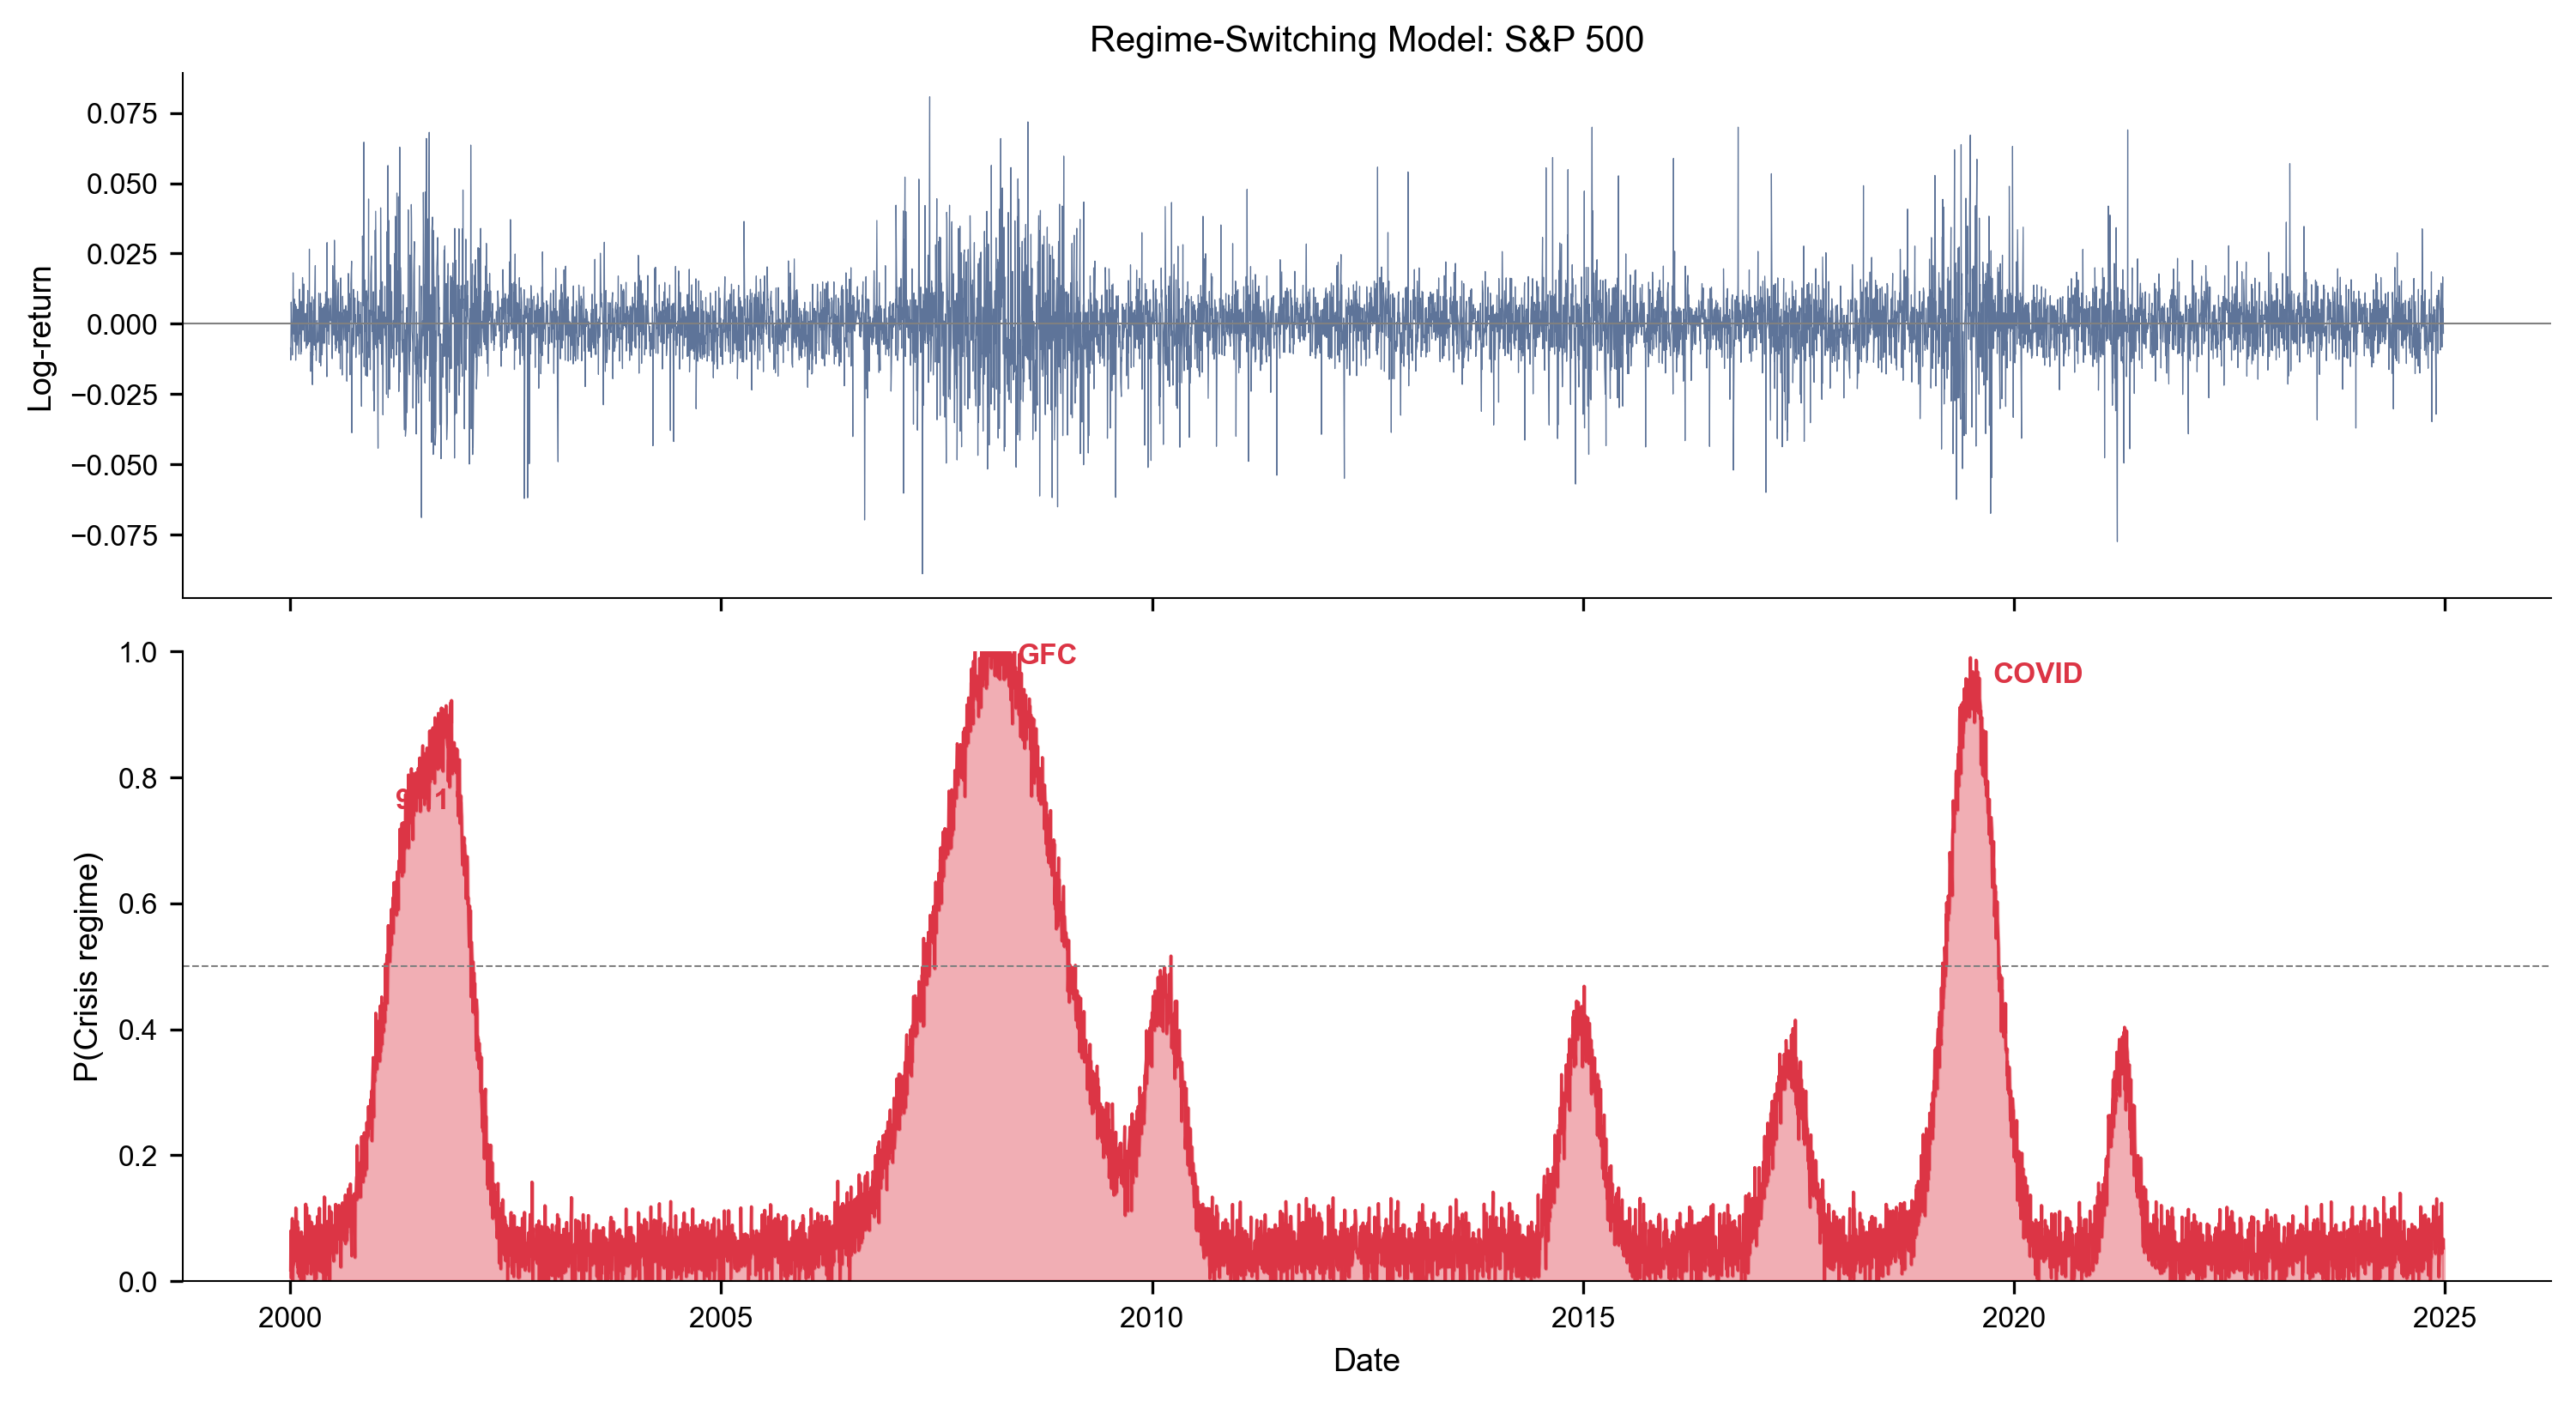
\includegraphics[width=0.55\textwidth]{ch2_regime_classification.png}
\end{center}
\vspace{-0.2cm}
\quantlet{SFM\_ch2\_modern\_extensions}{https://github.com/QuantLet/Stat_fin_markets/tree/master/Ch_02/SFM_ch2_modern_extensions}
\vspace{-0.1cm}
\begin{itemize}
\item Probabilitatea netedă de a fi în regimul de ,,criză'' (2001, 2008--2009, 2020)
\item Schimbarea de regim surprinde riscul de coadă variabil în timp
\end{itemize}
\end{frame}

%--- PhD Slide 5 ---
\slidelevel{PhD}
\begin{frame}{Volatilitate stochastică și difuzii cu salturi}
\begin{itemize}
\item \textbf{Volatilitate stochastică}:
\[
d\ln\sigma_t^2 = \kappa(\theta - \ln\sigma_t^2)\,dt + \sigma_v\,dW_t^v
\]
cu $\Corr(dW_t, dW_t^v) = \rho$ (levier)
\item \textbf{Difuzie cu salturi} (Merton, 1976):
\[
dS/S = \mu\,dt + \sigma\,dW + J\,dN_t
\]
unde $N_t$ este un proces Poisson, $J \sim N(\mu_J, \sigma_J^2)$
\item Kou (2002): salturi dublu-exponențiale pentru tratabilitate analitică
\item Aceste modele generează simultan cozi groase și clusterizarea volatilității
\end{itemize}
\end{frame}

%--- PhD Slide 6 ---
\slidelevel{PhD}
\begin{frame}{Modele conduse de procese L\'{e}vy}
\begin{itemize}
\item \textbf{Modelul BNS} (Barndorff-Nielsen \& Shephard, 2001):
\[
dX_t = (\mu + \beta\sigma_t^2)\,dt + \sigma_t\,dW_t, \quad d\sigma_t^2 = -\lambda\sigma_t^2\,dt + dL_{\lambda t}
\]
unde $L_t$ este un subordonator (proces L\'{e}vy crescător)
\item \textbf{GARCH cu inovații stabile}: Mittnik \& Rachev (1993)
\item \textbf{Volatilitate realizată}: $RV_t = \sum_{i=1}^{M} r_{t,i}^2$ (frecvență înaltă)
\item GARCH integrat fracționar (FIGARCH) pentru memoria lungă în volatilitate
\end{itemize}
\end{frame}

%--- PhD Slide 7 ---
\slidelevel{PhD}
\begin{frame}{Măsuri realizate și microstructură}
\begin{itemize}
\item \textbf{Varianța realizată}: $RV_t = \sum_{i=1}^M r_{t,i}^2 \xrightarrow{p} \int_0^1 \sigma_s^2\,ds$ când $M \to \infty$
\item \textbf{Zgomot de microstructură}: la frecvențe foarte înalte, săritura bid-ask distorsionează $RV$
\item \textbf{Corecții}: subeșantionare, estimatori kernel (Barndorff-Nielsen et al., 2008)
\item \textbf{Detectarea salturilor}: variația bipower separă componentele continuă și de salt
\item Distribuția randamentelor \textit{condiționată de} volatilitatea realizată este mai aproape de Gaussiană (deformarea timpului)
\end{itemize}
\end{frame}

%--- Y3 Slide 8 ---
\slidelevel{Y3}
\begin{frame}{Exemplu GARCH(1,1) --- Calcul pas cu pas}
\begin{exampleblock}{Exercițiu}
Un model GARCH(1,1) estimat pe randamentele zilnice S\&P~500 dă:
$\omega = 0{,}00001$, $\alpha = 0{,}09$, $\beta = 0{,}90$. Calculați varianța necondiționată, persistența și timpul de înjumătățire.
\end{exampleblock}

\begin{block}{Rezolvare}
\begin{enumerate}
\item \textbf{Persistență}: $\alpha + \beta = 0{,}99 < 1$ \checkmark\ (staționaritate)
\item \textbf{Varianța necondiționată}: $\bar{\sigma}^2 = \frac{\omega}{1 - \alpha - \beta} = \frac{0{,}00001}{0{,}01} = 0{,}001 \;\Rightarrow\; \bar{\sigma} = 3{,}16\%$
\item \textbf{Half-life}: $h = \frac{\ln 2}{\ln(1/0{,}99)} = \frac{0{,}693}{0{,}01005} \approx 69$ zile ($\approx 3$ luni)
\end{enumerate}
\end{block}

\begin{rmk}
\begin{itemize}
\item Un șoc de volatilitate se reduce la jumătate abia după $\approx 69$ zile de tranzacționare
\end{itemize}
\end{rmk}
\end{frame}

%=============================================================================
% SECȚIUNEA 12: STUDIU DE CAZ
%=============================================================================
\section{Studiu de caz}

%--- Y3 Slide 0: Distribuții și metode utilizate în studiul de caz ---
\slidelevel{Y3}
\begin{frame}{Studiu de caz: Distribuțiile candidate}
    \begin{block}{Cele 6 distribuții testate (rezumat din Cap.\ 2a--2b)}
    \small
    \begin{enumerate}
        \item \textbf{Normală} ($k\!=\!2$): $f(x) = \frac{1}{\sigma\sqrt{2\pi}}\exp\!\bigl(-\frac{(x-\mu)^2}{2\sigma^2}\bigr)$ --- cozi exponențiale
        \item \textbf{Student-$t$} ($k\!=\!3$): cozi $\sim |x|^{-(\nu+1)}$; \; $\hat{\nu} \approx 3$--$5$ pentru acțiuni
        \item \textbf{Cauchy}: Student-$t$ cu $\nu = 1$ --- $\E[X]$ nedefinit, cozi foarte groase
        \item \textbf{Laplace} ($k\!=\!2$): GED cu $\nu = 1$, i.e.\ $f(x) \propto \exp(-|x|/b)$ --- exponențială dublă
        \item \textbf{GED} ($k\!=\!3$): $f(x;\nu) = \frac{\nu}{2\lambda\,\Gamma(1/\nu)}\exp\!\bigl(-\bigl|\frac{x}{\lambda}\bigr|^\nu\bigr)$; \; $\nu < 2$ $\Rightarrow$ cozi mai groase ca distribuția normală
        \item \textbf{Historical VaR}: VaR $=$ cuantila empirică a ferestrei de randamente --- neparametric, fără ipoteză distribuțională
    \end{enumerate}
    \end{block}

    \begin{rmk}
    \begin{itemize}
    \item Selecția se face prin $\text{AIC} = -2\ell + 2k$ și $\text{BIC} = -2\ell + k\ln n$ (cf.\ Secțiunea~8)
    \end{itemize}
    \end{rmk}
\end{frame}

%--- Y3 Slide 1: Selecția modelului ---
\slidelevel{Y3}
\begin{frame}{Studiu de caz: Selecția modelului}
\quantlet{SFM\_ch2\_case\_study\_2c}{https://github.com/QuantLet/Stat_fin_markets/tree/master/Ch_02/SFM_ch2_case_study_2c}
    \begin{columns}[T]
        \begin{column}{0.55\textwidth}
            \begin{block}{Heatmap AIC/BIC: 6 distribuții $\times$ 3 active}
            \small
            \begin{itemize}
                \item Culorile indică \textbf{$\Delta$AIC} relativ la cel mai bun model
                \item Chenarul verde = modelul optim per activ
                \item \textbf{Student-t} și \textbf{GED} domină pe S\&P 500 și BRD
                \item Pentru Bitcoin: GED câștigă ușor (cozi mai flexibile)
                \item Normal și Cauchy sunt consistent cele mai slabe
            \end{itemize}
            \end{block}
        \end{column}
        \begin{column}{0.42\textwidth}
            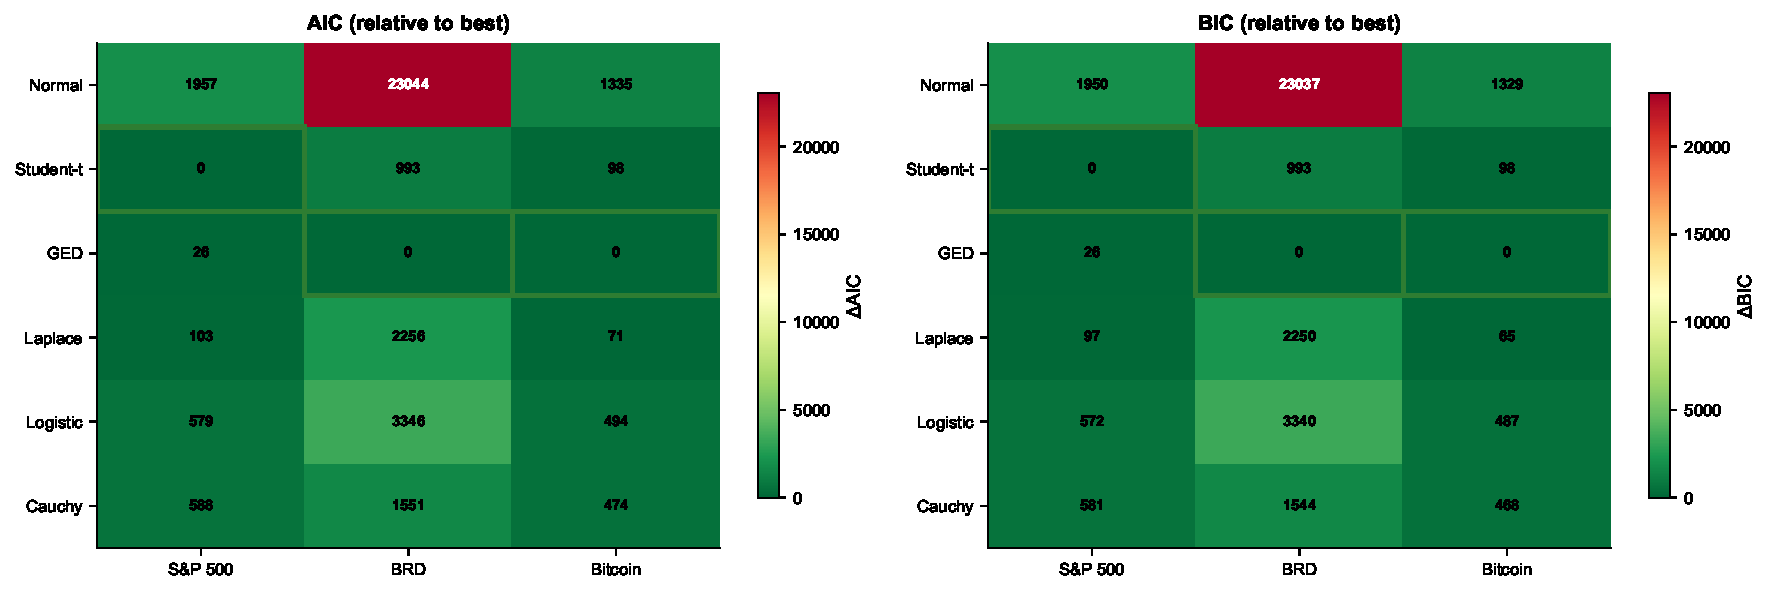
\includegraphics[width=\textwidth]{../../charts/ch2_cs2c_model_selection_heatmap.pdf}
        \end{column}
    \end{columns}
\end{frame}

%--- Y3 Slide 2: Dependența de coadă ---
\slidelevel{Y3}
\begin{frame}{Studiu de caz: Dependența de coadă}
\quantlet{SFM\_ch2\_case\_study\_2c}{https://github.com/QuantLet/Stat_fin_markets/tree/master/Ch_02/SFM_ch2_case_study_2c}
    \begin{columns}[T]
        \begin{column}{0.55\textwidth}
            \begin{block}{Copula empirică: S\&P 500 vs BRD}
            \small
            Transformare rang $\to$ uniform $[0,1]$:
            \begin{itemize}
                \item \textbf{Panoul stâng}: copula completă — dependență vizibilă
                \item \textbf{Centru}: zoom coada inferioară ($< 10\%$) — $\hat{\lambda}_L > 0$
                \item \textbf{Dreapta}: zoom coada superioară ($> 90\%$) — $\hat{\lambda}_U$ mai mic
                \item \textbf{Asimetrie}: cozile stângi mai dependente decât cele drepte
            \end{itemize}
            \vspace{0.1cm}
            $\Rightarrow$ \emph{Diversificarea scade exact când avem nevoie de ea!}
            \end{block}
        \end{column}
        \begin{column}{0.42\textwidth}
            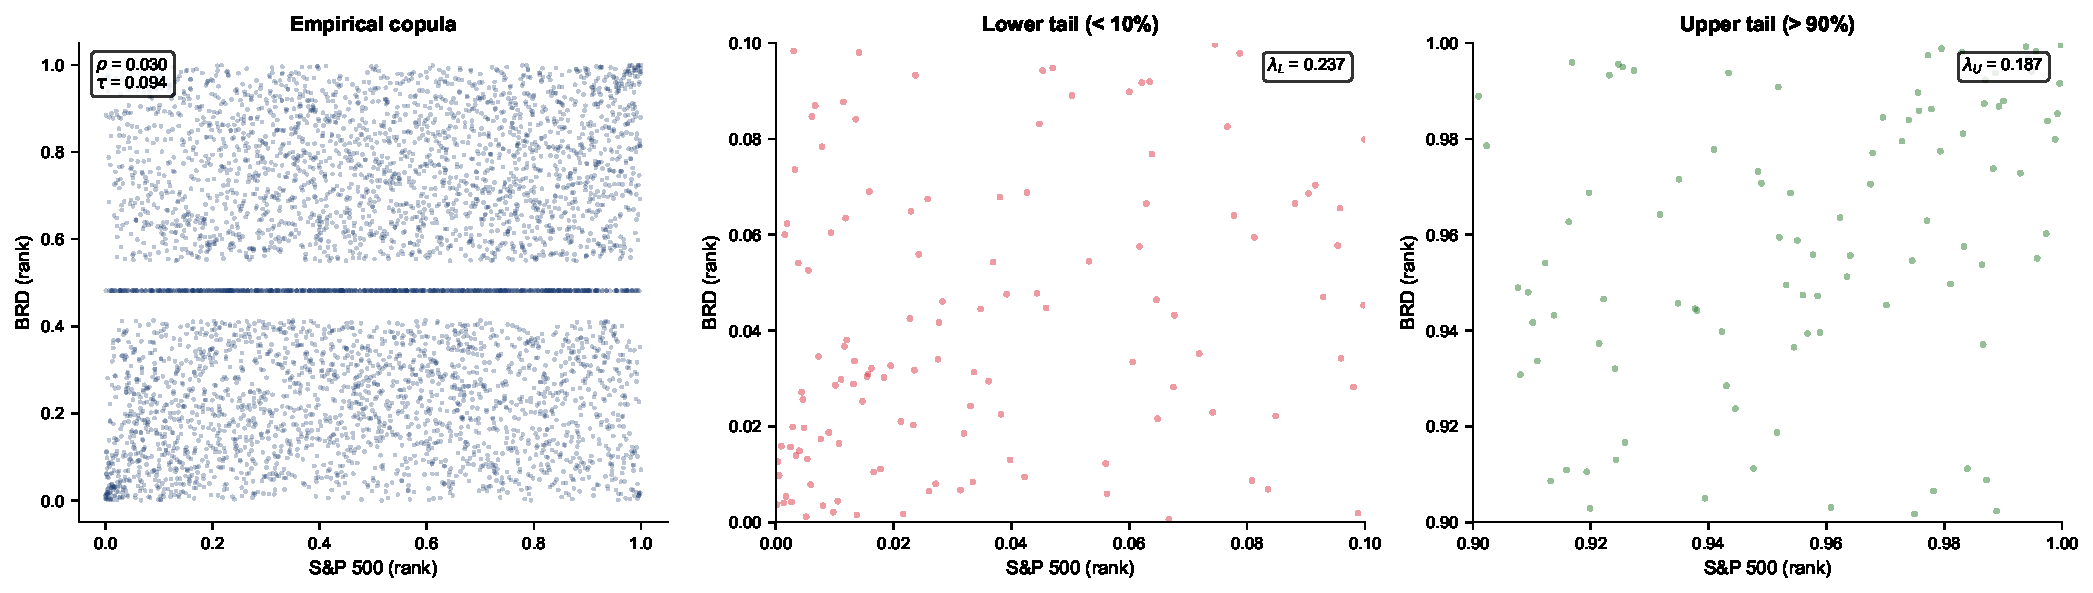
\includegraphics[width=\textwidth]{../../charts/ch2_cs2c_copula_scatter.pdf}
        \end{column}
    \end{columns}
\end{frame}

%--- Y3 Slide 3: VaR/ES complet ---
\slidelevel{Y3}
\begin{frame}{Studiu de caz: VaR/ES pe toate modelele}
    \begin{center}
        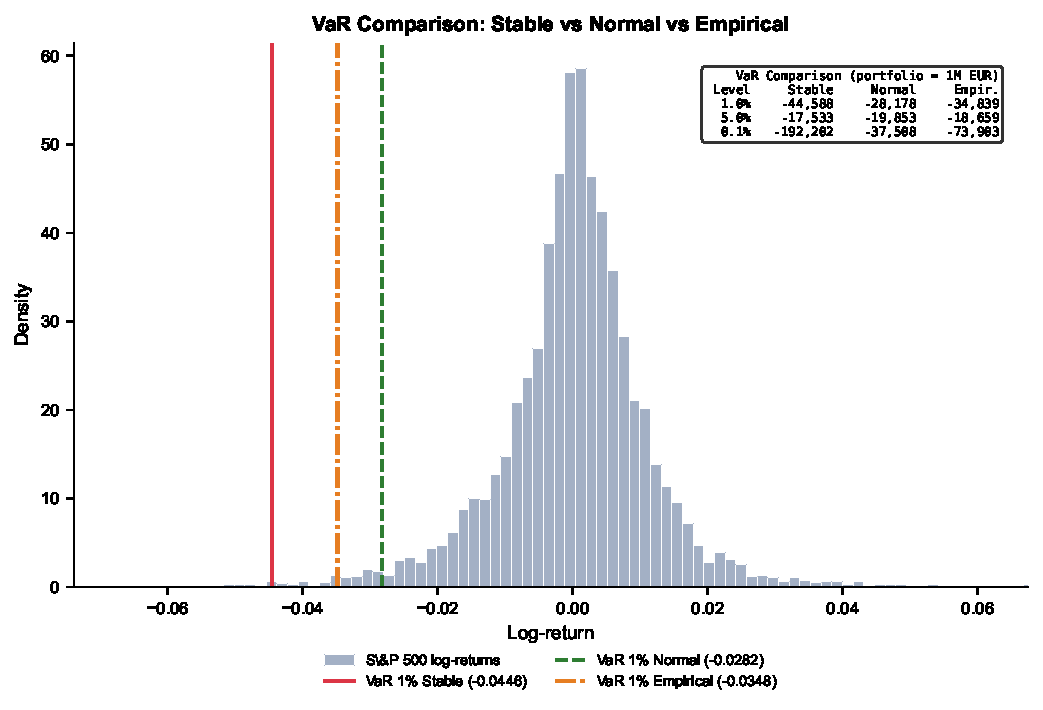
\includegraphics[width=0.58\textwidth]{../../charts/ch2_var_comparison.pdf}
    \end{center}
    \vspace{-0.4cm}
    {\footnotesize VaR/ES 1\% pe 6 distribuții $\times$ 3 active. Cauchy supraestimează; Student-t, GED: interval rezonabil. ES diferențiază mai bine (coerență).}
\end{frame}

%--- Y3 Slide 4: Backtest pe crize ---
\slidelevel{Y3}
\begin{frame}{Studiu de caz: Backtest VaR pe crize}
\quantlet{SFM\_ch2\_case\_study\_2c}{https://github.com/QuantLet/Stat_fin_markets/tree/master/Ch_02/SFM_ch2_case_study_2c}
    \begin{columns}[T]
        \begin{column}{0.55\textwidth}
            \begin{block}{Rolling VaR 1\%: GFC 2008 și COVID 2020}
            \small
            Fereastră rulantă de 250 zile:
            \begin{itemize}
                \item \textcolor{MainBlue}{Normal VaR} ($= 2{,}326\,\hat{\sigma}$): cele mai multe depășiri
                \item \textcolor{IDAred}{Student-t VaR}: mai puține depășiri
                \item \textcolor{Forest}{Historical VaR} (cuantila empirică a ferestrei): se adaptează cu întârziere
            \end{itemize}
            \vspace{0.1cm}
            \footnotesize Test Kupiec: $LR_{uc} = -2\ln\frac{\alpha^x(1-\alpha)^{n-x}}{\hat{p}^x(1-\hat{p})^{n-x}}$; \; $\hat{p} = x/n$
            \end{block}
        \end{column}
        \begin{column}{0.42\textwidth}
            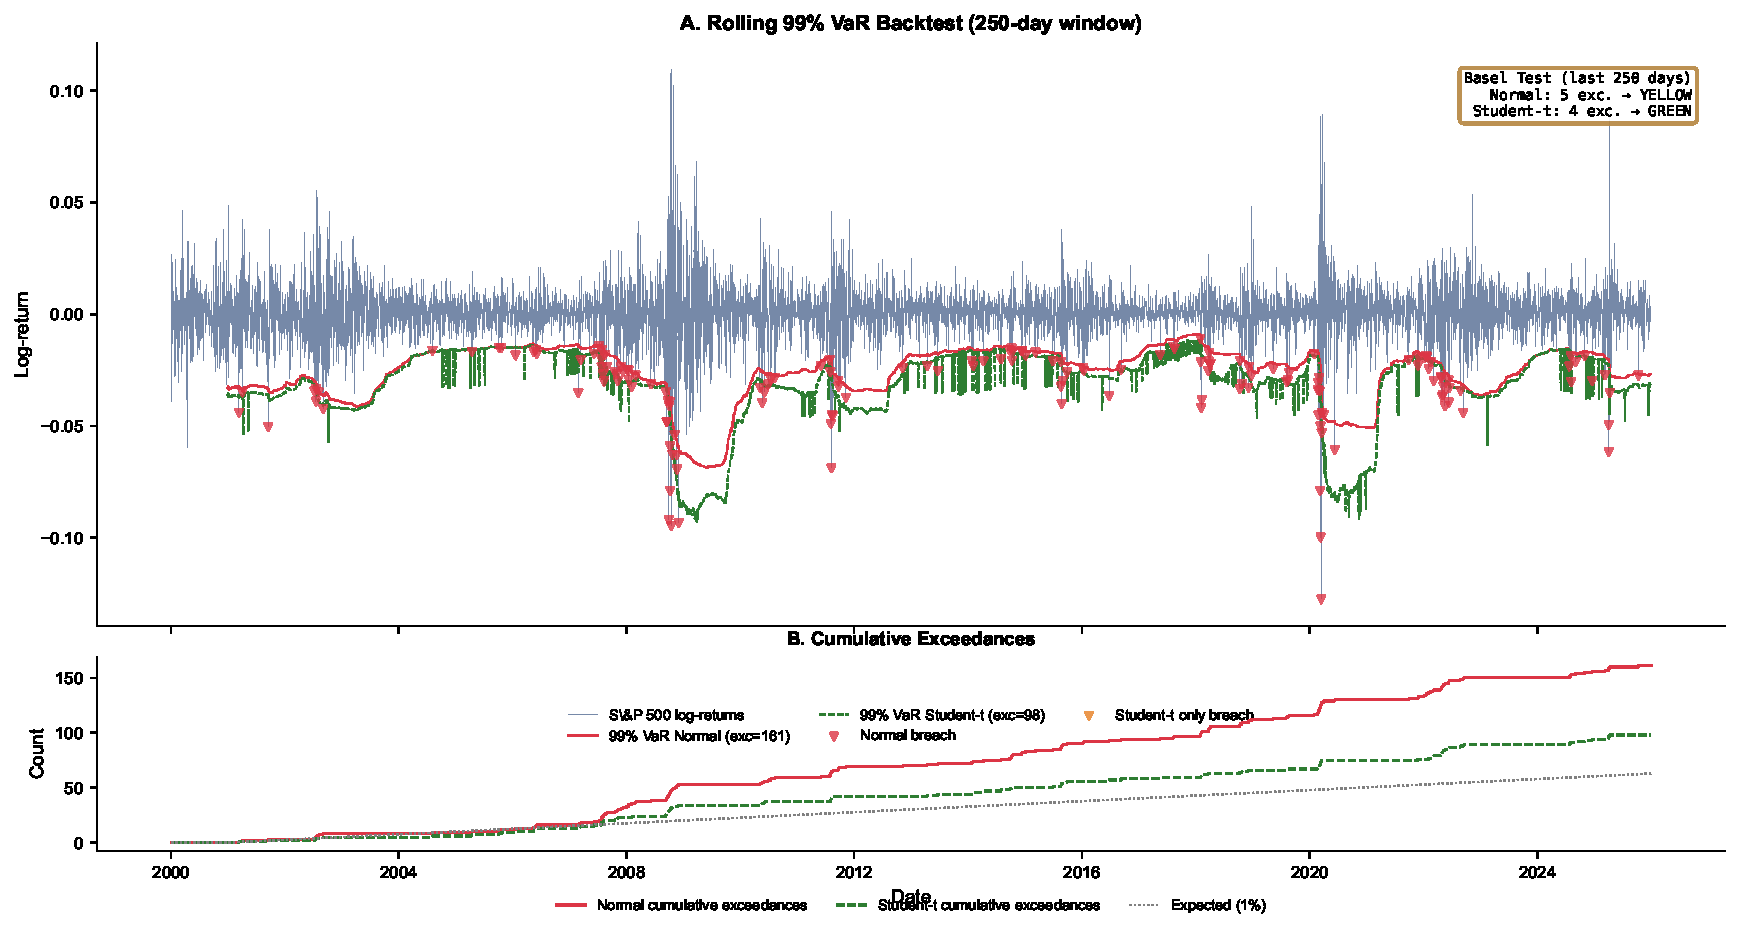
\includegraphics[width=\textwidth]{../../charts/ch2_var_backtest.pdf}
        \end{column}
    \end{columns}
\end{frame}

%--- Y3 Slide 5: Semaforul Basel ---
\slidelevel{Y3}
\begin{frame}{Studiu de caz: Semaforul Basel}
    \begin{columns}[T]
        \begin{column}{0.55\textwidth}
            \begin{block}{Traffic Light Test (250 zile, VaR 1\%)}
            \small
            Clasificarea Basel:
            \begin{itemize}
                \item \textcolor{Forest}{\textbf{Verde}}: 0--4 exceedances (model acceptat)
                \item \textcolor{Amber}{\textbf{Galben}}: 5--9 exceedances (penalizare capital)
                \item \textcolor{IDAred}{\textbf{Roșu}}: $\geq 10$ exceedances (model respins)
            \end{itemize}
            \vspace{0.1cm}
            Numerele din cercuri = exceedances observate.
            \end{block}
        \end{column}
        \begin{column}{0.42\textwidth}
            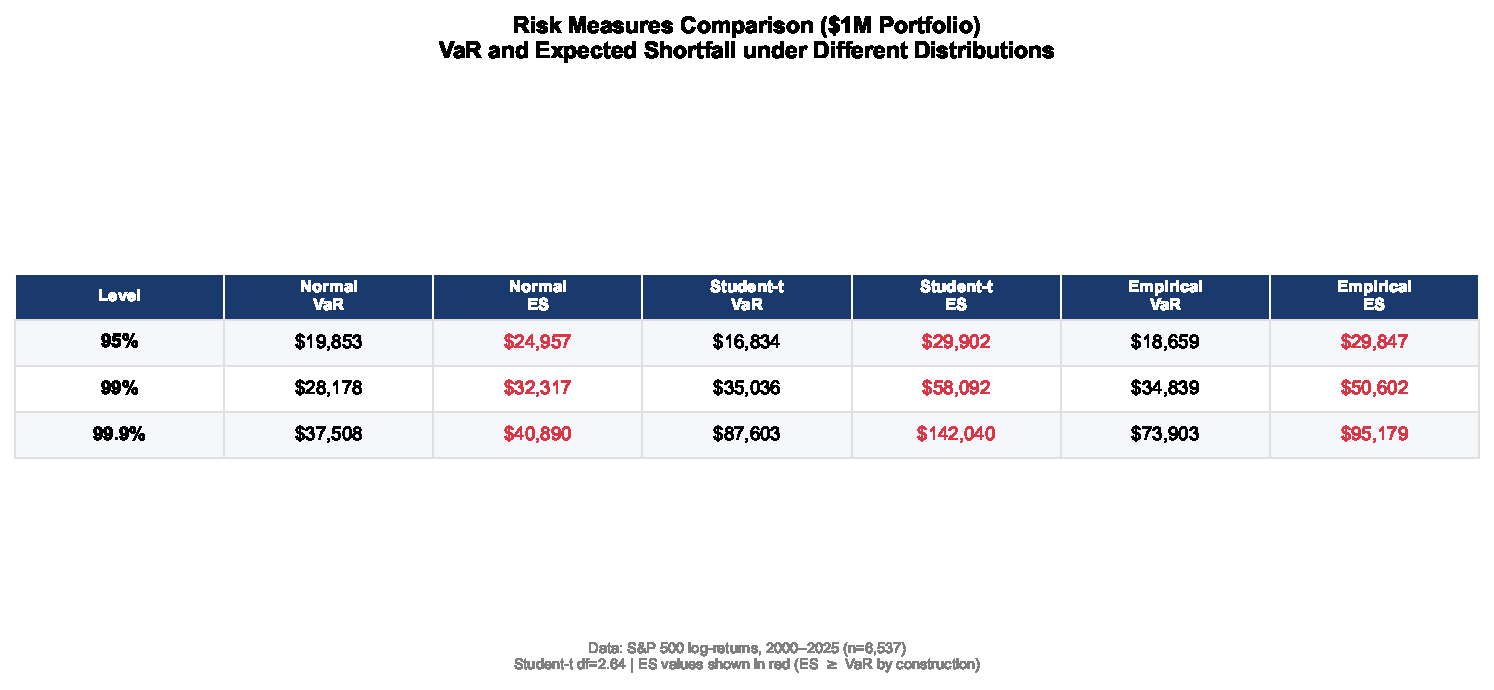
\includegraphics[width=\textwidth]{../../charts/ch2_risk_comparison_table.pdf}
        \end{column}
    \end{columns}

    \vspace{-0.2cm}
    {\footnotesize Kupiec: Normal respins ($\hat{p} \gg 1\%$, $LR_{uc}$: $p < 0{,}001$); Student-$t$ acceptat ($\hat{p} \approx 1\%$).}
\end{frame}

%--- Y3 Slide 6: Lecția finală ---
\slidelevel{Y3}
\begin{frame}{Studiu de caz: Lecția finală}
    \begin{block}{Pipeline complet de măsurare a riscului}
    \small
    \begin{enumerate}\setlength{\itemsep}{0pt}
        \item \textbf{Datele}: descarcă, curăță, calculează log-randamente
        \item \textbf{Diagnostic}: kurtosis, QQ-plot, teste de normalitate
        \item \textbf{Estimare index coadă}: Hill plot, $\hat{\alpha}_{\text{Hill}}$
        \item \textbf{Selectează distribuția}: AIC/BIC pe set de candidați
        \item \textbf{Calculează VaR/ES}: la cuantilele relevante (1\%, 2.5\%)
        \item \textbf{Validează}: backtest + semaforul Basel
    \end{enumerate}
    \end{block}
    \vspace{-0.2cm}
    \begin{alertblock}{Reguli practice}
    \small
        \begin{itemize}\setlength{\itemsep}{0pt}
            \item Nu folosi niciodată \emph{doar} modelul Normal pentru managementul riscului
            \item Întotdeauna fă backtest \emph{înainte} de a lua o decizie
            \item Diversificarea \textbf{scade} în perioade de criză — ia în calcul dependența de coadă
        \end{itemize}
    \end{alertblock}
\end{frame}

%=============================================================================
% SECȚIUNEA 13: REZUMAT
%=============================================================================
\section{Rezumat}

%--- Y3 Slide 1 ---
\slidelevel{Y3}
\begin{frame}{Concluzii cheie}
    \begin{block}{Rezumat}
    \small
    \begin{itemize}
        \item \textbf{Randamentele financiare nu sunt normale}: cozi groase (\textit{heavy tails}), asimetrie, clusterizarea volatilității
        \item \textbf{Student-$t$}: cel mai simplu model cu cozi groase, surprinde excesul de kurtosis (\textit{excess kurtosis})
        \item \textbf{Distribuții stabile}: motivate teoretic (TLCG), varianță infinită posibilă
        \item \textbf{EVT}: cadru riguros pentru modelarea cozilor extreme
        \item \textbf{VaR și ES}: alegerea distribuției afectează direct măsurarea riscului
        \begin{itemize}
            \item VaR 1\% sub Normală $\ll$ VaR 1\% sub Student-$t$ $\ll$ VaR 1\% sub Stabilă
        \end{itemize}
        \item \textbf{Nu există un singur model cel mai bun}: alegerea depinde de aplicație
    \end{itemize}
    \end{block}
\end{frame}

%--- Y3 Slide 2 ---
\slidelevel{Y3}
\begin{frame}{Formule importante}
    \begin{columns}[T]
        \begin{column}{0.48\textwidth}
        {\small
        \begin{block}{Distribuții cheie}
            \begin{itemize}
                \item \textbf{Normală}: $f(x) = \frac{1}{\sigma\sqrt{2\pi}}e^{-\frac{(x-\mu)^2}{2\sigma^2}}$
                \item \textbf{Student-$t$}: $\kappa_e = 6/(\nu-4)$ pentru $\nu > 4$
                \item \textbf{Stabilă}: $\varphi(t) = \exp\{i\delta t - \gamma|t|^\alpha[1+i\beta\mathrm{sgn}(t)\omega]\}$
            \end{itemize}
        \end{block}
        \begin{alertblock}{Măsuri de risc}
            \begin{itemize}
                \item \textbf{VaR}: $P(X \leq -\text{VaR}_\alpha) = \alpha$
                \item \textbf{ES}: $\E[-X \mid X \leq -\text{VaR}_\alpha]$
                \item \textbf{GPD}: $G_{\xi,\sigma}(y) = 1 - (1+\xi y/\sigma)^{-1/\xi}$
            \end{itemize}
        \end{alertblock}
        }
        \end{column}
        \begin{column}{0.48\textwidth}
        {\small
        \begin{exampleblock}{Criterii de selecție}
            \begin{itemize}
                \item \textbf{AIC}: $-2\ell + 2k$
                \item \textbf{BIC}: $-2\ell + k\ln n$
                \item \textbf{QQ}: grafic cuantilă-cuantilă
            \end{itemize}
        \end{exampleblock}
        \begin{block}{Fapte stilizate}
            \begin{itemize}
                \item Exces de kurtosis $> 0$
                \item Asimetrie negativă
                \item Clusterizarea volatilității
                \item $|r_t|$ autocorelat
            \end{itemize}
        \end{block}
        }
        \end{column}
    \end{columns}
\end{frame}

%--- Y3 Slide 2 ---
\slidelevel{Y3}
\begin{frame}{Teme pentru acasă}
\begin{block}{Anul 3}
\begin{enumerate}
\item Descărcați 5 ani de prețuri zilnice pentru o acțiune. Calculați log-randamentele, momentele eșantionului și testați normalitatea (Jarque--Bera).
\item Ajustați distribuțiile normală și Student-$t$ prin MLE. Comparați prin AIC/BIC și grafice QQ.
\item Calculați VaR 1\% și VaR 0{,}1\% sub ambele modele pentru un portofoliu de \$1M.
\end{enumerate}
\end{block}
\begin{block}{Master}
\begin{enumerate}\setcounter{enumi}{3}
\item Ajustați Student-$t$ asimetrică Hansen și calculați ES la nivelul de 1\%.
\item Efectuați un backtest VaR cu fereastră mobilă (250 zile) și aplicați testul Kupiec.
\end{enumerate}
\end{block}
\end{frame}

%--- MSc Slide 3 ---
\slidelevel{MSc}
\begin{frame}{Teme avansate}
\begin{enumerate}\setcounter{enumi}{5}
\item Ajustați o distribuție stabilă pe datele voastre folosind MLE. Raportați $(\hat{\alpha}, \hat{\beta}, \hat{\gamma}, \hat{\delta})$.
\item Aplicați metoda POT: selectați pragul, ajustați GPD, calculați VaR 1\% și ES bazate pe EVT.
\item Comparați toate modelele (normală, Student-$t$, Student-$t$ asim., stabilă, EVT) într-un tabel rezumativ.
\end{enumerate}

\vspace{0.3cm}
\textbf{Master}:
\begin{enumerate}\setcounter{enumi}{8}
\item Implementați estimatorul Hill. Creați un grafic Hill (\textit{Hill plot}) și discutați compromisul bias-varianță.
\item Ajustați un model GARCH(1,1)-$t$. Comparați distribuția reziduurilor standardizate (\textit{standardized residuals}) cu distribuția necondiționată a randamentelor.
\end{enumerate}
\end{frame}

%--- PhD Slide 4 ---
\slidelevel{PhD}
\begin{frame}{Direcții de cercetare}
\begin{itemize}
\item \textbf{Întrebări deschise}:
\begin{itemize}
\item Indicele real de coadă al randamentelor financiare este mai aproape de $\alpha \approx 3$ (varianță finită) sau $\alpha \approx 1{,}7$ (varianță infinită)?
\item Cum ar trebui să agregăm riscul când distribuțiile au varianță infinită?
\item Poate învățarea automată să îmbunătățească previziunea distribuțională?
\end{itemize}
\item \textbf{Lecturi recomandate}:
\begin{itemize}
\item Cont (2001): ,,Empirical properties of asset returns: stylized facts and statistical issues''
\item McNeil, Frey \& Embrechts (2015): \textit{Quantitative Risk Management}
\item Nolan (2020): \textit{Stable Distributions --- Models for Heavy Tailed Data}
\item Rachev (2003): \textit{Handbook of Heavy Tailed Distributions in Finance}
\end{itemize}
\end{itemize}
\end{frame}

%=============================================================================
% SECȚIUNEA: QUIZ
%=============================================================================

%=============================================================================
% SECTIUNEA: QUIZ
%=============================================================================
\section{Quiz}
\slidelevel{Y3}
\begin{frame}{Întrebarea 4}
    \begin{cminipage}{0.95\textwidth}
    \begin{alertblock}{Întrebare}
        \begin{itemize}
            \item Un portofoliu de \$10M are VaR zilnic la 1\% de: \$230k (normală), \$380k (Student-$t$, $\nu=5$), \$520k (stabilă, $\alpha=1{,}7$). Ce concluzie trageți?
        \end{itemize}
    \end{alertblock}

    \vspace{0.3cm}

    \begin{block}{Variante de răspuns}

        \textcolor{MainBlue}{\textbf{(A)}} Distribuția normală este cea mai conservatoare\\[3pt]

        \textcolor{MainBlue}{\textbf{(B)}} Alegerea distribuției nu afectează semnificativ VaR\\[3pt]

        \textcolor{MainBlue}{\textbf{(C)}} Subestimarea riscului de coadă sub ipoteza normală poate fi de $2\times$ sau mai mult\\[3pt]

        \textcolor{MainBlue}{\textbf{(D)}} Distribuția stabilă subestimează întotdeauna riscul

    \end{block}
    \end{cminipage}
\end{frame}

\slidelevel{Y3}
\begin{frame}{Întrebarea 4: Răspuns}
    \begin{cminipage}{0.95\textwidth}
    \begin{exampleblock}{Răspuns: (C)}
    \begin{itemize}
        \item VaR normală = \$230k, VaR stabilă = \$520k $\Rightarrow$ raportul este $520/230 \approx 2{,}3\times$.
        \item Distribuția normală \textbf{subestimează} riscul, nu este conservatoare (elimină A).
        \item Diferența de \$290k ($= 520 - 230$) este \textbf{foarte semnificativă} din perspectiva capitalului (elimină B).
        \item Aceasta demonstrează de ce Basel~III impune modele cu cozi groase.
    \end{itemize}
    \end{exampleblock}
    \end{cminipage}
\end{frame}

\slidelevel{Y3}
\begin{frame}{Întrebarea 6}
    \begin{cminipage}{0.95\textwidth}
    \begin{alertblock}{Întrebare}
        \begin{itemize}
            \item Modelul A are $\text{AIC} = 5200$ și modelul B are $\text{AIC} = 5180$ pe aceleași date. Ce concluzie este corectă?
        \end{itemize}
    \end{alertblock}

    \vspace{0.3cm}

    \begin{block}{Variante de răspuns}

        \textcolor{MainBlue}{\textbf{(A)}} Modelul A este mai bun (AIC mai mare)\\[3pt]

        \textcolor{MainBlue}{\textbf{(B)}} Modelul B este mai bun (AIC mai mic = mai bun)\\[3pt]

        \textcolor{MainBlue}{\textbf{(C)}} Nu putem compara fără BIC\\[3pt]

        \textcolor{MainBlue}{\textbf{(D)}} Diferența nu este semnificativă

    \end{block}
    \end{cminipage}
\end{frame}

\slidelevel{Y3}
\begin{frame}{Întrebarea 6: Răspuns}
    \begin{cminipage}{0.95\textwidth}
    \begin{exampleblock}{Răspuns: (B)}
    \begin{itemize}
        \item AIC = $-2\ell + 2k$: valori mai mici indică un echilibru mai bun între ajustare și complexitate.
        \item $\Delta\text{AIC} = 5200 - 5180 = 20 > 10$, ceea ce indică o preferință \textbf{puternică} pentru modelul B.
        \item (A) confundă direcția: AIC mai mic este mai bun.
        \item (C) este greșit: AIC singur este suficient pentru comparare, BIC oferă o perspectivă complementară.
    \end{itemize}
    \end{exampleblock}
    \end{cminipage}
\end{frame}

%=============================================================================
% SECTIUNEA: EXERCITII DE EXAMEN
%=============================================================================
\section{Exercitii de examen}
\slidelevel{MSc}
\begin{frame}{Exercițiul 6: Comparația distribuțiilor}
\begin{block}{Enunț}
Se dau rezultatele ajustării pe randamente S\&P~500 (10 ani, zilnice, $n = 2516$):
\begin{center}
{\small
\renewcommand{\arraystretch}{1.2}
\begin{tabular}{lcccc}
\toprule
Model & $k$ & $\ell$ & AIC & BIC \\
\midrule
Normal & 2 & 7890 & $-15{,}776$ & $-15{,}764$ \\
Student-$t$ & 3 & 8120 & $-16{,}234$ & $-16{,}216$ \\
Skew-$t$ & 4 & 8135 & $-16{,}262$ & $-16{,}239$ \\
Stabilă & 4 & 8095 & $-16{,}182$ & $-16{,}159$ \\
\bottomrule
\end{tabular}
}
\end{center}
\end{block}
\begin{enumerate}
    \item Verificați formulele AIC și BIC pentru modelul normal.
    \item Care model este preferat de AIC? Dar de BIC?
    \item De ce Skew-$t$ câștigă deși are mai mulți parametri?
    \item Stabilă are AIC mai slab decât Student-$t$. Înseamnă că este un model inferior? Discutați.
\end{enumerate}
\end{frame}

\slidelevel{MSc}
\begin{frame}{Exercițiul 7: VaR sub diferite distribuții}
\begin{block}{Enunț}
Un portofoliu de \$1M. Randamente zilnice cu $\hat{\mu} = 0{,}03\%$, $\hat{\sigma} = 1{,}5\%$.
\end{block}
\begin{enumerate}
    \item Calculați VaR 1\% sub ipoteza \textbf{normală}.
    \item Sub Student-$t$ ($\nu = 5$): $\text{VaR}_{1\%}^{t} = -\mu + \hat{\sigma}\sqrt{(\nu-2)/\nu} \cdot t_{0{,}01;\,\nu}$.
    \begin{itemize}
        \item Folosiți $t_{0{,}01;\,5} = -3{,}365$.
    \end{itemize}
    \item Calculați raportul $\text{VaR}^t / \text{VaR}^N$. Interpretați.
    \item Un backtest pe 1000 de zile arată 18 depășiri VaR sub distribuția normală. Este acceptabil la nivelul 1\%? (Testul Kupiec: se așteaptă $\sim$10 depășiri.)
\end{enumerate}
\end{frame}

\slidelevel{MSc}
\begin{frame}{Exercițiul 8: Expected Shortfall}
\begin{block}{Enunț}
Continuare de la Exercițiul 7. Sub ipoteza normală cu $\mu = 0$ și $\sigma = 1{,}5\%$:
\end{block}
\begin{enumerate}
    \item Calculați ES la nivelul 1\%: $\text{ES}_{0{,}01} = \sigma \cdot \frac{\phi(z_{0{,}01})}{0{,}01}$ unde $\phi$ este densitatea normală standard și $z_{0{,}01} = -2{,}326$.
    \item Calculați raportul $\text{ES}/\text{VaR}$. Interpretați.
    \item De ce ES este considerată o măsură de risc \textbf{superioară} VaR? (Menționați subaditivitatea (\textit{subadditivity}) și coerența.)
    \item Sub ce cadru regulamentar (Basel II.5 sau Basel III) este ES măsura principală?
\end{enumerate}
\end{frame}

\slidelevel{MSc}
\begin{frame}{Exercițiul 9: Backtesting VaR}
\begin{block}{Enunț}
Un model VaR 1\% produce următoarele rezultate pe 500 de zile de tranzacționare:
\begin{center}
{\small
\renewcommand{\arraystretch}{1.2}
\begin{tabular}{lcc}
\toprule
Model & Depășiri observate & Depășiri așteptate \\
\midrule
Normal & 12 & 5 \\
Student-$t$ & 6 & 5 \\
EVT (POT) & 4 & 5 \\
\bottomrule
\end{tabular}
}
\end{center}
\end{block}
\begin{enumerate}
    \item Aplicați testul Kupiec (LR) pentru fiecare model: $LR = -2\ln\frac{\alpha^x(1-\alpha)^{n-x}}{\hat{p}^x(1-\hat{p})^{n-x}}$ cu $\hat{p} = x/n$.
    \item Care model(e) trec testul la nivelul de semnificație 5\%? ($\chi^2_{1;\,0{,}05} = 3{,}84$)
    \item Ce indică 12 depășiri sub modelul normal?
\end{enumerate}
\end{frame}

\slidelevel{MSc}
\begin{frame}{Exercițiul 10: Interpretare integrată}
\begin{block}{Enunț}
Un activ financiar prezintă următorul profil distributional:
\begin{center}
{\small
\renewcommand{\arraystretch}{1.2}
\begin{tabular}{ll}
\toprule
\textbf{Indicator} & \textbf{Valoare} \\
\midrule
Asimetrie & $-1{,}3$ \\
Exces de kurtosis & 8{,}5 \\
$\hat{\alpha}$ (stabilă) & 1{,}75 \\
$\hat{\nu}$ (Student-$t$) & 4{,}2 \\
Test JB ($p$-value) & $< 10^{-10}$ \\
\bottomrule
\end{tabular}
}
\end{center}
\end{block}
\begin{enumerate}
    \item Descrieți profilul distributional al activului în 3--4 propoziții.
    \item Ce implicații are $\hat{\alpha} = 1{,}75$ pentru existența varianței?
    \item Ce model distributional ați recomanda pentru calculul VaR? Justificați.
    \item Un regulator cere capital bazat pe VaR sub distribuția normală. De ce este aceasta o problemă?
\end{enumerate}
\end{frame}

%=============================================================================
% LABORATOR PYTHON
%=============================================================================

\slidelevel{MSc}
\begin{frame}{Laborator Python --- Exerciții avansate}
\small
\begin{exampleblock}{Lab 4: GARCH cu inovații non-Gaussiene (MSc)}
Folosind \texttt{SFM\_ch2\_modern\_extensions.ipynb}:
\begin{enumerate}
\item GARCH(1,1) cu inovații normale și Student-$t$; comparați AIC
\item Reziduuri standardizate (\textit{standardized residuals}): sunt i.i.d.? VaR 1\% condiționat pe 250 zile
\end{enumerate}
\end{exampleblock}
\quantlet{SFM\_ch2\_modern\_extensions}{https://github.com/QuantLet/Stat_fin_markets/tree/master/Ch_02/SFM_ch2_modern_extensions}
\end{frame}

%=============================================================================
% REZOLVARI EXERCITII
%=============================================================================
\section*{Rezolvări exerciții}
\slidelevel{MSc}
\begin{frame}{Exercițiul 6: Rezolvare}
\begin{block}{Rezolvare}
\textbf{1.} Distribuția normală: AIC $= -2(7890) + 2(2) = -15{.}776$ \checkmark; BIC $= -2(7890) + 2\ln(2516) = -15{.}780 + 2(7{,}83) = -15{.}764$ \checkmark

\textbf{2.} AIC minim: Skew-$t$ ($-16{.}262$). BIC minim: Skew-$t$ ($-16{.}239$). Skew-$t$ câștigă pe ambele.

\textbf{3.} Deși Skew-$t$ are 4 parametri (vs.\ 3 pentru Student-$t$), $\Delta\text{AIC} = -16{.}262 - (-16{.}234) = 28$, dovadă puternică ($> 10$) că parametrul suplimentar de asimetrie îmbunătățește semnificativ ajustarea.

\textbf{4.} Stabilă ($\Delta\text{AIC} = 52$ față de Skew-$t$) este mai slabă pe AIC/BIC, dar aceasta nu o face inferioară per se:
\begin{itemize}
\item Stabilă are fundament teoretic superior (închisă la sumă, TLC generalizat)
\item Poate fi superioară pentru cuantile extreme ($< 0{,}1\%$) unde AIC/BIC nu discriminează
\item AIC/BIC evaluează ajustarea globală, nu calitatea cozilor
\end{itemize}
\end{block}
\end{frame}

\slidelevel{MSc}
\begin{frame}{Exercițiul 7: Rezolvare}
\begin{block}{Rezolvare}
Date: $W = \$1\text{M}$, $\mu = 0{,}0003$, $\sigma = 0{,}015$.

\textbf{1.} VaR sub distribuția normală 1\%: $-(\mu + z_{0{,}01}\sigma) = -(0{,}0003 + (-2{,}326)(0{,}015)) = 0{,}0346$ $\Rightarrow$ \$34.590

\textbf{2.} VaR Student-$t$ 1\%: $-\mu + \sigma\sqrt{(\nu-2)/\nu}\cdot|t_{0{,}01;\,5}| = -0{,}0003 + 0{,}015\sqrt{3/5}\cdot 3{,}365$
$= -0{,}0003 + 0{,}015 \times 0{,}7746 \times 3{,}365 = 0{,}0388$ $\Rightarrow$ \$38.810

\textbf{3.} Raport: $38{.}810/34{.}590 = 1{,}12$ (Student-$t$ produce VaR cu 12\% mai mare).

\textbf{4.} 18 depășiri pe 1000 zile $\Rightarrow$ $\hat{p} = 1{,}8\%$ vs.\ așteptat 1\%. Testul Kupiec: $LR = -2\ln\frac{0{,}01^{18}\cdot 0{,}99^{982}}{0{,}018^{18}\cdot 0{,}982^{982}} = 7{,}35 > 3{,}84$ $\Rightarrow$ \textbf{respins}: modelul normal subestimează riscul.
\end{block}
\end{frame}

\slidelevel{MSc}
\begin{frame}{Exercițiul 8: Rezolvare}
\begin{block}{Rezolvare}
Date: $\mu = 0$, $\sigma = 0{,}015$, $z_{0{,}01} = -2{,}326$, $\phi(-2{,}326) = 0{,}02665$.

\textbf{1.} $\text{ES}_{0{,}01} = 0{,}015 \times \frac{0{,}02665}{0{,}01} = 0{,}03998 \approx 4{,}00\%$ $\Rightarrow$ \$39.975

\textbf{2.} VaR$_{1\%} = 0{,}015 \times 2{,}326 = 0{,}03489 = 3{,}49\%$. Raport: $\text{ES}/\text{VaR} = 4{,}00/3{,}49 = 1{,}146$. ES este cu 14{,}6\% mai mare decât VaR.

\textbf{3.} ES este \textbf{superioară} deoarece:
\begin{itemize}
\item Este \textbf{subaditivă}: $\text{ES}(X+Y) \leq \text{ES}(X) + \text{ES}(Y)$ (diversificarea reduce riscul)
\item Este măsură \textbf{coerentă} de risc (Artzner et al., 1999)
\item Informează despre gravitatea pierderilor dincolo de VaR
\end{itemize}

\textbf{4.} Basel III (FRTB, 2019) adoptă ES la 97{,}5\% ca măsură principală, înlocuind VaR 99\%.
\end{block}
\end{frame}

\slidelevel{MSc}
\begin{frame}{Exercițiul 9: Rezolvare}
\begin{block}{Rezolvare}
Date: VaR 1\%, $n = 500$, depășiri așteptate: $500 \times 0{,}01 = 5$.

\textbf{1.} Testul Kupiec: $LR = -2\ln\frac{0{,}01^x(0{,}99)^{500-x}}{(x/500)^x(1-x/500)^{500-x}}$

\begin{itemize}
\item Distribuția normală ($x=12$): $\hat{p} = 0{,}024$. $LR = -2\ln\frac{0{,}01^{12}\cdot 0{,}99^{488}}{0{,}024^{12}\cdot 0{,}976^{488}} = 7{,}96$
\item Student-$t$ ($x=6$): $\hat{p} = 0{,}012$. $LR = -2\ln\frac{0{,}01^6\cdot 0{,}99^{494}}{0{,}012^6\cdot 0{,}988^{494}} = 0{,}30$
\item EVT ($x=4$): $\hat{p} = 0{,}008$. $LR = -2\ln\frac{0{,}01^4\cdot 0{,}99^{496}}{0{,}008^4\cdot 0{,}992^{496}} = 0{,}23$
\end{itemize}

\textbf{2.} $\chi^2_{1;\,0{,}05} = 3{,}84$. Distribuția normală: $7{,}96 > 3{,}84$ $\Rightarrow$ \textbf{respins}. Student-$t$: $0{,}30$ \checkmark. EVT: $0{,}23$ \checkmark.

\textbf{3.} 12 depășiri (vs.\ 5 așteptate) = rata empirică de 2{,}4\% (de 2{,}4$\times$ mai mare). Modelul normal subestimează sistematic riscul de coadă.
\end{block}
\end{frame}

\slidelevel{MSc}
\begin{frame}{Exercițiul 10: Rezolvare}
\begin{block}{Rezolvare}
\textbf{1.} Profilul distributional: Activul prezintă cozi groase (kurtosis $= 8{,}5 \gg 3$), asimetrie negativă (\textit{negative skewness}) ($S = -1{,}3$, coada stângă mai grea), și deviație extremă de la normalitate ($JB$ $p < 10^{-10}$). Randamentele nu pot fi modelate adecvat de distribuția normală.

\textbf{2.} $\hat{\alpha} = 1{,}75 < 2$ $\Rightarrow$ sub modelul stabil, varianța este \textbf{infinită}. Doar momentele de ordin $p < 1{,}75$ există. Volatilitatea eșantionului nu converge la o valoare fixă.

\textbf{3.} Recomandare: \textbf{Student-$t$ asimetrică (Hansen)} deoarece:
\begin{itemize}
\item Captează atât cozile groase ($\hat{\nu} = 4{,}2$) cât și asimetria ($S < 0$)
\item Varianță finită ($\nu > 2$) --- permite calculul VaR/ES standard
\item Ușor de integrat cu modele GARCH
\end{itemize}

\textbf{4.} VaR sub distribuția normală subestimează drastic: la 1\%, diferența poate fi de 25--40\%, iar la 0{,}1\% poate ajunge la 100--150\%. Regulatorul impune capital insuficient $\Rightarrow$ risc sistemic.
\end{block}
\end{frame}

%=============================================================================
% SECȚIUNEA: BIBLIOGRAFIE
%=============================================================================
\section{Bibliografie}

\begin{frame}{Bibliografie I}
    \begin{cminipage}{0.95\textwidth}
    \begin{block}{Manuale de referință}
        {\small
        \begin{itemize}\setlength{\itemsep}{0pt}
            \item McNeil, A., Frey, R. \& Embrechts, P. (2015). \textit{Quantitative Risk Management}. Princeton University Press.
            \item Nolan, J. P. (2020). \textit{Stable Distributions --- Models for Heavy Tailed Data}. Birkh\"{a}user.
            \item Rachev, S. T. (2003). \textit{Handbook of Heavy Tailed Distributions in Finance}. Elsevier.
        \end{itemize}
        }
    \end{block}

    \begin{exampleblock}{Articole fundamentale}
        {\small
        \begin{itemize}\setlength{\itemsep}{0pt}
            \item Mandelbrot, B. (1963). The Variation of Certain Speculative Prices. \textit{Journal of Business}, 36(4), 394--419.
            \item Fama, E. (1965). The Behavior of Stock-Market Prices. \textit{Journal of Business}, 38(1), 34--105.
            \item Cont, R. (2001). Empirical Properties of Asset Returns. \textit{Quantitative Finance}, 1(2), 223--236.
        \end{itemize}
        }
    \end{exampleblock}
    \end{cminipage}
\end{frame}

\begin{frame}{Bibliografie II}
    \vspace{-0.3cm}
    \begin{cminipage}{0.95\textwidth}
    \begin{block}{Distribuții și estimare}
        {\small
        \begin{itemize}\setlength{\itemsep}{0pt}
            \item Hansen, B. (1994). Autoregressive Conditional Density Estimation. \textit{International Economic Review}, 35(3), 705--730.
            \item Nolan, J. P. (1997). Numerical Calculation of Stable Densities and Distribution Functions. \textit{Stochastic Models}, 13(4), 759--774.
            \item Barndorff-Nielsen, O. (1977). Exponentially Decreasing Distributions for the Logarithm of Particle Size. \textit{Proc.\ Royal Society A}, 353, 401--419.
        \end{itemize}
        }
    \end{block}

    \begin{exampleblock}{Modele dinamice}
        {\small
        \begin{itemize}\setlength{\itemsep}{0pt}
            \item Hamilton, J. D. (1989). A New Approach to the Economic Analysis of Nonstationary Time Series. \textit{Econometrica}, 57(2), 357--384.
            \item Merton, R. (1976). Option Pricing When Underlying Stock Returns Are Discontinuous. \textit{J.\ of Financial Economics}, 3, 125--144.
            \item Barndorff-Nielsen, O. \& Shephard, N. (2001). Non-Gaussian Ornstein--Uhlenbeck-Based Models. \textit{JRSS B}, 63(2), 167--241.
        \end{itemize}
        }
    \end{exampleblock}
    \end{cminipage}
\end{frame}

\begin{frame}{Bibliografie III}
    \begin{cminipage}{0.95\textwidth}
    \begin{block}{Testare și selecție de modele}
        {\small
        \begin{itemize}\setlength{\itemsep}{0pt}
            \item Vuong, Q. H. (1989). Likelihood Ratio Tests for Model Selection and Non-Nested Hypotheses. \textit{Econometrica}, 57(2), 307--333.
            \item Fissler, T. \& Ziegel, J. F. (2016). Higher Order Elicitability and Osband's Principle. \textit{Annals of Statistics}, 44(4), 1680--1707.
        \end{itemize}
        }
    \end{block}

    \begin{exampleblock}{Resurse online și cod}
        {\small
        \begin{itemize}\setlength{\itemsep}{0pt}
            \item \textbf{Quantlet}: \url{https://quantlet.com} $\succ$ Platformă de cod pentru metode cantitative
            \item \textbf{Quantinar}: \url{https://quantinar.com} $\succ$ Platformă de învățare pentru metode cantitative
            \item \textbf{GitHub SFM}: \url{https://github.com/QuantLet/Stat_fin_markets/tree/master/Ch_02} $\succ$ Cod Python capitol 2
        \end{itemize}
        }
    \end{exampleblock}
    \end{cminipage}
\end{frame}

\begin{frame}{Bibliografie IV}
    \begin{cminipage}{0.95\textwidth}
    \begin{block}{Referințe recente (2020--2025)}
        {\small
        \begin{itemize}\setlength{\itemsep}{0pt}
            \item Kelly, B., Jiang, H. \& Pruitt, S. (2022). Tail Risk and Asset Prices. \textit{Review of Financial Studies}, 35(5), 2254--2295.
            \item Bollerslev, T. \& Todorov, V. (2023). The Jump Tails of Asset Returns. \textit{Econometrica} (forthcoming).
            \item Aas, K., Czado, C., Frigessi, A. \& Bakken, H. (2009). Pair-Copula Constructions of Multiple Dependence. \textit{Insurance: Mathematics and Economics}, 44(2), 182--198.
        \end{itemize}
        }
    \end{block}

    \begin{exampleblock}{Evenimente recente relevante}
        {\small
        \begin{itemize}\setlength{\itemsep}{0pt}
            \item \textbf{Covid-19 (mar.\ 2020)}: S\&P~500 $-12\%$ într-o zi; al 3-lea cel mai rău eveniment din istorie
            \item \textbf{FTX/crypto (nov.\ 2022)}: Prăbușire de $-65\%$ în 48h; cozi groase extreme
            \item \textbf{SVB (mar.\ 2023)}: Contagiune bancară; risc de coadă în sectorul financiar
            \item \textbf{Lecția}: Modelele cu cozi groase sunt \textbf{esențiale}, nu opționale
        \end{itemize}
        }
    \end{exampleblock}
    \end{cminipage}
\end{frame}

\begin{frame}{}
    \begin{cminipage}{0.95\textwidth}
        \centering
        \vspace{1cm}

        \Huge\textcolor{MainBlue}{Vă Mulțumim!}

        \vspace{0.8cm}

        \Large Întrebări?

        \vspace{1cm}

        \normalsize
        Materialele cursului sunt disponibile la: \url{https://danpele.github.io/SFM/}

        \vspace{0.3cm}

        \href{https://quantlet.com}{\raisebox{-0.15em}{
\includegraphics[height=0.8em]{ql_logo.png}} Quantlet} \hspace{0.5cm}
        \href{https://quantinar.com}{\raisebox{-0.15em}{
\includegraphics[height=0.8em]{qr_logo.png}} Quantinar}
    \end{cminipage}
\end{frame}
\end{document}